%% bare_jrnl.tex
%% V1.4b
%% 2015/08/26
%% by Michael Shell
%% see http://www.michaelshell.org/
%% for current contact information.
%%
%% This is a skeleton file demonstrating the use of IEEEtran.cls
%% (requires IEEEtran.cls version 1.8b or later) with an IEEE
%% journal paper.
%%
%% Support sites:
%% http://www.michaelshell.org/tex/ieeetran/
%% http://www.ctan.org/pkg/ieeetran
%% and
%% http://www.ieee.org/

%%*************************************************************************
%% Legal Notice:
%% This code is offered as-is without any warranty either expressed or
%% implied; without even the implied warranty of MERCHANTABILITY or
%% FITNESS FOR A PARTICULAR PURPOSE! 
%% User assumes all risk.
%% In no event shall the IEEE or any contributor to this code be liable for
%% any damages or losses, including, but not limited to, incidental,
%% consequential, or any other damages, resulting from the use or misuse
%% of any information contained here.
%%
%% All comments are the opinions of their respective authors and are not
%% necessarily endorsed by the IEEE.
%%
%% This work is distributed under the LaTeX Project Public License (LPPL)
%% ( http://www.latex-project.org/ ) version 1.3, and may be freely used,
%% distributed and modified. A copy of the LPPL, version 1.3, is included
%% in the base LaTeX documentation of all distributions of LaTeX released
%% 2003/12/01 or later.
%% Retain all contribution notices and credits.
%% ** Modified files should be clearly indicated as such, including  **
%% ** renaming them and changing author support contact information. **
%%*************************************************************************


% *** Authors should verify (and, if needed, correct) their LaTeX system  ***
% *** with the testflow diagnostic prior to trusting their LaTeX platform ***
% *** with production work. The IEEE's font choices and paper sizes can   ***
% *** trigger bugs that do not appear when using other class files.       ***                          ***
% The testflow support page is at:
% http://www.michaelshell.org/tex/testflow/



\documentclass[journal]{IEEEtran}
%\documentclass[12pt, draftclsnofoot, onecolumn]{IEEEtran}
%
% If IEEEtran.cls has not been installed into the LaTeX system files,
% manually specify the path to it like:
% \documentclass[journal]{../sty/IEEEtran}





% Some very useful LaTeX packages include:
% (uncomment the ones you want to load)


% *** MISC UTILITY PACKAGES ***
%
%\usepackage{ifpdf}
% Heiko Oberdiek's ifpdf.sty is very useful if you need conditional
% compilation based on whether the output is pdf or dvi.
% usage:
% \ifpdf
%   % pdf code
% \else
%   % dvi code
% \fi
% The latest version of ifpdf.sty can be obtained from:
% http://www.ctan.org/pkg/ifpdf
% Also, note that IEEEtran.cls V1.7 and later provides a builtin
% \ifCLASSINFOpdf conditional that works the same way.
% When switching from latex to pdflatex and vice-versa, the compiler may
% have to be run twice to clear warning/error messages.






% *** CITATION PACKAGES ***
%
%\usepackage{cite}
% cite.sty was written by Donald Arseneau
% V1.6 and later of IEEEtran pre-defines the format of the cite.sty package
% \cite{} output to follow that of the IEEE. Loading the cite package will
% result in citation numbers being automatically sorted and properly
% "compressed/ranged". e.g., [1], [9], [2], [7], [5], [6] without using
% cite.sty will become [1], [2], [5]--[7], [9] using cite.sty. cite.sty's
% \cite will automatically add leading space, if needed. Use cite.sty's
% noadjust option (cite.sty V3.8 and later) if you want to turn this off
% such as if a citation ever needs to be enclosed in parenthesis.
% cite.sty is already installed on most LaTeX systems. Be sure and use
% version 5.0 (2009-03-20) and later if using hyperref.sty.
% The latest version can be obtained at:
% http://www.ctan.org/pkg/cite
% The documentation is contained in the cite.sty file itself.






% *** GRAPHICS RELATED PACKAGES ***
%
\ifCLASSINFOpdf
  % \usepackage[pdftex]{graphicx}
  % declare the path(s) where your graphic files are
  % \graphicspath{{../pdf/}{../jpeg/}}
  % and their extensions so you won't have to specify these with
  % every instance of \includegraphics
  % \DeclareGraphicsExtensions{.pdf,.jpeg,.png}
\else
  % or other class option (dvipsone, dvipdf, if not using dvips). graphicx
  % will default to the driver specified in the system graphics.cfg if no
  % driver is specified.
  % \usepackage[dvips]{graphicx}
  % declare the path(s) where your graphic files are
  % \graphicspath{{../eps/}}
  % and their extensions so you won't have to specify these with
  % every instance of \includegraphics
  % \DeclareGraphicsExtensions{.eps}
\fi
% graphicx was written by David Carlisle and Sebastian Rahtz. It is
% required if you want graphics, photos, etc. graphicx.sty is already
% installed on most LaTeX systems. The latest version and documentation
% can be obtained at: 
% http://www.ctan.org/pkg/graphicx
% Another good source of documentation is "Using Imported Graphics in
% LaTeX2e" by Keith Reckdahl which can be found at:
% http://www.ctan.org/pkg/epslatex
%
% latex, and pdflatex in dvi mode, support graphics in encapsulated
% postscript (.eps) format. pdflatex in pdf mode supports graphics
% in .pdf, .jpeg, .png and .mps (metapost) formats. Users should ensure
% that all non-photo figures use a vector format (.eps, .pdf, .mps) and
% not a bitmapped formats (.jpeg, .png). The IEEE frowns on bitmapped formats
% which can result in "jaggedy"/blurry rendering of lines and letters as
% well as large increases in file sizes.
%
% You can find documentation about the pdfTeX application at:
% http://www.tug.org/applications/pdftex





% *** MATH PACKAGES ***
%
%\usepackage{amsmath}
% A popular package from the American Mathematical Society that provides
% many useful and powerful commands for dealing with mathematics.
%
% Note that the amsmath package sets \interdisplaylinepenalty to 10000
% thus preventing page breaks from occurring within multiline equations. Use:
%\interdisplaylinepenalty=2500
% after loading amsmath to restore such page breaks as IEEEtran.cls normally
% does. amsmath.sty is already installed on most LaTeX systems. The latest
% version and documentation can be obtained at:
% http://www.ctan.org/pkg/amsmath





% *** SPECIALIZED LIST PACKAGES ***
%
%\usepackage{algorithmic}
% algorithmic.sty was written by Peter Williams and Rogerio Brito.
% This package provides an algorithmic environment fo describing algorithms.
% You can use the algorithmic environment in-text or within a figure
% environment to provide for a floating algorithm. Do NOT use the algorithm
% floating environment provided by algorithm.sty (by the same authors) or
% algorithm2e.sty (by Christophe Fiorio) as the IEEE does not use dedicated
% algorithm float types and packages that provide these will not provide
% correct IEEE style captions. The latest version and documentation of
% algorithmic.sty can be obtained at:
% http://www.ctan.org/pkg/algorithms
% Also of interest may be the (relatively newer and more customizable)
% algorithmicx.sty package by Szasz Janos:
% http://www.ctan.org/pkg/algorithmicx




% *** ALIGNMENT PACKAGES ***
%
%\usepackage{array}
% Frank Mittelbach's and David Carlisle's array.sty patches and improves
% the standard LaTeX2e array and tabular environments to provide better
% appearance and additional user controls. As the default LaTeX2e table
% generation code is lacking to the point of almost being broken with
% respect to the quality of the end results, all users are strongly
% advised to use an enhanced (at the very least that provided by array.sty)
% set of table tools. array.sty is already installed on most systems. The
% latest version and documentation can be obtained at:
% http://www.ctan.org/pkg/array


% IEEEtran contains the IEEEeqnarray family of commands that can be used to
% generate multiline equations as well as matrices, tables, etc., of high
% quality.




% *** SUBFIGURE PACKAGES ***
%\ifCLASSOPTIONcompsoc
%  \usepackage[caption=false,font=normalsize,labelfont=sf,textfont=sf]{subfig}
%\else
%  \usepackage[caption=false,font=footnotesize]{subfig}
%\fi
% subfig.sty, written by Steven Douglas Cochran, is the modern replacement
% for subfigure.sty, the latter of which is no longer maintained and is
% incompatible with some LaTeX packages including fixltx2e. However,
% subfig.sty requires and automatically loads Axel Sommerfeldt's caption.sty
% which will override IEEEtran.cls' handling of captions and this will result
% in non-IEEE style figure/table captions. To prevent this problem, be sure
% and invoke subfig.sty's "caption=false" package option (available since
% subfig.sty version 1.3, 2005/06/28) as this is will preserve IEEEtran.cls
% handling of captions.
% Note that the Computer Society format requires a larger sans serif font
% than the serif footnote size font used in traditional IEEE formatting
% and thus the need to invoke different subfig.sty package options depending
% on whether compsoc mode has been enabled.
%
% The latest version and documentation of subfig.sty can be obtained at:
% http://www.ctan.org/pkg/subfig




% *** FLOAT PACKAGES ***
%
%\usepackage{fixltx2e}
% fixltx2e, the successor to the earlier fix2col.sty, was written by
% Frank Mittelbach and David Carlisle. This package corrects a few problems
% in the LaTeX2e kernel, the most notable of which is that in current
% LaTeX2e releases, the ordering of single and double column floats is not
% guaranteed to be preserved. Thus, an unpatched LaTeX2e can allow a
% single column figure to be placed prior to an earlier double column
% figure.
% Be aware that LaTeX2e kernels dated 2015 and later have fixltx2e.sty's
% corrections already built into the system in which case a warning will
% be issued if an attempt is made to load fixltx2e.sty as it is no longer
% needed.
% The latest version and documentation can be found at:
% http://www.ctan.org/pkg/fixltx2e


%\usepackage{stfloats}
% stfloats.sty was written by Sigitas Tolusis. This package gives LaTeX2e
% the ability to do double column floats at the bottom of the page as well
% as the top. (e.g., "\begin{figure*}[!b]" is not normally possible in
% LaTeX2e). It also provides a command:
%\fnbelowfloat
% to enable the placement of footnotes below bottom floats (the standard
% LaTeX2e kernel puts them above bottom floats). This is an invasive package
% which rewrites many portions of the LaTeX2e float routines. It may not work
% with other packages that modify the LaTeX2e float routines. The latest
% version and documentation can be obtained at:
% http://www.ctan.org/pkg/stfloats
% Do not use the stfloats baselinefloat ability as the IEEE does not allow
% \baselineskip to stretch. Authors submitting work to the IEEE should note
% that the IEEE rarely uses double column equations and that authors should try
% to avoid such use. Do not be tempted to use the cuted.sty or midfloat.sty
% packages (also by Sigitas Tolusis) as the IEEE does not format its papers in
% such ways.
% Do not attempt to use stfloats with fixltx2e as they are incompatible.
% Instead, use Morten Hogholm'a dblfloatfix which combines the features
% of both fixltx2e and stfloats:
%
% \usepackage{dblfloatfix}
% The latest version can be found at:
% http://www.ctan.org/pkg/dblfloatfix




%\ifCLASSOPTIONcaptionsoff
%  \usepackage[nomarkers]{endfloat}
% \let\MYoriglatexcaption\caption
% \renewcommand{\caption}[2][\relax]{\MYoriglatexcaption[#2]{#2}}
%\fi
% endfloat.sty was written by James Darrell McCauley, Jeff Goldberg and 
% Axel Sommerfeldt. This package may be useful when used in conjunction with 
% IEEEtran.cls'  captionsoff option. Some IEEE journals/societies require that
% submissions have lists of figures/tables at the end of the paper and that
% figures/tables without any captions are placed on a page by themselves at
% the end of the document. If needed, the draftcls IEEEtran class option or
% \CLASSINPUTbaselinestretch interface can be used to increase the line
% spacing as well. Be sure and use the nomarkers option of endfloat to
% prevent endfloat from "marking" where the figures would have been placed
% in the text. The two hack lines of code above are a slight modification of
% that suggested by in the endfloat docs (section 8.4.1) to ensure that
% the full captions always appear in the list of figures/tables - even if
% the user used the short optional argument of \caption[]{}.
% IEEE papers do not typically make use of \caption[]'s optional argument,
% so this should not be an issue. A similar trick can be used to disable
% captions of packages such as subfig.sty that lack options to turn off
% the subcaptions:
% For subfig.sty:
% \let\MYorigsubfloat\subfloat
% \renewcommand{\subfloat}[2][\relax]{\MYorigsubfloat[]{#2}}
% However, the above trick will not work if both optional arguments of
% the \subfloat command are used. Furthermore, there needs to be a
% description of each subfigure *somewhere* and endfloat does not add
% subfigure captions to its list of figures. Thus, the best approach is to
% avoid the use of subfigure captions (many IEEE journals avoid them anyway)
% and instead reference/explain all the subfigures within the main caption.
% The latest version of endfloat.sty and its documentation can obtained at:
% http://www.ctan.org/pkg/endfloat
%
% The IEEEtran \ifCLASSOPTIONcaptionsoff conditional can also be used
% later in the document, say, to conditionally put the References on a 
% page by themselves.




% *** PDF, URL AND HYPERLINK PACKAGES ***
%
%\usepackage{url}
% url.sty was written by Donald Arseneau. It provides better support for
% handling and breaking URLs. url.sty is already installed on most LaTeX
% systems. The latest version and documentation can be obtained at:
% http://www.ctan.org/pkg/url
% Basically, \url{my_url_here}.




% *** Do not adjust lengths that control margins, column widths, etc. ***
% *** Do not use packages that alter fonts (such as pslatex).         ***
% There should be no need to do such things with IEEEtran.cls V1.6 and later.
% (Unless specifically asked to do so by the journal or conference you plan
% to submit to, of course. )
% \usepackage[font=small,format=plain,labelsep=period,justification=RaggedRight,singlelinecheck=0]{caption}
%\usepackage[singlelinecheck=0]{caption}
%\usepackage[font=small,singlelinecheck=1]{subcaption}
\usepackage[pdftex]{graphicx}
\usepackage{amsmath}
\usepackage[nospace,noadjust]{cite}
\usepackage{amsfonts}
%\usepackage{subfig}
\usepackage{caption}
\usepackage[usenames,dvipsnames,table]{xcolor}
\usepackage{multirow}
\usepackage{booktabs}
\usepackage{pgfplots}
\usepackage{smartdiagram}
\usepackage{metalogo}
\usepackage{balance}
\usepackage[caption=false]{subfig}
\usepgfplotslibrary{units}
\usepgfplotslibrary{groupplots}
\usetikzlibrary{patterns}
\usepackage{tikz}
\usepackage{pgfplots}
\usetikzlibrary{arrows,shapes,backgrounds,fit}
\usepgfplotslibrary{colorbrewer}
\usetikzlibrary{calc,positioning,shapes,decorations.pathreplacing,snakes}
\usepackage{graphicx}
\DeclareCaptionLabelSeparator{periodspace}{.\quad}
\captionsetup{font=footnotesize,singlelinecheck=false}
%\captionsetup{font=footnotesize,singlelinecheck=false}
%\captionsetup[sub]{font=footnotesize,singlelinecheck=true}
\usepackage[nolist]{acronym}

\setlength{\textfloatsep}{5pt}
\newcommand{\squeezeup}{\vspace{-3.5mm}}

\newcommand{\sreeraj}[1]{{\color{purple}[SR: #1]}}
\newcommand{\sofie}[1]{{\color{violet}[SP: #1]}}




% correct bad hyphenation here
\hyphenation{op-tical net-works semi-conduc-tor}
\usepackage{hyperref}
\pgfplotsset{compat=1.14}

\begin{document}
%
% paper title
% Titles are generally capitalized except for words such as a, an, and, as,
% at, but, by, for, in, nor, of, on, or, the, to and up, which are usually
% not capitalized unless they are the first or last word of the title.
% Linebreaks \\ can be used within to get better formatting as desired.
% Do not put math or special symbols in the title.
%Distributed Deep Automatic Modulation Classifiers 
%Local and Centralized Deep Learning for \\Signal Classification
%Distributed Deep Learning Models for Wireless Signal Classification
\title{
 Pilot Decontamination with Deep Learning Models
}
%
%
% author names and IEEE memberships
% note positions of commas and nonbreaking spaces ( ~ ) LaTeX will not break
% a structure at a ~ so this keeps an author's name from being broken across
% two lines.
% use \thanks{} to gain access to the first footnote area
% a separate \thanks must be used for each paragraph as LaTeX2e's \thanks
% was not built to handle multiple paragraphs
%
%\author{
 \author{Cheng-Ming~Chen,~\IEEEmembership{Student Member,~IEEE},
 		Sreeraj~Rajendran,~\IEEEmembership{Student Member,~IEEE,}
        and~Sofie~Pollin,~\IEEEmembership{Senior Member,~IEEE.}% <-this % stops a space
        
        
%\thanks{M. Shell was with the Department
%of Electrical and Computer Engineering, Georgia Institute of Technology, Atlanta,
%GA, 30332 USA e-mail: (see http://www.michaelshell.org/contact.html).}% <-this % stops a space
%\thanks{J. Doe and J. Doe are with Anonymous University.}% <-this % stops a space
%\thanks{Manuscript received April 19, 2005; revised August 26, 2015.}
}

% note the % following the last \IEEEmembership and also \thanks - 
% these prevent an unwanted space from occurring between the last author name
% and the end of the author line. i.e., if you had this:
% 
% \author{....lastname \thanks{...} \thanks{...} }
%                     ^------------^------------^----Do not want these spaces!
%
% a space would be appended to the last name and could cause every name on that
% line to be shifted left slightly. This is one of those "LaTeX things". For
% instance, "\textbf{A} \textbf{B}" will typeset as "A B" not "AB". To get
% "AB" then you have to do: "\textbf{A}\textbf{B}"
% \thanks is no different in this regard, so shield the last } of each \thanks
% that ends a line with a % and do not let a space in before the next \thanks.
% Spaces after \IEEEmembership other than the last one are OK (and needed) as
% you are supposed to have spaces between the names. For what it is worth,
% this is a minor point as most people would not even notice if the said evil
% space somehow managed to creep in.



% The paper headers
%\markboth{Journal of \LaTeX\ Class Files,~Vol.~14, No.~8, August~2015}%
%{Shell \MakeLowercase{\textit{et al.}}: Bare Demo of IEEEtran.cls for IEEE Journals}
% The only time the second header will appear is for the odd numbered pages
% after the title page when using the twoside option.
% 
% *** Note that you probably will NOT want to include the author's ***
% *** name in the headers of peer review papers.                   ***
% You can use \ifCLASSOPTIONpeerreview for conditional compilation here if
% you desire.




% If you want to put a publisher's ID mark on the page you can do it like
% this:
%\IEEEpubid{0000--0000/00\$00.00~\copyright~2015 IEEE}
% Remember, if you use this you must call \IEEEpubidadjcol in the second
% column for its text to clear the IEEEpubid mark.



% use for special paper notices
%\IEEEspecialpapernotice{(Invited Paper)}




% make the title area
\maketitle

% As a general rule, do not put math, special symbols or citations
% in the abstract or keywords.
\begin{abstract}
%Adapted to 200 words
This paper looks into the modulation classification problem for a distributed wireless spectrum sensing network. First, a new data-driven model for \ac{amc} based on long short term memory (LSTM) is proposed. The model learns from the time domain amplitude and phase information of the modulation schemes present in the training data without requiring expert features like higher order cyclic moments. Analyses show that the proposed model yields an average classification accuracy of close to 90\% at varying SNR conditions ranging from 0dB to 20dB. %, independent of the channel characteristics. 
Further, we explore the utility of this LSTM model for a variable symbol rate scenario. We show that a LSTM based %variable length 
model can learn good representations of variable length time domain sequences, which is useful in classifying modulation signals with different symbol rates. The achieved accuracy of 75\% on an input sample length of 64 for which it was not trained, substantiates the representation power of the model. To reduce the data communication overhead from distributed sensors, the feasibility of classification using averaged magnitude spectrum data and on-line classification on the low-cost spectrum sensors are studied. %Furthermore, performance of quantized realizations of the proposed models are analyzed to reduce the processing power requirements enabling its deployment on sensors with low processing power.
Furthermore, quantized realizations of the proposed models are analyzed for deployment on sensors with low processing power.
\end{abstract}

% Note that keywords are not normally used for peerreview papers.
\begin{IEEEkeywords}
Deep learning, Pilot Contamination, Massive MIMO.
\end{IEEEkeywords}






% For peer review papers, you can put extra information on the cover
% page as needed:
% \ifCLASSOPTIONpeerreview
% \begin{center} \bfseries EDICS Category: 3-BBND \end{center}
% \fi
%
% For peerreview papers, this IEEEtran command inserts a page break and
% creates the second title. It will be ignored for other modes.
\IEEEpeerreviewmaketitle



\section{Introduction}
% The very first letter is a 2 line initial drop letter followed
% by the rest of the first word in caps.
% 
% form to use if the first word consists of a single letter:
% \IEEEPARstart{A}{demo} file is ....
% 
% form to use if you need the single drop letter followed by
% normal text (unknown if ever used by the IEEE):
% \IEEEPARstart{A}{}demo file is ....
% 
% Some journals put the first two words in caps:
% \IEEEPARstart{T}{his demo} file is ....
% 
% Here we have the typical use of a "T" for an initial drop letter
% and "HIS" in caps to complete the first word.
%\IEEEPARstart{T}{his} demo file is intended to serve as a ``starter file''
%for IEEE journal papers produced under \LaTeX\ using
%IEEEtran.cls version 1.8b and later.
% You must have at least 2 lines in the paragraph with the drop letter
% (should never be an issue)
%I wish you the best of success.

%\hfill mds
 
%\hfill August 26, 2015

% % Acronym file
\begin{acronym}[HBCI]
% Instructions on use of acronym list:
%
% When defining a new acronym include it below using the following format:
% \acro{<acronym_tag>}[<ACRONYM>]{<Extended form of acronym>}
%
% When including an acronym in the main text include as
% \ac{<acronym_tag>}
% This will also automatically include the extended form of the acronym on the first occasion it is used.
%
% If you wish to force the acronym to be included in extended form, include as
% \acl{<acronym_tag>}
% For full form:
% \acf{<acronym tag>}
% For short form:
% \acs{<acronym tag>}
% To reset all acronyms
% \acresetall
%
% Full details can be found at:
% ftp://ftp.tex.ac.uk/tex-archive/macros/latex/contrib/acronym/acronym.pdf
%
% KEEP THESE IN ALPHABETIC ORDER!

\acro{3gpp}[3GPP]{3\textsuperscript{rd} Generation Partnership Program}
\acro{cnn}[CNN]{Convolutional Neural Network}
\acro{fbmc}[FBMC]{Filter Bank Multicarrier}
\acro{phy}[PHY]{physical layer}
\acro{pu}[PU]{Primary User}
\acro{rat}[RAT]{Radio Access Technology}
\acro{rfnoc}[RFNoC]{RF Network on Chip}
\acro{sdr}[SDR]{Software Defined Radio}
\acro{su}[SU]{Secondary User}
\acro{toa}[TOA]{Time of Arrival}
\acro{tdoa}[TDOA]{Time Difference of Arrival}
\acro{usrp}[USRP]{Universal Software Radio Peripheral}
\acro{amc}[AMC]{Automatic Modulation Classification}
\acro{lstm}[LSTM]{Long Short Term Memory}
\acro{soa}[SoA]{state-of-the-art}
\acro{fft}[FFT]{Fast Fourier Transform}
\acro{wsn}[WSN]{Wireless Sensor Networks}
\acro{iq}[IQ]{In-phase and quadrature phase}
\acro{snr}[SNR]{signal-to-noise ratio}
\acro{sps}[sps]{samples/symbol}
\acro{awgn}[AWGN]{Additive White Gaussian Noise}
\acro{ofdm}[OFDM]{Orthogonal Frequency Division Multiplexing}
\acro{los}[LOS]{line of sight}
\acro{psd}[PSD]{Power Spectral Density}
\acro{svm}[SVM]{Support Vector Machines}
\acro{aae}[AAE]{Adversarial Autoencoder}
\acro{vae}[VAE]{Variational Autoencoder}
\acro{saif}[SAIFE]{Spectrum Anomaly Detector with Interpretable FEatures}
\acro{roc}[ROC]{Receiver operating characteristic}
\acro{auc}[AUC]{Area Under Curve}
\acro{dsa}[DSA]{Dynamic Spectrum Access}
\acro{hmm}[HMM]{Hidden Markov Models}
\end{acronym}
Massive MIMO is a promising technology for the 5G wireless communication system. Thanks to the excess amount of antennas in the base station (BS), massive MIMO is capable of providing an order of spatial multiplexing gain as compared to the legacy system by simple linear signal processing algorithms \cite{marzetta2010noncooperative}. 
This multiplexing gain is harvested while coherently combines the data signal with the channel state information (CSI). Therefore, the acquisition of CSI is considered as the central activity in massive MIMO. In a time-division duplex (TDD) system, one can rely on channel reciprocity to obtain downlink CSI efficiently from sending uplink pilot sequences with the length proportional to the number of active user equipments (UEs). It is vital that the coherent combining gain can only be exploited in the finite channel coherence block. Therefore, the duration of a frame packet which consists of pilot, uplink and downlink data is usually limit to the coherent time. To maximize the spectral efficiency (SE), the channel resource utilizes for pilot should be designed economically. However, when the length of the pilot sequence is limited, the number of orthogonal pilot codes is limited accordingly. The unavoidable pilot reuse among cells for massive MIMO transmission, where within the cell use orthogonal pilots,
while the same set of orthogonal pilots is reused among cells results in the pilot contamination. Pilot contamination caused by inter-cell pilot reuse is always describes as the limit factor of SE for massive MIMO\cite{marzetta2010noncooperative,jose2011pilot}. 

The two main impacts caused by pilot contamination include: first, the channel estimation degrades due to the pilot interference; second, the contaminated channel combines coherently both desired and interfered signals during the data transmission. Therefore, although with the excess number of antenna, noise, fast fading and intra-cell interference are vanished, the inter-cell interference from pilot contamination cannot be eliminated and limit the SE\cite{marzetta2010noncooperative,bjornson2017massive}. 

Many work have been proposed about mitigating pilot contamination also known as pilot decontamination. The focus of this paper will be in the category of pilot-based estimation approach\cite{elijah2016comprehensive}\footnote{Subspace-based estimation approach is out of our scope as their accuracy depends on large number of antennas and the sampling rate in the coherence time.}. Pilot sequence allocation for inter-cell users with different channel support has been proposed in\cite{yin2013coordinated,adhikary2013joint,you2015pilot}. This method utilizes channel covariance matrices of both desired and interfering UEs. It has significant improvement but is restricted for channels with orthogonal support. Furthermore, this method assumes the individual channel covariance information has been available in advance. In \cite{bjornson2016massive}, the authors showed that to have individual channel covariance is not necessary in improving channel estimation. By a two-stage estimation procedure, one can collect the summation of channel covariance from UEs which caused pilot contamination with some extra pilot overhead. However, as they do not collect individual channel information, this method still could not deal channels with overlapping support. In \cite{ngo2017cell}, a greedy pilot scheduling was proposed. In each iteration, the algorithm first checks the UE with the lowest SE. Then, updates the pilot assignment to schedule away that UE. This procedure iterates until all UEs meet their SE criterion. Two concerns of this method include: First, the rescheduling is not time efficient and accurate. The pilot reallocation is triggered by assuming the bad SE is due to pilot contamination. Second, without individual channel information, the system still cannot avoid interference which might coherently combined in the data transmission phase. In summary, most of the research work focus on improving channel estimation by either Bayesian estimation or greedy pilot rescheduling. The Bayesian estimation improves significantly if there is no overlapping in the channel support. The greedy pilot rescheduling tries to improve channel estimation, but UEs with similar angular support are still in the same pool for data transmission. Finally, inter-cell interference is still unavoidable.

\begin{figure*} 
\centering
\begin{subfigure}[b]{0.1\textwidth}
   \hspace{0mm}          %\includegraphics[trim=9.2cm 2.3cm 6.5cm 2cm,clip,width=0.8\linewidth]
\includegraphics[viewport=250 85 2000 490, clip, scale=0.3]
{figures/pilot_contamination_figure1.eps}\caption{}%\caption{Uplink pilot training phase: Pilot contamination in Cell 0 is caused by the interfering user from Cell 1 which has channel with similar angular support to the desired user. The pilot contamination cannot be eliminated by the Bayesian estimator. Note: while active users are involved in the pilot and data transmission in a coherence block, the inactive users are waiting for the service in the other coherence blocks.}
\label{fig:PC_of_OVERLAP}
\end{subfigure}

%\centering
\begin{subfigure}[b]{0.1\textwidth}
   \hspace{0mm}          %\includegraphics[trim=9.2cm 2.3cm 6.5cm 2cm,clip,width=0.8\linewidth]
\includegraphics[viewport=250 125 2200 490, clip, scale=0.3]
{figures/pilot_contamination_figure2.eps}\caption{}%\caption{Uplink pilot training phase: Pilot coordination can improve channel estimation quality. The users with difference angular support are scheduled together, and relying on the Bayesian channel estimator, the channel estimation can be improved significantly.}
\label{fig:PC_of_NOOVERLAP}
\end{subfigure}

%\centering
\begin{subfigure}[b]{0.1\textwidth}
   \hspace{0mm}          %\includegraphics[trim=9.2cm 2.3cm 6.5cm 2cm,clip,width=0.8\linewidth]
\includegraphics[viewport=250 125 2200 490, clip, scale=0.3]
{figures/pilot_contamination_figure3.eps}\caption{}%\caption{Uplink data transmission phase (we only show the data transmission to the Cell 0): Only pilot coordination cannot fully avoids the interference being coherently combined during data transmission.}
\label{fig:PC_of_DATA}
\end{subfigure}

    %\centering
  %\subfloat[Uplink pilot training phase: Pilot contamination in Cell 0 is caused by the interfering user from Cell 1 which has channel with similar angular support to the desired user. The pilot contamination cannot be eliminated by the Bayesian estimator. Note: while active users are involved in the pilot and data transmission in a coherence block, the inactive users are waiting for the service in the other coherence blocks.]{%
 %      \includegraphics[trim={9.2cm 2.3cm 6.5cm 2cm},clip,width=0.8\linewidth]{figures/pilot_contamination_figure1.eps}}
%    \label{fig:1a}\hfill
%  \subfloat[Uplink pilot training phase: Pilot coordination can improve channel estimation quality. The users with difference angular support are scheduled together, and relying on the Bayesian channel estimator, the channel estimation can be improved significantly.]{%
%        \includegraphics[trim={9.2cm 3.3cm 6.5cm 2cm},clip,width=0.8\linewidth]{figures/pilot_contamination_figure2.eps}}
%     \label{fig:1b}\hfill
%\subfloat[Uplink data transmission phase (we only show the data transmission to the Cell 0): Only pilot coordination cannot fully avoids the interference being coherently combined during data transmission.]{%
%        \includegraphics[trim={8.5cm 3.3cm 6.5cm 2cm},clip,width=0.8\linewidth]{figures/pilot_contamination_figure3.eps}}
%     \label{fig:1c} 
  \caption{\ref{fig:PC_of_OVERLAP} and \ref{fig:PC_of_NOOVERLAP} demonstrate the inter-cell interference in the channel estimation phase. While \ref{fig:PC_of_OVERLAP} shows two users with high overlap in angular support, \ref{fig:PC_of_NOOVERLAP} illustrates the effect of pilot rescheduling to assign a pilot sequence to two UEs with different angular support. However, if there are any UEs among the active UE set to have similar angular support, only pilot rescheduling cannot avoid the inter-cell interference as demonstrated in \ref{fig:PC_of_DATA}. Eventually, the system has to replace the active UE which shares similar angular support in the active UE set to the other inactive UE in the network. Note: while active users are involved in the pilot and data transmission in a coherence block, the inactive users are waiting to be served in the other coherence blocks.}
  \label{fig1} 
\end{figure*}



\begin{figure*} [htp]
    \centering
  \subfloat[Vanilla autoencoder]{%
       \includegraphics[width=0.2\linewidth]{figures/autoencoder.jpg}}
    \label{fig:autoencoder}\hfill
  \subfloat[Variational autoencoder]{%
        \includegraphics[width=0.2\linewidth]{figures/vae.jpg}}
    \label{fig:vae}\hfill
  \subfloat[InfoGAN]{%
        \includegraphics[width=0.29\linewidth]{figures/infogan.jpg}}
    \label{fig:infogan}\hfill
  \caption{(a) Encoder decoder structure of an unsupervised vanilla autoencoder model, (b) Stochastic variant of the autoencoder where the internal representations are probability distributions in general (c) InfoGAN \cite{infogan} which is a generative model which can categorize input data by maximizing mutual information.}
  \label{fig:models} 
\end{figure*}

From the related work, we have two findings: First, there is still no efficient method of pre-determining the channel correlation of UEs which are scheduled in the same pilot code. Our argument is that even relying on greedy scheduling, there is a big delay which is highly dependent on the propagation environment till the criterion of minimum SE is met. 
%Moreover, the number of iterations is highly dependent to the environment. 
We therefore propose to apply a deep learning model on the contaminated pilots and detect if there is high correlation in their angular support. With this, we can reschedule the pilot sequences in an earlier phase precisely as shown in Fig. \ref{fig:1b}. Second, a key point here is that if the UEs have similar channel support, by rescheduling their pilots, one can improve the channel estimation, but cannot avoid the high channel correlation in the data transmission as illustrated in Fig. \ref{fig:1c}. Instead of reschedule the pilot to improve channel estimation, one might even have to drop the UE which might potentially cause high inter-cell interference during the data transmission.  %The authors in \cite{fernandes2013inter} proposed a time-shifted pilot allocation protocol. By joint frame scheduling with neighboring cells, uplink pilot of self cell overlaps only with downlink precoded data in the other cells. The only pilot contamination source comes only from the neighboring BSs, and hence the interference is less critical as in the data phase does not combined coherently. However, it is very challenging to joint schedule the traffic planning among multiple cells.
We summarize our contributions and challenges as follows:
\begin{itemize}

\item We address the impact of pilot contamination with a system model. A special highlight from the impact of a coherently combined interference is given (Section II). 

\item We propose a deep learning assistant channel estimation improvement algorithm under pilot contamination (Section III). In \cite{Chen2018pilot}, we have verified that channel measured from a real propagation environment, the angular support from one UE can be much more complicated than a simple one-ring model. It it extremely difficult to distinguish if the two channels are from similar angles. An important conclusion is that there is a high correlation of the channel support to the contaminated channel estimation error. We proposed to apply deep learning to separate the contaminated channel information. By separating the angular information, we can schedule away the two users who shared very similar angular support.

\item We improve the SE by comparing the channel correlation of all intra and inter-cell users (Section III). Traditional pilot rescheduling only improves channel estimation but cannot avoid the coherent combining of the interference UEs.
\item We measure the channel to demonstrate in the later section that our deep learning model can handle also complicated channels (Section IV). 
\item We compare the channel estimation improvement with the machine learning assistant algorithm to the traditional method. We run a system level simulation with one-ring model and also our measured channel to demonstrate the advantages of applying pilot and user scheduling (Section V).
%\item    Why is it hard? (Why do naive approaches fail?)
%\begin{itemize}
%\item Very complex channel environments
%\end{itemize}
%\item What's wrong with previous proposed solutions?
%\begin{itemize}
%\item Fill this
%\end{itemize}
%\item  What are the key components of our approach and results? Also include any specific limitations. 
%\begin{itemize}
%\item \ac{aae} based contamination detection and channel estimation
%\item User septation in the angular domain
%\item Code re-allocation to reduce angular overlap which helps in better channel estimation
%\end{itemize}
%\item Our key contributions
%\begin{itemize}
%\item Fill this
%\end{itemize}
\end{itemize}





\section{System Model}
\label{problem}
%https://cloudconvert.com/pptx-to-eps
% convert power point to eps
We consider in an $L$-cell massive MIMO network with full spectrum reuse, where a single BS per cell is equipped 
with $M$ antennas. %and 
%serves simultaneously to $K_A$ active UEs. 
In each network $l$, there are totally $K$ UEs in the UE set $K_l\triangleq\{1,...,K\}$, among which there are $K_A$ active UEs in the UE set $U_l\in K_l$, selected to be served in some resource blocks. We assume the pilot sequence used by single-antenna UEs in the same
cell are mutually orthogonal. In this multi-cell network, we assume the BSs are all synchronized in time, that is pilot, UL and DL data are all aligned in the network.\footnote{The assumption of synchronization between UL pilots provides a worst
case scenario from a pilot contamination point of view. For any lack of
synchronization will tend to statistically decorrelate the pilots.} The channel $\mathbf{h}_{jU_j[k]}\in\mathbb{C}^{M}$ from UE $U_j[k]$ to BS $j$ with a correlation due to finite multipath angular spread at the BS  can be represented as
\begin{equation}
\mathbf{h}_{jU_{j}[k]}=\mathbf{R}_{jU_{j}[k]}^{1/2}\mathbf{h}_{W},
\end{equation}
where $\mathbf{R}_{jU_{j}[k]}$ is the second order channel covariance matrix and is defined as $\mathbf{R}_{jU_j[k]}=\E{({\mathbf{h}}_{jU_j[k]}{\mathbf{h}}_{jU_j[k]}^H)}$ and $\mathbf{h}_{W}\sim \mathcal{CN\left(\mathbf{0},\mathbf{I}_M\right)}$ stands for zero-mean complex Gaussian distribution with covariance $\mathbf{I}_M$. \cm{R can be from measured channel or one-ring model}

\subsection{CSI at the BS receiver}
A pilot sequence $\mathbf{\phi}_{U_j[k]}\in \mathbb{C}^{\tau} $ is transmitted by the $k_{th}$ UE in the UE set $U_j$ of cell $j$ for the UL channel estimation. $\tau$ denotes the length of pilot sequence in a coherence block, and sequence $\mathbf{{\phi}}$ which fulfills the constraint $\left\Vert\mathbf{\phi}\right\Vert^2=\tau$ is scaled by UE's transmit power $\sqrt{p}$ \footnote{Here we assume all UEs transmit the same power. }. Moreover, an orthogonal pilot codebook is assumed here. So for two different pilot sequences, there is zero correlation.  The received matrix in the $j_{th}$ BS is represented as 
\begin{equation} \label{eq:Yj}
\mathbf{Y}_j = \sqrt{p}\Big(\underbrace{\sum_{k = 1}^{K_A} \mathbf{h}_{jU_j[k]} \mathbf{\phi}_{U_j[k]}^T}_\text{Desired pilots} +\underbrace{\sum_{\substack{l=1 \\ l\neq j}}^{L}\sum_{k = 1}^{K_A} \mathbf{h}_{jU_l[k]} \mathbf{\phi}_{U_l[k]}^T}_\text{Inter-cell pilots}\Big) + \mathbf{N},   
\end{equation}
%where $\mathbf{h}_{jU_j[k]}\in\mathbb{C}^{M}$ stands for channel from UE $U_j[k]$ to BS $j$ and 
where $\mathbf{N}$ is the independent identically distributed
(i.i.d.) complex Gaussian noise with elements distributed as $\mathcal{CN\left(\mathit{0,N_o}\right)}$.
The BS then correlates the received pilot with $\mathbf{\phi}_{U_j[k]}^*$ to obtain the channel observation of $\mathbf{h}_{jU_j[k]}$:%.
\begin{equation} 
\mathbf{y}_{jU_j[k]} = \tau\sqrt{p}\Big(\underbrace{\mathbf{h}_{jU_j[k]}}_\text{Desired pilot} +\underbrace{\sum_{U_l[s]\in \\ \zeta\char`\\\{(l,s) = (j,k)\}}\mathbf{h}_{jU_l[s]}}_\text{Interfering pilots}\Big) + \tilde{\mathbf{n}}.   \label{eq:pilot contamination}
\end{equation}
Let $\zeta$ denotes a pilot reuse set which includes all UEs that share a common pilot sequence and can be defined as
\begin{equation}
%\begin{aligned}
\zeta \subseteq \{U_l[s]:\mathbf{\phi}_{U_j[k]}^T \mathbf{\phi}_{U_l[s]}^*=\tau, \{l=1,...,L;s=1,...,K_A\}\}.
%\end{aligned}
\end{equation}
Moreover, $\char`\\$ stands for excluding elements in the set. As shown in (\ref{eq:pilot contamination}), the interfering channel from the neighboring cells leak directly to the desired estimate.

\subsection{The Antenna Averaged Correlation Coefficient}
We temporarily assume that the second order channel covariance matrices are available. \cm{we will discuss this later}
In order to find the correlation metric for the desired and interfering channels, we first look at only the channel estimation of the desired UE.
\begin{equation}
\hat{\mathbf{h}}^{Bay}_{jU_j[k]} = \sqrt{p}\mathbf{R}_{jU_j[k]} \mathbf{\Psi}_{jU_j[k]} \mathbf{y}_{jU_j[k]}, 
\end{equation}
where the superscript $Bay$ stands for the Bayesian channel estimation, $\sigma_{n}^{2}$ is the variance of regularized noise and $\mathbf{\Psi}_{jU_j[k]}$ is defined as

\begin{equation}
\mathbf{\Psi}_{jU_j[k]} = \Bigg(\tau\:{p}\sum_{U_l[s]\in\zeta} \mathbf{R}_{j,U_l[s]} + \sigma^2_n \mathbf{I}_M\Bigg)^{-1}.
\label{eq:psi_function}
\end{equation}

From \cite{bjornson2017massive}, we know if two UEs shared the same pilot sequence, the correlation of their channels can be defined as
\begin{equation}
\begin{split}
\rho={} &
\frac{\E\left\{ \left(\hat{\mathbf{h}}_{jU_{j}[k]}\right)^{H}\hat{\mathbf{h}}_{jU_{l}[s]}\right\} }{\sqrt{\E\left\{ \left\Vert \hat{\mathbf{h}}_{jU_{j}[k]}\right\Vert ^{2}\right\} \E\left\{ \left\Vert \hat{\mathbf{h}}_{jU_{l}[s]}\right\Vert ^{2}\right\} }}=\\
& \frac{tr\left(\mathbf{R}_{jU_{j}[k]}\mathbf{R}_{jU_{l}[s]}\mathbf{\Psi}_{jU_{j}[k]}\right)}{\sqrt{tr\left(\mathbf{R}_{jU_{j}[k]}\mathbf{R}_{jU_{j}[k]}\mathbf{\Psi}_{jU_{j}[k]}\right)tr\left(\mathbf{R}_{jU_{l}[s]}\mathbf{R}_{jU_{l}[s]}\mathbf{\Psi}_{jU_{j}[k]}\right)}}
\end{split}
\end{equation}

\subsection{Joint Bayesian Channel Estimation}
To facilitate the active UE set scheduling in order to avoid high inter-cell-interference, we modify the joint Bayesian channel estimator from \cite{yin2013coordinated}, which estimates channels from all cells simultaneously. By vectorizing the Bayesian channel estimate in the $\zeta$ set, we obtain $\hat{\mathbf{h}}_{\zeta}=[\hat{\mathbf{h}}_{jU_{1}[s_{1}]}^{T}...\hat{\mathbf{h}}_{jU_{L}[s_{L}]}^{T}]^{T},\:s_{l}\in \{\text{UEs in the set } \zeta\}$ 

\begin{equation}
\hat{\mathbf{h}}_{\zeta}^{Bay}=\mathbf{R}_{\zeta}\mathbf{S}^{T}(\mathbf{S}\mathbf{R}_{\zeta}\mathbf{S}^{T}+\sigma_{n}^{2}\mathbf{I}_{M})^{-1}\mathbf{y}_{jU_{j}[k]},
\end{equation}
where $\mathbf{R}_{\zeta}=diag\{\mathbf{R}_{jU_{1}[s_{1}],...,}\mathbf{R}_{jU_{L}[s_{L}]}\},\:s_{l}\in \{\text{UEs in the set } \zeta\}$ and $\mathbf{S}\triangleq[I_{M}...I_{M}]$ is a $M\times ML$ matrix.



\cm{introduce favorable condition for reducing inter-cell interference}


\cm{introduction correlation of covariance matrix- need some simulation to prove, as an indicator for deep learning model}

\cm{introduction UL spectral efficiency which takes into account channel estimation errors}

\section{Channel Separation with Deep Learning}
\label{dataset}
\begin{table}[!t]
\begin{center}
\begin{tabular}{|l|l|}
	\hline
    Modulations     & 8PSK, AM-DSB, AM-SSB, BPSK,\\
    								  & CPFSK, GFSK, PAM4, QAM16,\\
    								  & QAM64, QPSK, WBFM\\
    \hline
  	Samples per symbol &   4 \\
  	\hline	
    Sample length &   128 \\
  	\hline
    SNR Range &  -20dB to +20dB \\
  	\hline
   	Number of training samples &   82500 vectors\\
  	\hline
  	Number of test samples &  82500 vectors\\
    \hline
\end{tabular}
\end{center}
\caption{RadioML2016.10a dataset parameters.}
\label{table_rml_dataset}
\end{table}

\begin{table}[!t]
\begin{center}
\begin{tabular}{|l|l|}
	\hline
    Modulations     & 8PSK, AM-DSB, AM-SSB, BPSK,\\
    								  & CPFSK, GFSK, PAM4, QAM16,\\
    								  & QAM64, QPSK, WBFM\\
    \hline
  	Samples per symbol &   4 and 8 sps\\
  	\hline	
    Sample length &   128 to 512\\
  	\hline
    SNR Range &  -20dB to +20dB \\
  	\hline
  	Number of training samples &   165000 vectors\\
  	\hline
  	Number of test samples &  165000 vectors\\
    \hline
\end{tabular}
\end{center}
\caption{Modified complex RadioML dataset parameters.}
\label{table_modrml_dataset}
\end{table}

A publicly available dataset used for evaluating the performance of the proposed model is detailed in this section. The standard dataset is also extended to evaluate the sample rate dependence of the proposed model.

\subsection{RadioML dataset}
A standard modulation dataset presented in \cite{o2016radio} is used as the baseline for training and evaluating the performance of the proposed classifier. The used RadioML2016.10a dataset is a synthetically generated dataset using GNU Radio \cite{gnuradio_web} with commercially used modulation parameters. This dataset also includes a number of realistic channel imperfections such as channel frequency offset, sample rate offset, additive white gaussian noise along with multipath fading. It contains modulated signals with 4~\ac{sps} and a sample length of 128 samples. Used modulations along with the complete parameter list can be found in Table~\ref{table_rml_dataset}. Detailed specifications and generation details of the dataset can be found in \cite{o2016radio}.

\subsection{Modified RadioML dataset}
The standard radioML dataset is extended using the generation code\footnote{https://github.com/radioML/dataset} by varying the \textit{samples per symbol} and \textit{sample length} parameters for evaluating the sample rate dependencies of the \ac{lstm} model. The extended parameters of the used dataset are listed in the Table~\ref{table_modrml_dataset}. The extended dataset contains signals with 4 and 8 samples per symbol. This dataset is generated to evaluate the robustness of the model in varying symbol rate scenarios. 





\section{Measurement of propagation channels}
\label{models}
A very often assumed scenario in the massive MIMO society was evaluated in this experiment, similar to the one-ring model\cite{bjornson2017massive}, with the BS located on a tall building while all UEs were on the ground. The scenario fits to the proposed method, as compared to the previous  non-line-of-sight (NLoS) measurement\cite{Chen2018pilot}, there is less overlapping in the angular support from the contaminated channel in this LoS scenario. Moreover, if the angular support is not sparse, we can actually assume the channel property is closer to the non-correlated channel, and there is no benefit in doing pilot scheduling\footnote{Please refer to Fig. 3.5 in \cite{bjornson2017massive}, for the uncorrelated fading channel,  there is less impact in upper limit as compared to the correlated channel which overlaps in the angular domain. Moreover, it also shows no difference in pilot scheduling. However, the difference to theoretical one-ring model, from the angular transform results in Section\ref{results}, the angular support is with irregular shape and spread. The measured LoS channel}.   An outdoor channel measurement was conducted in the building ESAT2 of KU Leuven as presented in Fig. \ref{fig:The measured outdoor scenario}. The BS antenna arrays were located $21$m high from the ground.  Specifically, we deployed the antenna arrays in two different ways, i.e., collocated in the center as shown in two green squares or distributed with a distance of $9.5$m as shown in yellow squares. The purpose of the two deployments is to collect more channel realizations. 


\begin{figure}[t!]
	\centering
	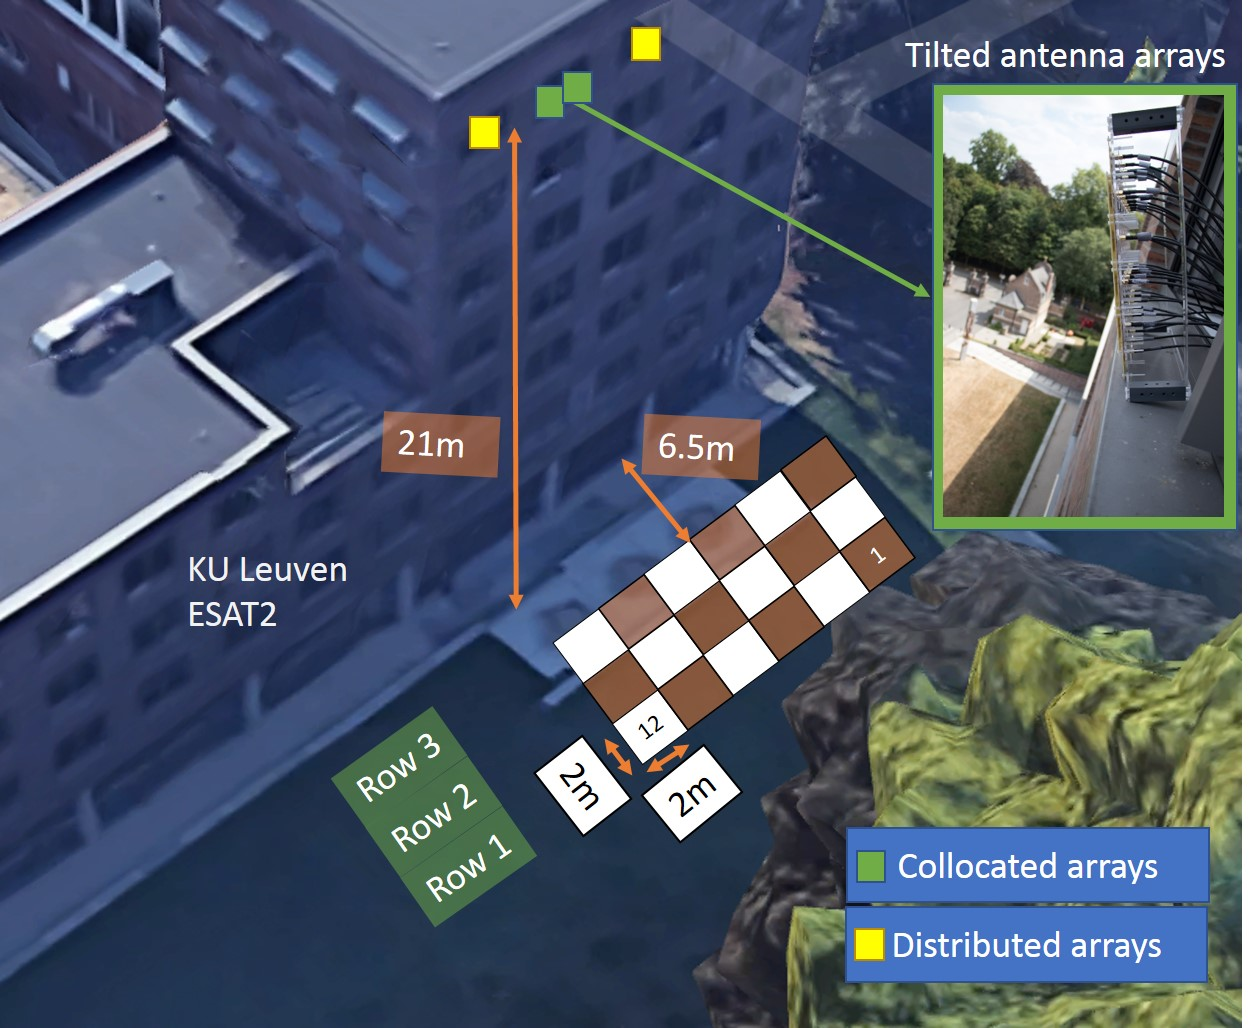
\includegraphics[width=1.0\linewidth]{figures/outdoor_scenario.jpg}
	\caption{We deployed $36$ UEs which were arranged into three rows in an outdoor LoS scenario. In each row, we put $12$ UEs, each pair of UEs are embedded in a single USRP with antenna spacing of $1.09\lambda$. Meanwhile, there were two ways of setting up the locations of the two-32 antennas patch arrays which were tilted in the front of windows for $24^\circ$ .}
	\label{fig:The measured outdoor scenario}
\end{figure}

\begin{figure}[t!]
	\centering
	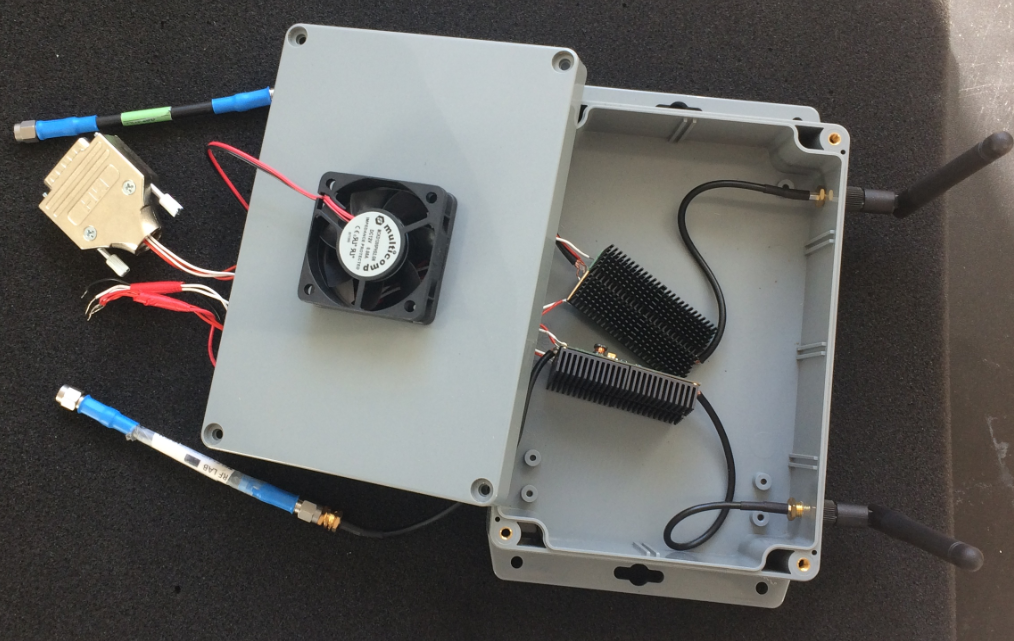
\includegraphics[width=1\linewidth]{figures/user_equipment.PNG}
	\caption{The user equipments were connected to off-the-shelf external-PAs in order to enlarge the sensitivity level for the long distance measurement. The antenna spacing is around $1.09\lambda$ for a center frequency of $2.61$GHz.}
	\label{fig:UserEquipment}
\end{figure}

\begin{figure}[t!]
	\centering
	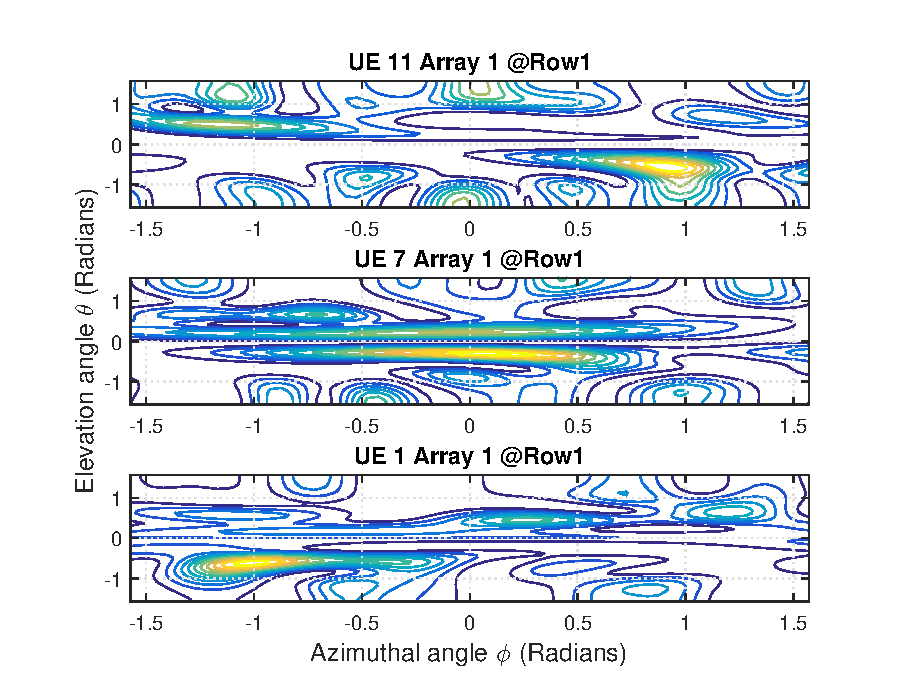
\includegraphics[width=1\linewidth]{figures/2DMUSICcollocated_row1_array1.eps}
	\caption{The 2D-MUSIC angular transformation of the measured outdoor channel. The related locations of the UEs are reflected in the angular domain.}
	\label{fig:2DMUSIC-measured-collocated-channel}
\end{figure}

\begin{figure}[t!]
	\centering
	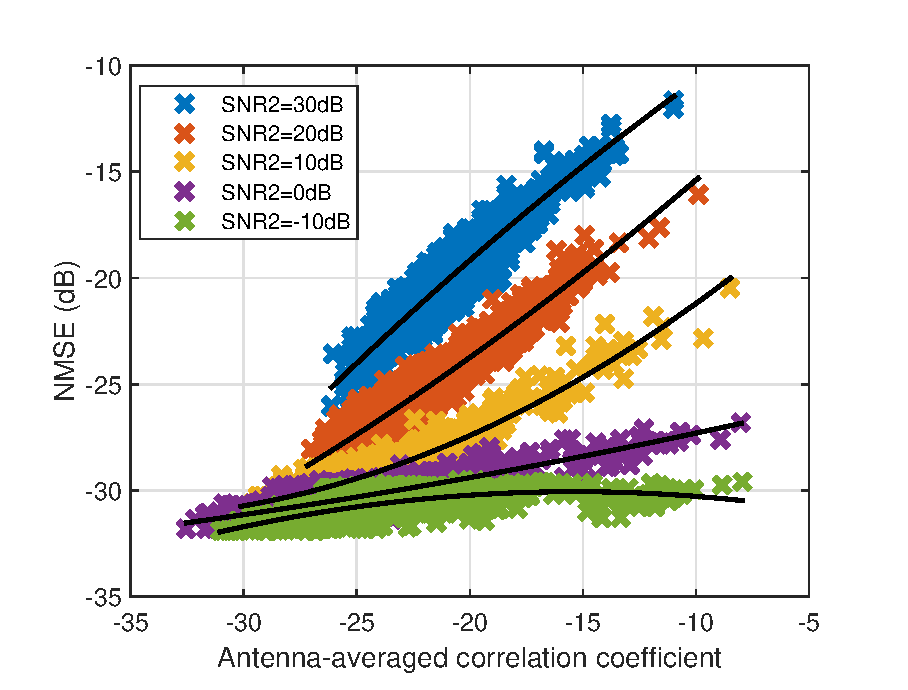
\includegraphics[width=1.0\linewidth]{figures/NMSE_correlation_allcases_collocated_wPA.eps}
	\caption{Correlation of NMSE channel estimation error to the antenna-averaged correlation coefficient. A spatially correlated channel, based on
the measured correlation channel.}
	\label{fig:channel_correlation_measured}
\end{figure}

\section{Results and discussion}
\label{results}
%\sofie{add a subsection header somewhere?}
The classification accuracies of the model for the aforementioned datasets along with the learned representations are discussed in the following subsections.

% \begin{figure}[htb]
% \begin{tikzpicture} \begin{axis}[legend pos=south east,
%  width=\columnwidth,
%  grid=both,
%  ylabel=Classification Accuracy (\%),
%   xlabel=SNR(dB),
%  grid style={line width=.1pt, draw=gray!10},
%  major grid style={line width=.2pt,draw=gray!50},
%  xmin=-20,
%  xmax=20,
%  %axis lines=middle,
%  minor tick num=5,
%  legend cell align={left},
%  %enlargelimits={abs=0.5},
%  %axis line style={latex-latex},
%  %ticklabel style={font=\tiny,fill=white},
%  %xlabel style={at={(ticklabel* cs:1)},anchor=north west},
%  %ylabel style={at={(ticklabel* cs:1)},anchor=south west}
% ]
% %[height=9cm, width=9cm, grid=major,] 
% %\addplot {-x^5 - 242}; 
% %\addlegendentry{model} 
% \addplot[mark=square, color=black] coordinates { 
% (-20, 09.807868252516011) (-18, 09.282470481380563) (-16, 09.659913169319827) (-14, 11.205341032118368) (-12, 15.332725615314494) (-10, 23.049582370712635) (-8, 37.6630534631637) (-6, 53.40909090909091) (-4, 63.99260628465804) (-2, 71.89767779390421) (0, 75.98540145985402) (2, 76.20865139949109) (4, 78.1754772393539) (6, 78.23104693140794) (8, 78.53922452660054) (10, 79.67213114754098) (12, 78.47184501176897) (14, 78.2432183059605) (16, 77.50226244343892) (18, 78.36183618361836) };
% \addlegendentry{CNN}
% \addplot[mark=diamond, color=red] coordinates { 
% ( -20 , 9.69807868253 )  ( -18 , 9.77293369664 )  ( -16 , 9.80463096961 )  ( -14 , 11.7827499098 )  ( -12 , 15.934366454 )  ( -10 , 22.69415319 )  ( -8 , 34.5948925225 )  ( -6 , 50.7881231672 )  ( -4 , 64.0480591497 )  ( -2 , 75.2539912917 )  ( 0 , 84.8175182482 )  ( 2 , 87.4045801527 )  ( 4 , 89.922907489 )  ( 6 , 90.6498194946 )  ( 8 , 90.5861136159 )  ( 10 , 90.2732240437 )  ( 12 , 90.4037660692 )  ( 14 , 90.071968998 )  ( 16 , 89.9909502262 )  ( 18 , 90.6750675068 )
% };
% \addlegendentry{LSTM:3-layer}
% \addplot[mark=o, color=blue] coordinates {
% (-20, 09.387008234217749) (-18, 08.991825613079019) (-16, 09.334298118668596) (-14, 10.285095633345363) (-12, 12.178669097538743) (-10, 35.64954682779456) (-8,  52.36083042439831) (-6,  67.46700879765396) (-4,  76.7097966728281) (-2,  82.89187227866474) (0, 88.48540145985402) (2, 90.27626317702654) (4, 92.0704845814978) (6, 91.85920577617328) (8, 92.19116321009919) (10, 91.74863387978142) (12, 91.56255658156799) (14, 91.58516331426463) (16, 91.13122171945701) (18, 91.82718271827183)
% };
% \addlegendentry{LSTM:2-layer}
% % \addplot[mark=diamond, color=green] coordinates {
% % (-20, 09.734675205855443) (-18, 09.24613987284287) (-16, 10.148335745296672) (-14, 12.630819198845183) (-12, 15.806745670009115) (-10, 24.489070552692377) (-8,  36.009553555024804) (-6,  49.12023460410557) (-4,  62.66173752310537) (-2,  76.66908563134979) (0,   85.40145985401459) (2,   88.6041439476554) (4,   90.17988252569751) (6,   90.41516245487364) (8,   90.71235347159603) (10,  90.45537340619307) (12,  90.36755386565273) (14,  89.88743310573907) (16,  90.02714932126696) (18,  90.38703870387038)
% % };
% % \addlegendentry{LSTM:2-layer: full\_snr}
% % \addplot[mark=diamond, color=purple] coordinates {
% % (-20, 09.661482159194877) (-18, 09.373297002724795) (-16, 10.256874095513749) (-14, 11.548177553229881) (-12, 15.989061075660893) (-10, 24.151412830993424) (-8,  36.67095351828036) (-6,  51.11803519061584) (-4,  62.93900184842883) (-2,  71.31712626995645) (0,   77.71897810218978) (2,   81.95201744820065) (4,   83.51688693098385) (6,   84.24187725631769) (8,   84.95942290351668) (10,  84.99089253187614) (12,  84.01231214919428) (14,  83.65011994832995) (16,  83.80090497737557) (18,  84.23042304230423)
% % };
% % \addlegendentry{LSTM:1-layer: bidir}
% \addplot[mark=triangle, color=brown] coordinates {
% (-20, 9.3870082342177488) (-18, 8.9918256130790186) (-16, 9.3342981186685964) (-14,  10.285095633345363) (-12, 12.178669097538743) (-10,19.699166364624865) (-8, 36.863319897398317) (-6, 52.61261261261261) (-4, 62.22222222222222) (-2, 72.69068959209805) (0,  79.27895120174799) (2,  82.60468548238332) (4,  83.97647923557515) (6,  84.94662565587118) (8,  85.01545735588288) (10, 84.88180318856514) (12, 84.57747764190545) (14, 84.29677651719791) (16, 84.23833819241983) (18, 84.59328425210989)
% };
% \addlegendentry{LSTM:1-layer}
% \end{axis}
% \end{tikzpicture}
% \caption{Classification accuracy comparison of hyper-parameter optimized 2-layer \textcolor{NavyBlue}{amplitude-phase} \ac{lstm} model with others on RadioML dataset.}
% \label{fig_lstm_rml_acc}
% \end{figure}

\begin{figure}[htb]
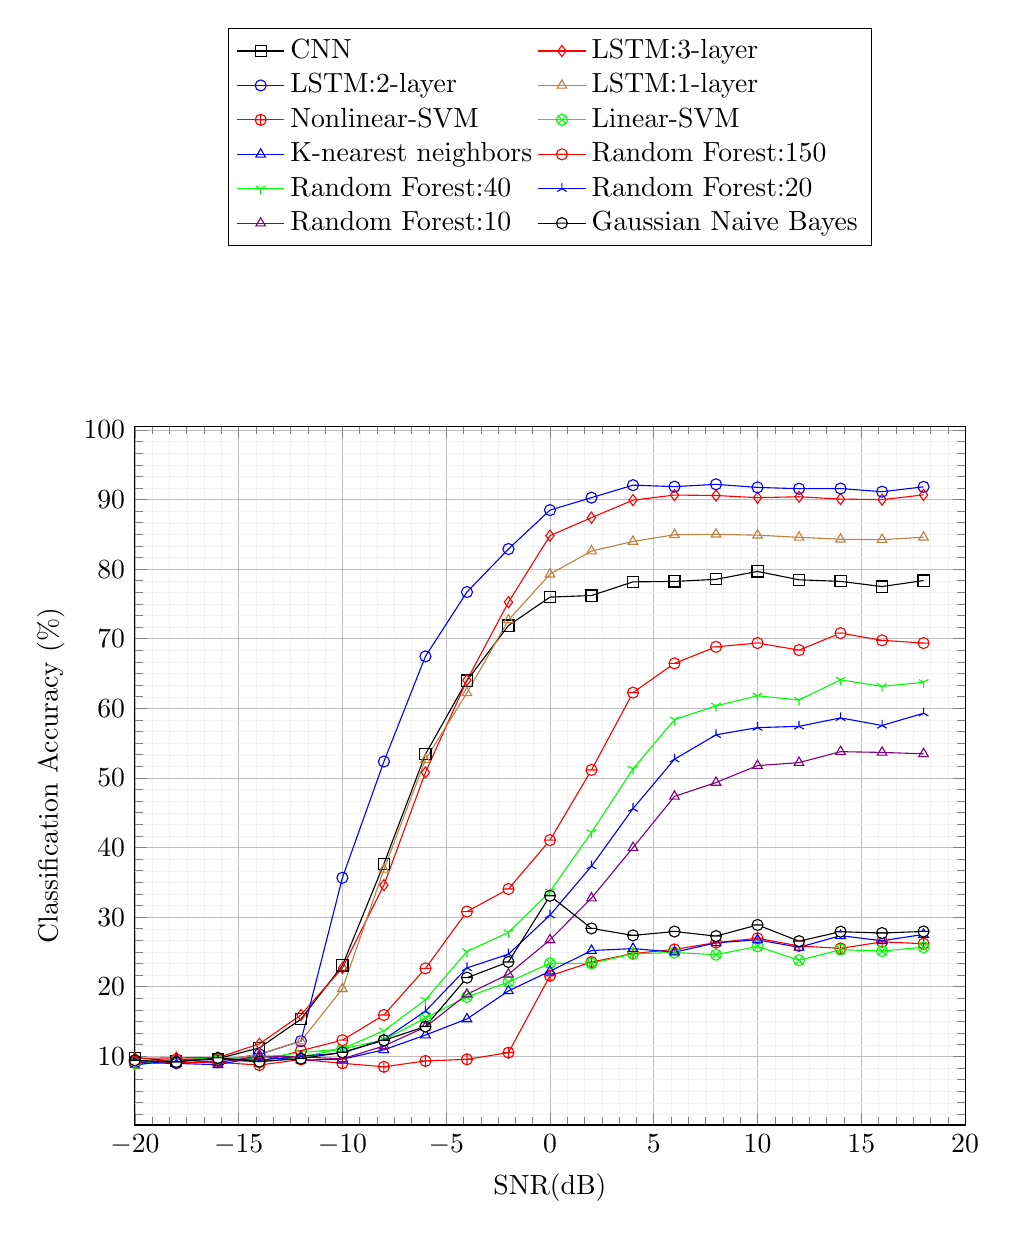
\begin{tikzpicture} \begin{axis}[legend style={at={(0.5,1.57)},anchor=north},
legend columns=2,
 width=\columnwidth,
 grid=both,
 ylabel=Classification Accuracy (\%),
  xlabel=SNR(dB),
 grid style={line width=.1pt, draw=gray!10},
 major grid style={line width=.2pt,draw=gray!50},
 xmin=-20,
 xmax=20,
 %axis lines=middle,
 minor tick num=5,
 legend cell align={left},
 %enlargelimits={abs=0.5},
 %axis line style={latex-latex},
 %ticklabel style={font=\tiny,fill=white},
 %xlabel style={at={(ticklabel* cs:1)},anchor=north west},
 %ylabel style={at={(ticklabel* cs:1)},anchor=south west}
]
%[height=9cm, width=9cm, grid=major,] 
%\addplot {-x^5 - 242}; 
%\addlegendentry{model} 
\addplot[mark=square, color=black] coordinates { 
(-20, 09.807868252516011) (-18, 09.282470481380563) (-16, 09.659913169319827) (-14, 11.205341032118368) (-12, 15.332725615314494) (-10, 23.049582370712635) (-8, 37.6630534631637) (-6, 53.40909090909091) (-4, 63.99260628465804) (-2, 71.89767779390421) (0, 75.98540145985402) (2, 76.20865139949109) (4, 78.1754772393539) (6, 78.23104693140794) (8, 78.53922452660054) (10, 79.67213114754098) (12, 78.47184501176897) (14, 78.2432183059605) (16, 77.50226244343892) (18, 78.36183618361836) };
\addlegendentry{CNN}
\addplot[mark=diamond, color=red] coordinates { 
( -20 , 9.69807868253 )  ( -18 , 9.77293369664 )  ( -16 , 9.80463096961 )  ( -14 , 11.7827499098 )  ( -12 , 15.934366454 )  ( -10 , 22.69415319 )  ( -8 , 34.5948925225 )  ( -6 , 50.7881231672 )  ( -4 , 64.0480591497 )  ( -2 , 75.2539912917 )  ( 0 , 84.8175182482 )  ( 2 , 87.4045801527 )  ( 4 , 89.922907489 )  ( 6 , 90.6498194946 )  ( 8 , 90.5861136159 )  ( 10 , 90.2732240437 )  ( 12 , 90.4037660692 )  ( 14 , 90.071968998 )  ( 16 , 89.9909502262 )  ( 18 , 90.6750675068 )
};
\addlegendentry{LSTM:3-layer}
\addplot[mark=o, color=blue] coordinates {
(-20, 09.387008234217749) (-18, 08.991825613079019) (-16, 09.334298118668596) (-14, 10.285095633345363) (-12, 12.178669097538743) (-10, 35.64954682779456) (-8,  52.36083042439831) (-6,  67.46700879765396) (-4,  76.7097966728281) (-2,  82.89187227866474) (0, 88.48540145985402) (2, 90.27626317702654) (4, 92.0704845814978) (6, 91.85920577617328) (8, 92.19116321009919) (10, 91.74863387978142) (12, 91.56255658156799) (14, 91.58516331426463) (16, 91.13122171945701) (18, 91.82718271827183)
};
\addlegendentry{LSTM:2-layer}
\addplot[mark=triangle, color=brown] coordinates {
(-20, 9.3870082342177488) (-18, 8.9918256130790186) (-16, 9.3342981186685964) (-14,  10.285095633345363) (-12, 12.178669097538743) (-10,19.699166364624865) (-8, 36.863319897398317) (-6, 52.61261261261261) (-4, 62.22222222222222) (-2, 72.69068959209805) (0,  79.27895120174799) (2,  82.60468548238332) (4,  83.97647923557515) (6,  84.94662565587118) (8,  85.01545735588288) (10, 84.88180318856514) (12, 84.57747764190545) (14, 84.29677651719791) (16, 84.23833819241983) (18, 84.59328425210989)
};
\addlegendentry{LSTM:1-layer}
\addplot[mark=oplus, color=red] coordinates {
(  -20 , 9.29551692589 )(  -18 , 9.10081743869 )(  -16 , 9.13531114327 )(  -14 , 8.73330927463 )(  -12 , 9.53509571559 )(  -10 , 8.99235827261 )(  -8 , 8.48796619511 )(  -6 , 9.32917888563 )(  -4 , 9.55637707948 )(  -2 , 10.5224963716 )(  0 , 21.5693430657 )(  2 , 23.5368956743 )(  4 , 24.7613803231 )(  6 , 25.3610108303 )(  8 , 26.3300270514 )(  10 , 26.9581056466 )(  12 , 25.855513308 )(  14 , 25.5028603063 )(  16 , 26.443438914 )(  18 , 26.1746174617 )
};
\addlegendentry{Nonlinear-SVM}
\addplot[mark=otimes, color=green] coordinates {
(  -20 , 9.02104300091 )(  -18 , 9.42779291553 )(  -16 , 9.62373371925 )(  -14 , 9.1122338506 )(  -12 , 9.89972652689 )(  -10 , 11.0716189799 )(  -8 , 12.3461326474 )(  -6 , 15.5241935484 )(  -4 , 18.5212569316 )(  -2 , 20.6640058055 )(  0 , 23.3759124088 )(  2 , 23.3369683751 )(  4 , 24.7246696035 )(  6 , 24.9097472924 )(  8 , 24.5987376014 )(  10 , 25.7923497268 )(  12 , 23.7914177078 )(  14 , 25.3183244141 )(  16 , 25.1221719457 )(  18 , 25.6705670567 )
};
\addlegendentry{Linear-SVM}
\addplot[mark=triangle, color=blue] coordinates {
(  -20 , 9.09423604758 )(  -18 , 8.97366030881 )(  -16 , 8.79160636758 )(  -14 , 9.92421508481 )(  -12 , 9.44393801276 )(  -10 , 9.57881642083 )(  -8 , 10.9314716149 )(  -6 , 13.0498533724 )(  -4 , 15.3604436229 )(  -2 , 19.3940493469 )(  0 , 22.2262773723 )(  2 , 25.1908396947 )(  4 , 25.4772393539 )(  6 , 24.963898917 )(  8 , 26.2939585212 )(  10 , 26.7395264117 )(  12 , 25.6563461887 )(  14 , 27.3297656394 )(  16 , 26.6063348416 )(  18 , 27.5067506751 )
};
\addlegendentry{K-nearest neighbors}
\addplot[mark=halfcircle, color=red] coordinates {
(  -20 , 9.11253430924 )(  -18 , 9.55495004541 )(  -16 , 9.65991316932 )(  -14 , 9.14832190545 )(  -12 , 10.8113035552 )(  -10 , 12.3156211125 )(  -8 , 15.9287157817 )(  -6 , 22.6356304985 )(  -4 , 30.7948243993 )(  -2 , 34.0348330914 )(  0 , 41.0583941606 )(  2 , 51.1450381679 )(  4 , 62.2613803231 )(  6 , 66.4620938628 )(  8 , 68.8367899008 )(  10 , 69.3806921676 )(  12 , 68.3686402318 )(  14 , 70.806421849 )(  16 , 69.7737556561 )(  18 , 69.3789378938 )
};
\addlegendentry{Random Forest:150}
% \addplot[mark=triangle, color=brown] coordinates {
% (  -20 , 9.13083257091 )(  -18 , 10.0454132607 )(  -16 , 9.28002894356 )(  -14 , 9.54529050884 )(  -12 , 10.7019143118 )(  -10 , 11.9246490137 )(  -8 , 15.3040602609 )(  -6 , 20.7661290323 )(  -4 , 28.5767097967 )(  -2 , 31.2409288824 )(  0 , 37.7189781022 )(  2 , 47.8007997092 )(  4 , 59.9853157122 )(  6 , 64.440433213 )(  8 , 67.1956717764 )(  10 , 67.3406193078 )(  12 , 66.6123483614 )(  14 , 68.5366303746 )(  16 , 68.0180995475 )(  18 , 68.0108010801 )
% };
% \addlegendentry{RF:100}
\addplot[mark=Mercedes star flipped, color=green] coordinates {
(  -20 , 8.78316559927 )(  -18 , 9.4459582198 )(  -16 , 9.76845151954 )(  -14 , 9.74377481054 )(  -12 , 10.5013673655 )(  -10 , 11.089390439 )(  -8 , 13.6689325739 )(  -6 , 18.1085043988 )(  -4 , 25.0646950092 )(  -2 , 27.793904209 )(  0 , 33.6678832117 )(  2 , 42.1664849146 )(  4 , 51.3032305433 )(  6 , 58.3754512635 )(  8 , 60.3606853021 )(  10 , 61.8032786885 )(  12 , 61.1986239363 )(  14 , 64.0893153718 )(  16 , 63.149321267 )(  18 , 63.7443744374 )
};
\addlegendentry{Random Forest:40}
\addplot[mark=Mercedes star, color=blue] coordinates {
(  -20 , 8.7648673376 )(  -18 , 9.42779291553 )(  -16 , 9.53328509407 )(  -14 , 9.45507037171 )(  -12 , 10.0091157703 )(  -10 , 10.4673893727 )(  -8 , 12.4196215322 )(  -6 , 16.4772727273 )(  -4 , 22.6987060998 )(  -2 , 24.6734397678 )(  0 , 30.2737226277 )(  2 , 37.3137041076 )(  4 , 45.5947136564 )(  6 , 52.6895306859 )(  8 , 56.1947700631 )(  10 , 57.2313296903 )(  12 , 57.4144486692 )(  14 , 58.6270529618 )(  16 , 57.5384615385 )(  18 , 59.297929793 )
};
\addlegendentry{Random Forest:20}
\addplot[mark=triangle, color=violet] coordinates {
(  -18 , 9.57311534968 )(  -16 , 9.08104196816 )(  -14 , 10.0505232768 )(  -12 , 9.91795806746 )(  -10 , 9.63213079794 )(  -8 , 11.482638251 )(  -6 , 14.2045454545 )(  -4 , 18.9094269871 )(  -2 , 21.7888243832 )(  0 , 26.7153284672 )(  2 , 32.7335514358 )(  4 , 39.9779735683 )(  6 , 47.3465703971 )(  8 , 49.3417493237 )(  10 , 51.766848816 )(  12 , 52.1998913634 )(  14 , 53.7737589961 )(  16 , 53.665158371 )(  18 , 53.4653465347 )
};
\addlegendentry{Random Forest:10}
\addplot[mark=halfcircle, color=black] coordinates {
(  -20 , 9.42360475755 )(  -18 , 9.17347865577 )(  -16 , 9.76845151954 )(  -14 , 9.23854204258 )(  -12 , 9.66271649954 )(  -10 , 10.5740181269 )(  -8 , 12.2910159838 )(  -6 , 14.2778592375 )(  -4 , 21.2939001848 )(  -2 , 23.5486211901 )(  0 , 33.0656934307 )(  2 , 28.3715012723 )(  4 , 27.3678414097 )(  6 , 27.9241877256 )(  8 , 27.2678088368 )(  10 , 28.8706739526 )(  12 , 26.5435451747 )(  14 , 27.9018269053 )(  16 , 27.7104072398 )(  18 , 27.9387938794 )
};
\addlegendentry{Gaussian Naive Bayes}
\addplot[mark=triangle, color=brown] coordinates {
};
\addlegendentry{MNB}
\addplot[mark=triangle, color=brown] coordinates {

};
\addlegendentry{SVC}
\end{axis}
\end{tikzpicture}
\caption{Classification accuracy comparison of hyper-parameter optimized 2-layer amplitude-phase \ac{lstm} model with others on RadioML dataset.}
%\label{fig_rml_comp_acc}
\label{fig_lstm_rml_acc}
\end{figure}

\begin{figure}[htb]
\centering
-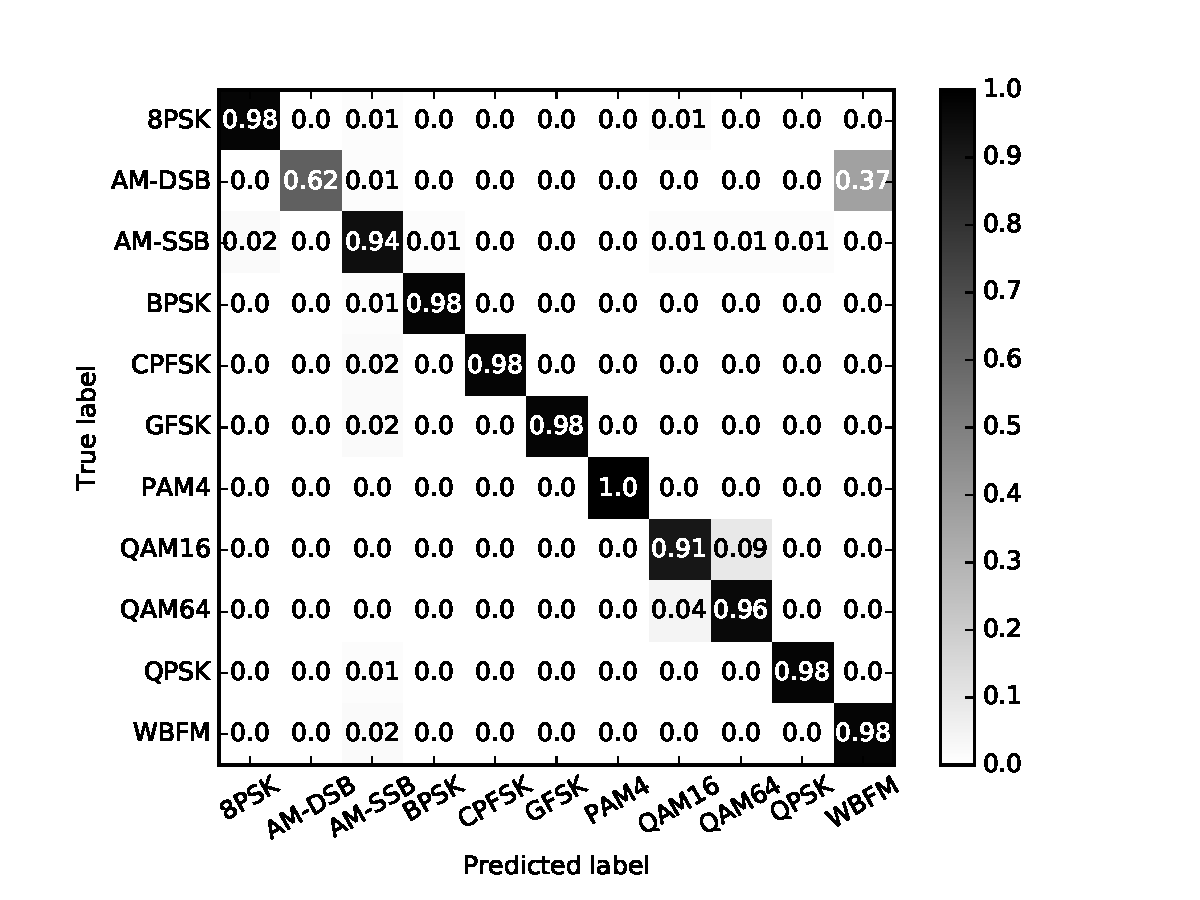
\includegraphics[width=1.1\columnwidth]{figures/confmat_18.pdf}
\caption{Confusion matrix for 2-layer amplitude-phase LSTM model on RadioML dataset at 18dB SNR} 
\label{fig_confmat_18}
\end{figure}

\begin{figure}[htb]
\centering
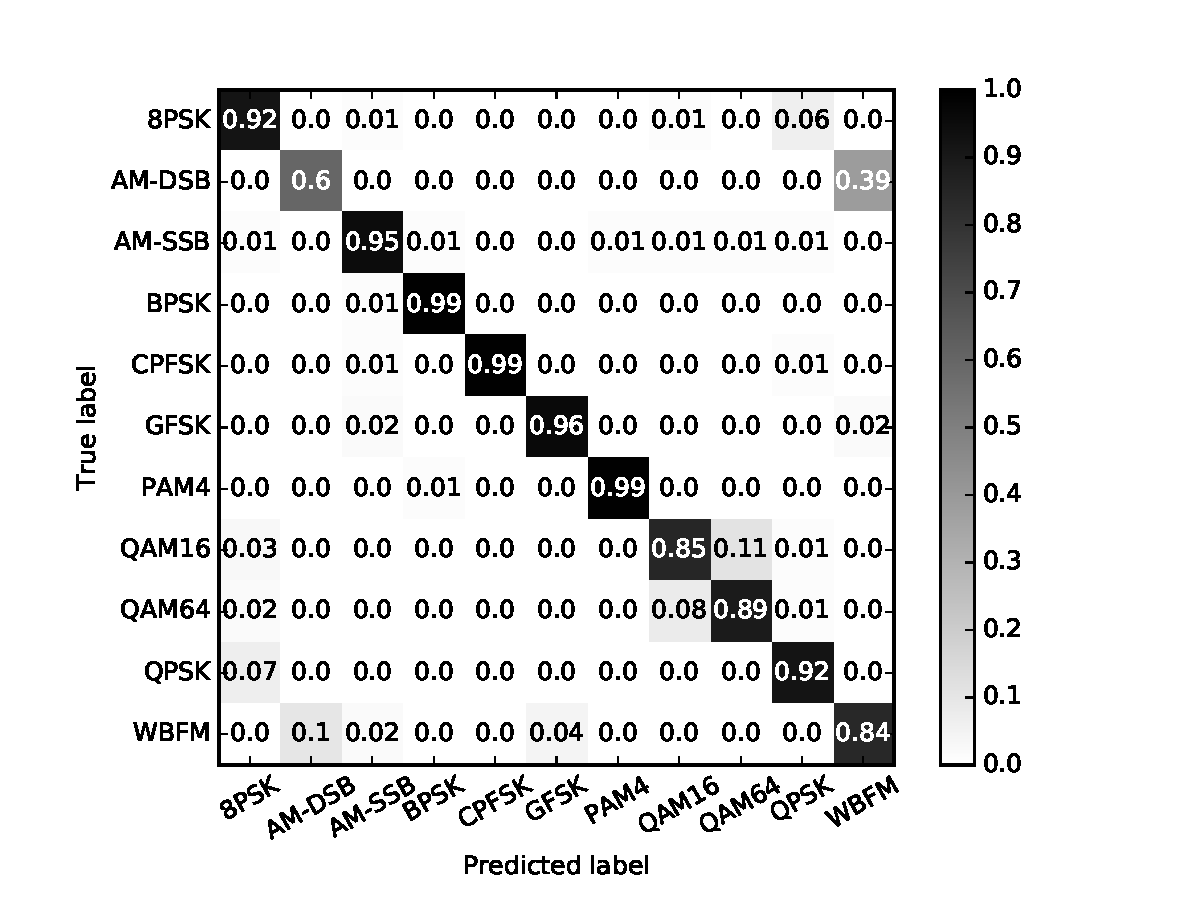
\includegraphics[width=1.1\columnwidth]{figures/confmat_0.pdf}
\caption{Confusion matrix for 2-layer amplitude-phase LSTM model on RadioML dataset at 0dB SNR} 
\label{fig_confmat_0}
\end{figure}

\begin{figure}[htb]
\centering
\squeezeup
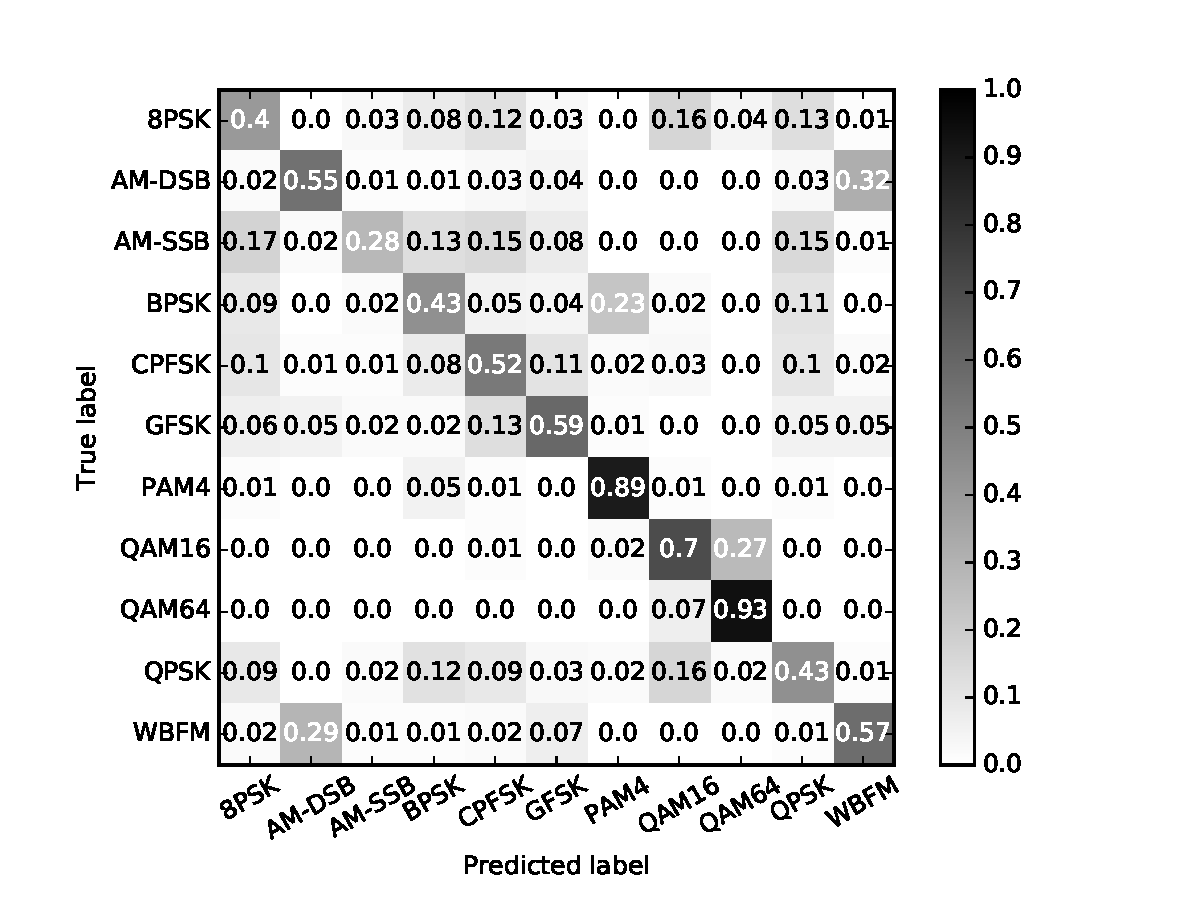
\includegraphics[width=1.1\columnwidth]{figures/confmat_-8.pdf}
\caption{Confusion matrix for 2-layer amplitude-phase LSTM model on RadioML dataset at -8dB SNR} 
\label{fig_confmat_-8}
\end{figure}

\begin{figure}[htb]
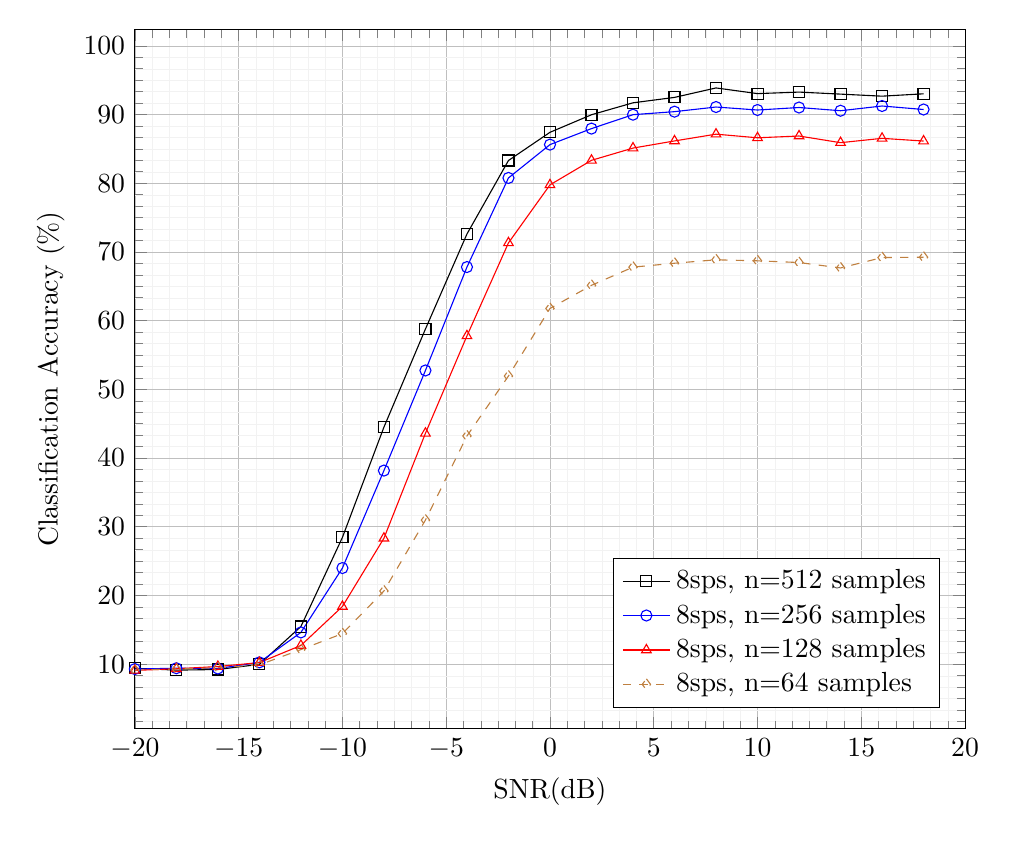
\begin{tikzpicture} \begin{axis}[legend pos=south east,
 width=\columnwidth,
 grid=both,
 ylabel=Classification Accuracy (\%),
  xlabel=SNR(dB),
 grid style={line width=.1pt, draw=gray!10},
 major grid style={line width=.2pt,draw=gray!50},
 minor tick num=5,
 xmin=-20,
 xmax=20,
 legend cell align={left},
]
\addplot[mark=square, color=black] coordinates {
(-20, 09.405306495882891) (-18, 09.137148047229791) (-16, 09.225759768451519) (-14, 09.978347167087694) (-12, 15.478577939835916) (-10, 28.45210591789586) (-8,  44.497519750137793) (-6,  58.77932551319648) (-4,  72.60628465804067) (-2,  83.30914368650217) (0,   87.40875912408759) (2,   89.96728462377317) (4,   91.70337738619677) (6,   92.49097472924188) (8,   93.86834986474302) (10,  93.04189435336976) (12,  93.26453014665942) (14,  92.96918250599742) (16,  92.66968325791856) (18,  93.01530153015302)
};
\addlegendentry{8sps, n=512 samples}
\addplot[mark=o, color=blue] coordinates {
(-20, 09.29551692589204) (-18, 09.409627611262489) (-16, 09.370477568740955) (-14, 10.267051605918441) (-12, 14.62169553327256) (-10, 23.991469699662343) (-8,  38.17747565680691) (-6,  52.74926686217009) (-4,  67.8003696857671) (-2,  80.76923076923077) (0,   85.62043795620438) (2,   87.94983642311887) (4,   89.97797356828194) (6,   90.41516245487364) (8,   91.09107303877367) (10,  90.65573770491804) (12,  91.01937352887923) (14,  90.55176231777081) (16,  91.23981900452489) (18,  90.72907290729073)
};
\addlegendentry{8sps, n=256 samples}
\addplot[mark=triangle, color=red] coordinates {
(-20, 09.09423604757548) (-18, 09.336966394187103) (-16, 09.659913169319827) (-14, 10.230963551064598) (-12, 12.725615314494074) (-10, 18.393460103074463) (-8,  28.32996509277972) (-6,  43.603372434017595) (-4,  57.7818853974122) (-2,  71.31712626995645) (0,   79.76277372262773) (2,   83.33333333333334) (4,   85.11380323054332) (6,   86.15523465703971) (8,   87.14156898106402) (10,  86.61202185792349) (12,  86.8730762266884) (14,  85.90145783354862) (16,  86.53393665158371) (18,  86.13861386138614)
};
\addlegendentry{8sps, n=128 samples}
\addplot[dashed, mark=diamond, color=brown] coordinates {
(-20, 09.149130832570906) (-18, 09.30063578564941) (-16, 09.479015918958032) (-14, 09.906171057380007) (-12, 12.123974475843209) (-10, 14.448196196907767) (-8,  20.65037663053463) (-6,  30.97507331378299) (-4,  43.21626617375231) (-2,  51.94121915820029) (0,   61.77007299270073) (2,   65.13994910941476) (4,   67.7863436123348) (6,   68.35740072202167) (8,   68.85482416591524) (10,  68.70673952641165) (12,  68.45917074053957) (14,  67.66931168112198) (16,  69.1764705882353) (18,  69.23492349234923)
};
\addlegendentry{8sps, n=64 samples}
\end{axis}
\end{tikzpicture}
\caption{Classification accuracy of amplitude-phase \ac{lstm} model on modified RadioML dataset for 8 samples/symbol. The model is trained only on input sample lengths (n) from 128 to 512. The model gives close to 70\% accuracy on 64 input samples (dashed line) which it is not trained for. }
\label{fig_lstm_modrml_acc_8sps}
\end{figure}


\begin{figure}[htb]
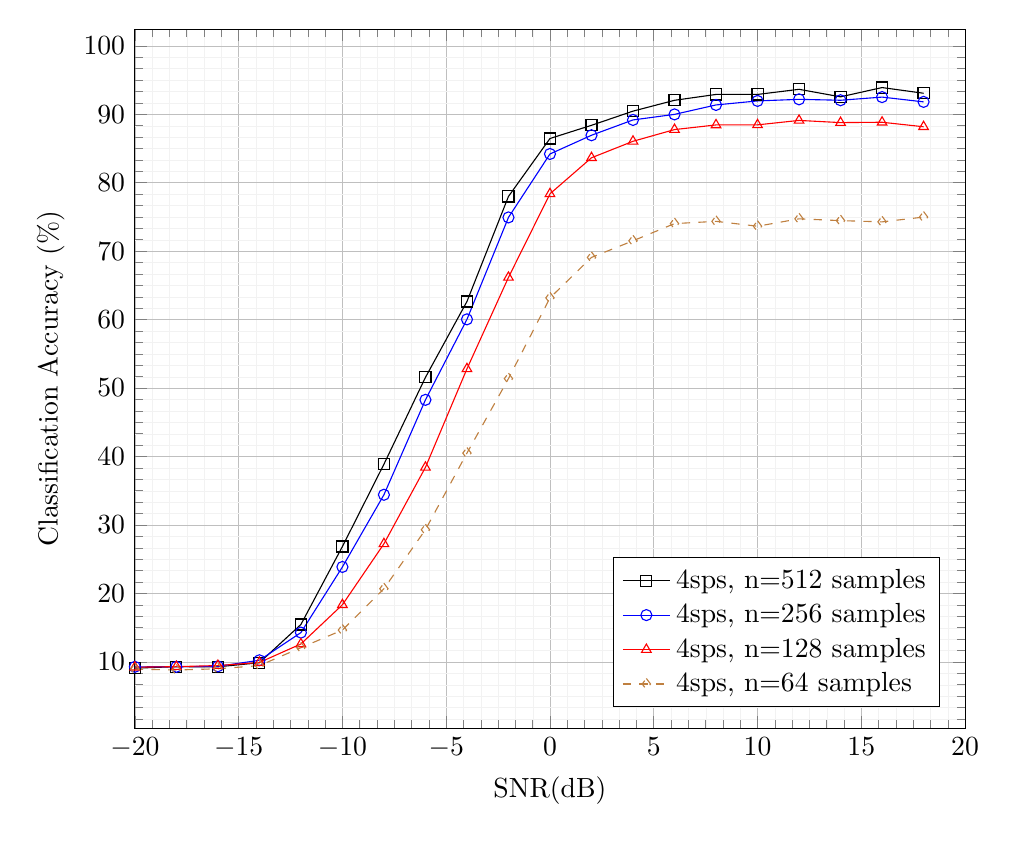
\begin{tikzpicture} \begin{axis}[legend pos=south east,
 width=\columnwidth,
 grid=both,
 ylabel=Classification Accuracy (\%),
  xlabel=SNR(dB),
 grid style={line width=.1pt, draw=gray!10},
 major grid style={line width=.2pt,draw=gray!50},
 minor tick num=5,
 xmin=-20,
 xmax=20,
 legend cell align={left},
]
\addplot[mark=square, color=black] coordinates {
(-20, 09.075937785910339) (-18, 09.30063578564941) (-16, 09.280028943560058) (-14, 09.870083002526164) (-12, 15.460346399270739) (-10, 26.852674604585036) (-8,  38.875620062465555) (-6,  51.55791788856305) (-4,  62.64325323475046) (-2,  77.99346879535559) (0,   86.45985401459854) (2,   88.38604143947656) (4,   90.45521292217328) (6,   92.03971119133574) (8,   92.89449954914337) (10,  92.89617486338798) (12,  93.64475828354155) (14,  92.54474995386602) (16,  93.90045248868778) (18,  93.06930693069307)
};
\addlegendentry{4sps, n=512 samples}
\addplot[mark=o, color=blue] coordinates {
(-20, 09.277218664226898) (-18, 09.282470481380563) (-16, 09.352387843704775) (-14, 10.230963551064598) (-12, 14.275296262534184) (-10, 23.867069486404835) (-8,  34.41117031049054) (-6,  48.277126099706746) (-4,  60.03696857670979) (-2,  74.92743105950653) (0,   84.1970802919708) (2,   86.93202471828426) (4,   89.17033773861968) (6,   89.98194945848376) (8,   91.36158701532913) (10,  91.94899817850638) (12,  92.17816404128191) (14,  92.04650304484222) (16,  92.50678733031674) (18,  91.8091809180918)
};
\addlegendentry{4sps, n=256 samples}
\addplot[mark=triangle, color=red] coordinates {
(-20, 09.222323879231473) (-18, 09.30063578564941) (-16, 09.460926193921852) (-14, 09.906171057380007) (-12, 12.61622607110301) (-10, 18.340145725964102) (-8,  27.246004041888666) (-6,  38.41642228739003) (-4,  52.80961182994455) (-2,  66.16473149492017) (0,   78.37591240875912) (2,   83.6423118865867) (4,   86.04992657856094) (6,   87.76173285198556) (8,   88.4400360685302) (10,  88.45173041894353) (12,  89.10012674271229) (14,  88.78021775235283) (16,  88.83257918552037) (18,  88.17281728172818)
};
\addlegendentry{4sps, n=128 samples}
\addplot[dashed, mark=diamond, color=brown] coordinates {
(-20, 08.947849954254346) (-18, 08.810172570390554) (-16, 08.990593342981186) (-14, 09.455070371706965) (-12, 12.069279854147676) (-10, 14.643682246312423) (-8,  20.687121072937717) (-6,  29.30718475073314) (-4,  40.499075785582256) (-2,  51.37880986937591) (0,   63.17518248175182) (2,   69.08396946564885) (4,   71.51248164464024) (6,   74.02527075812274) (8,   74.35527502254283) (10,  73.64298724954462) (12,  74.72388194821655) (14,  74.46023251522421) (16,  74.28054298642534) (18,  74.97749774977498)
};
\addlegendentry{4sps, n=64 samples}
\end{axis}
\end{tikzpicture}
\caption{Classification accuracy  of amplitude-phase \ac{lstm} model on modified RadioML dataset for 4 samples/symbol. The model is trained only on input sample lengths (n) from 128 to 512. The model gives close to 75\% accuracy on 64 input samples (dashed line) which it is not trained for.}
\label{fig_lstm_modrml_acc_4sps}
\end{figure}

\begin{figure}[htb]
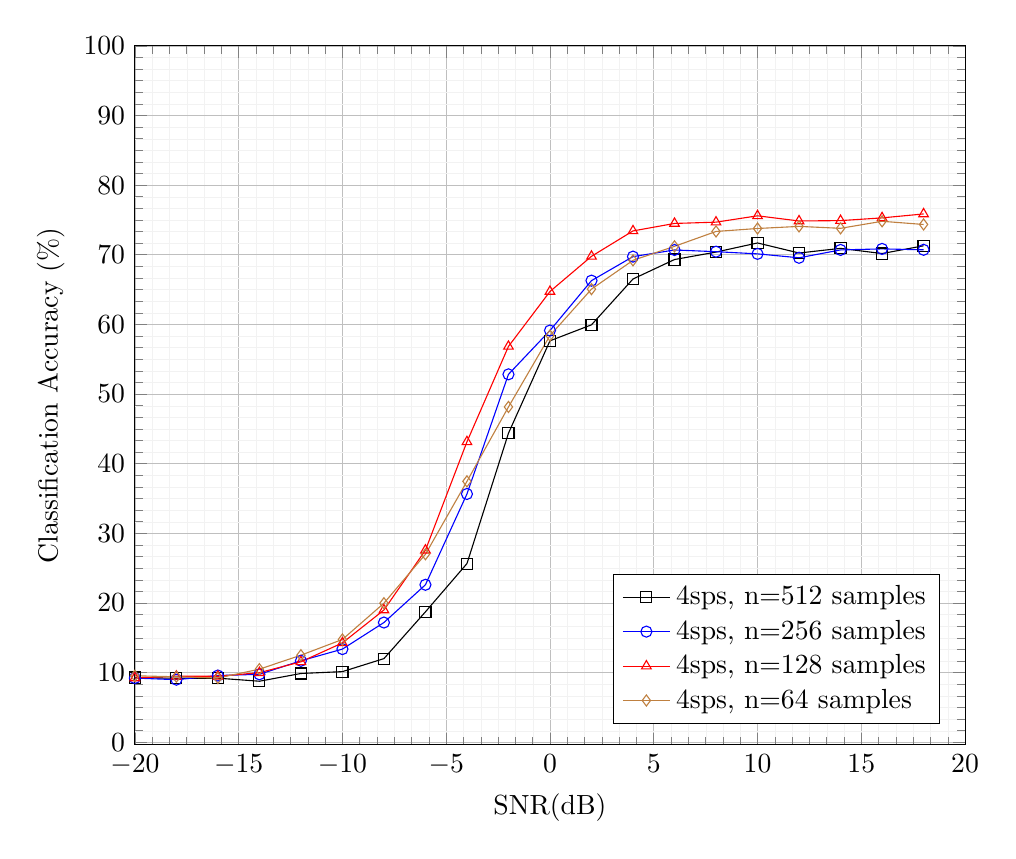
\begin{tikzpicture} \begin{axis}[legend pos=south east,
 width=\columnwidth,
 grid=both,
 ylabel=Classification Accuracy (\%),
  xlabel=SNR(dB),
 grid style={line width=.1pt, draw=gray!10},
 major grid style={line width=.2pt,draw=gray!50},
 minor tick num=5,
 xmin=-20,
 xmax=20,
 ymax=100,
 legend cell align={left},
]

\addplot[mark=square, color=black] coordinates {
(  -20 , 9.29551692589 )(  -18 , 9.19164396004 )(  -16 , 9.20767004342 )(  -14 , 8.76939732948 )(  -12 , 9.88149498633 )(  -10 , 10.14750311 )(  -8 , 12.0154326658 )(  -6 , 18.7316715543 )(  -4 , 25.6561922366 )(  -2 , 44.3759071118 )(  0 , 57.6459854015 )(  2 , 59.9418393312 )(  4 , 66.5198237885 )(  6 , 69.3140794224 )(  8 , 70.3877366997 )(  10 , 71.693989071 )(  12 , 70.2516748144 )(  14 , 70.9171433844 )(  16 , 70.1719457014 )(  18 , 71.2871287129 )
};
\addlegendentry{4sps, n=512 samples}
\addplot[mark=o, color=blue] coordinates {
(  -20 , 9.22232387923 )(  -18 , 8.99182561308 )(  -16 , 9.58755426918 )(  -14 , 9.76181883796 )(  -12 , 11.7046490428 )(  -10 , 13.3819086547 )(  -8 , 17.1963990446 )(  -6 , 22.6173020528 )(  -4 , 35.6561922366 )(  -2 , 52.8301886792 )(  0 , 59.1240875912 )(  2 , 66.2849872774 )(  4 , 69.7320117474 )(  6 , 70.6859205776 )(  8 , 70.441839495 )(  10 , 70.1275045537 )(  12 , 69.5636429477 )(  14 , 70.6957003137 )(  16 , 70.8416289593 )(  18 , 70.7110711071 )
};
\addlegendentry{4sps, n=256 samples}
\addplot[mark=triangle, color=red] coordinates {
(  -20 , 9.2406221409 )(  -18 , 9.48228882834 )(  -16 , 9.47901591896 )(  -14 , 9.99639119451 )(  -12 , 11.5587967183 )(  -10 , 14.2704816065 )(  -8 , 18.9968767224 )(  -6 , 27.5843108504 )(  -4 , 43.1423290203 )(  -2 , 56.8396226415 )(  0 , 64.7262773723 )(  2 , 69.7746274082 )(  4 , 73.4214390602 )(  6 , 74.4945848375 )(  8 , 74.6798917944 )(  10 , 75.5919854281 )(  12 , 74.8506246605 )(  14 , 74.9031186566 )(  16 , 75.2941176471 )(  18 , 75.8595859586 )

};
\addlegendentry{4sps, n=128 samples}
\addplot[mark=diamond, color=brown] coordinates {
(  -20 , 9.5516925892 )(  -18 , 9.40962761126 )(  -16 , 9.22575976845 )(  -14 , 10.5016239625 )(  -12 , 12.5068368277 )(  -10 , 14.7680824596 )(  -8 , 19.9706044461 )(  -6 , 26.9978005865 )(  -4 , 37.4676524954 )(  -2 , 48.1494920174 )(  0 , 58.3941605839 )(  2 , 65.0672482734 )(  4 , 69.1997063142 )(  6 , 71.2093862816 )(  8 , 73.3453561767 )(  10 , 73.7704918033 )(  12 , 74.072062285 )(  14 , 73.7959033032 )(  16 , 74.8054298643 )(  18 , 74.3474347435 )
};
\addlegendentry{4sps, n=64 samples}



% \addplot[mark=square, color=black] coordinates {
% (  -20 , 9.5516925892 )(  -18 , 9.40962761126 )(  -16 , 9.22575976845 )(  -14 , 10.5016239625 )(  -12 , 12.5068368277 )(  -10 , 14.7680824596 )(  -8 , 19.9706044461 )(  -6 , 26.9978005865 )(  -4 , 37.4676524954 )(  -2 , 48.1494920174 )(  0 , 58.3941605839 )(  2 , 65.0672482734 )(  4 , 69.1997063142 )(  6 , 71.2093862816 )(  8 , 73.3453561767 )(  10 , 73.7704918033 )(  12 , 74.072062285 )(  14 , 73.7959033032 )(  16 , 74.8054298643 )(  18 , 74.3474347435 )
% };
% \addlegendentry{4sps, n=64 samples}
% \addplot[mark=o, color=blue] coordinates {
% (  -20 , 9.2406221409 )(  -18 , 9.48228882834 )(  -16 , 9.47901591896 )(  -14 , 9.99639119451 )(  -12 , 11.5587967183 )(  -10 , 14.2704816065 )(  -8 , 18.9968767224 )(  -6 , 27.5843108504 )(  -4 , 43.1423290203 )(  -2 , 56.8396226415 )(  0 , 64.7262773723 )(  2 , 69.7746274082 )(  4 , 73.4214390602 )(  6 , 74.4945848375 )(  8 , 74.6798917944 )(  10 , 75.5919854281 )(  12 , 74.8506246605 )(  14 , 74.9031186566 )(  16 , 75.2941176471 )(  18 , 75.8595859586 )

% };
% \addlegendentry{4sps, n=128 samples}
% \addplot[mark=triangle, color=red] coordinates {
% (  -20 , 9.22232387923 )(  -18 , 8.99182561308 )(  -16 , 9.58755426918 )(  -14 , 9.76181883796 )(  -12 , 11.7046490428 )(  -10 , 13.3819086547 )(  -8 , 17.1963990446 )(  -6 , 22.6173020528 )(  -4 , 35.6561922366 )(  -2 , 52.8301886792 )(  0 , 59.1240875912 )(  2 , 66.2849872774 )(  4 , 69.7320117474 )(  6 , 70.6859205776 )(  8 , 70.441839495 )(  10 , 70.1275045537 )(  12 , 69.5636429477 )(  14 , 70.6957003137 )(  16 , 70.8416289593 )(  18 , 70.7110711071 )
% };
% \addlegendentry{4sps, n=256 samples}
% \addplot[mark=diamond, color=brown] coordinates {
% (  -20 , 9.29551692589 )(  -18 , 9.19164396004 )(  -16 , 9.20767004342 )(  -14 , 8.76939732948 )(  -12 , 9.88149498633 )(  -10 , 10.14750311 )(  -8 , 12.0154326658 )(  -6 , 18.7316715543 )(  -4 , 25.6561922366 )(  -2 , 44.3759071118 )(  0 , 57.6459854015 )(  2 , 59.9418393312 )(  4 , 66.5198237885 )(  6 , 69.3140794224 )(  8 , 70.3877366997 )(  10 , 71.693989071 )(  12 , 70.2516748144 )(  14 , 70.9171433844 )(  16 , 70.1719457014 )(  18 , 71.2871287129 )
% };
% \addlegendentry{4sps, n=512 samples}
\end{axis}
\end{tikzpicture}
\caption{Classification accuracy  of amplitude-phase \ac{lstm} model for non-trained data lengths on modified RadioML dataset with 4 samples/symbol.}
\label{fig_lstm_modrml_generalization}
\end{figure}

\begin{figure*}[!t]
\centering
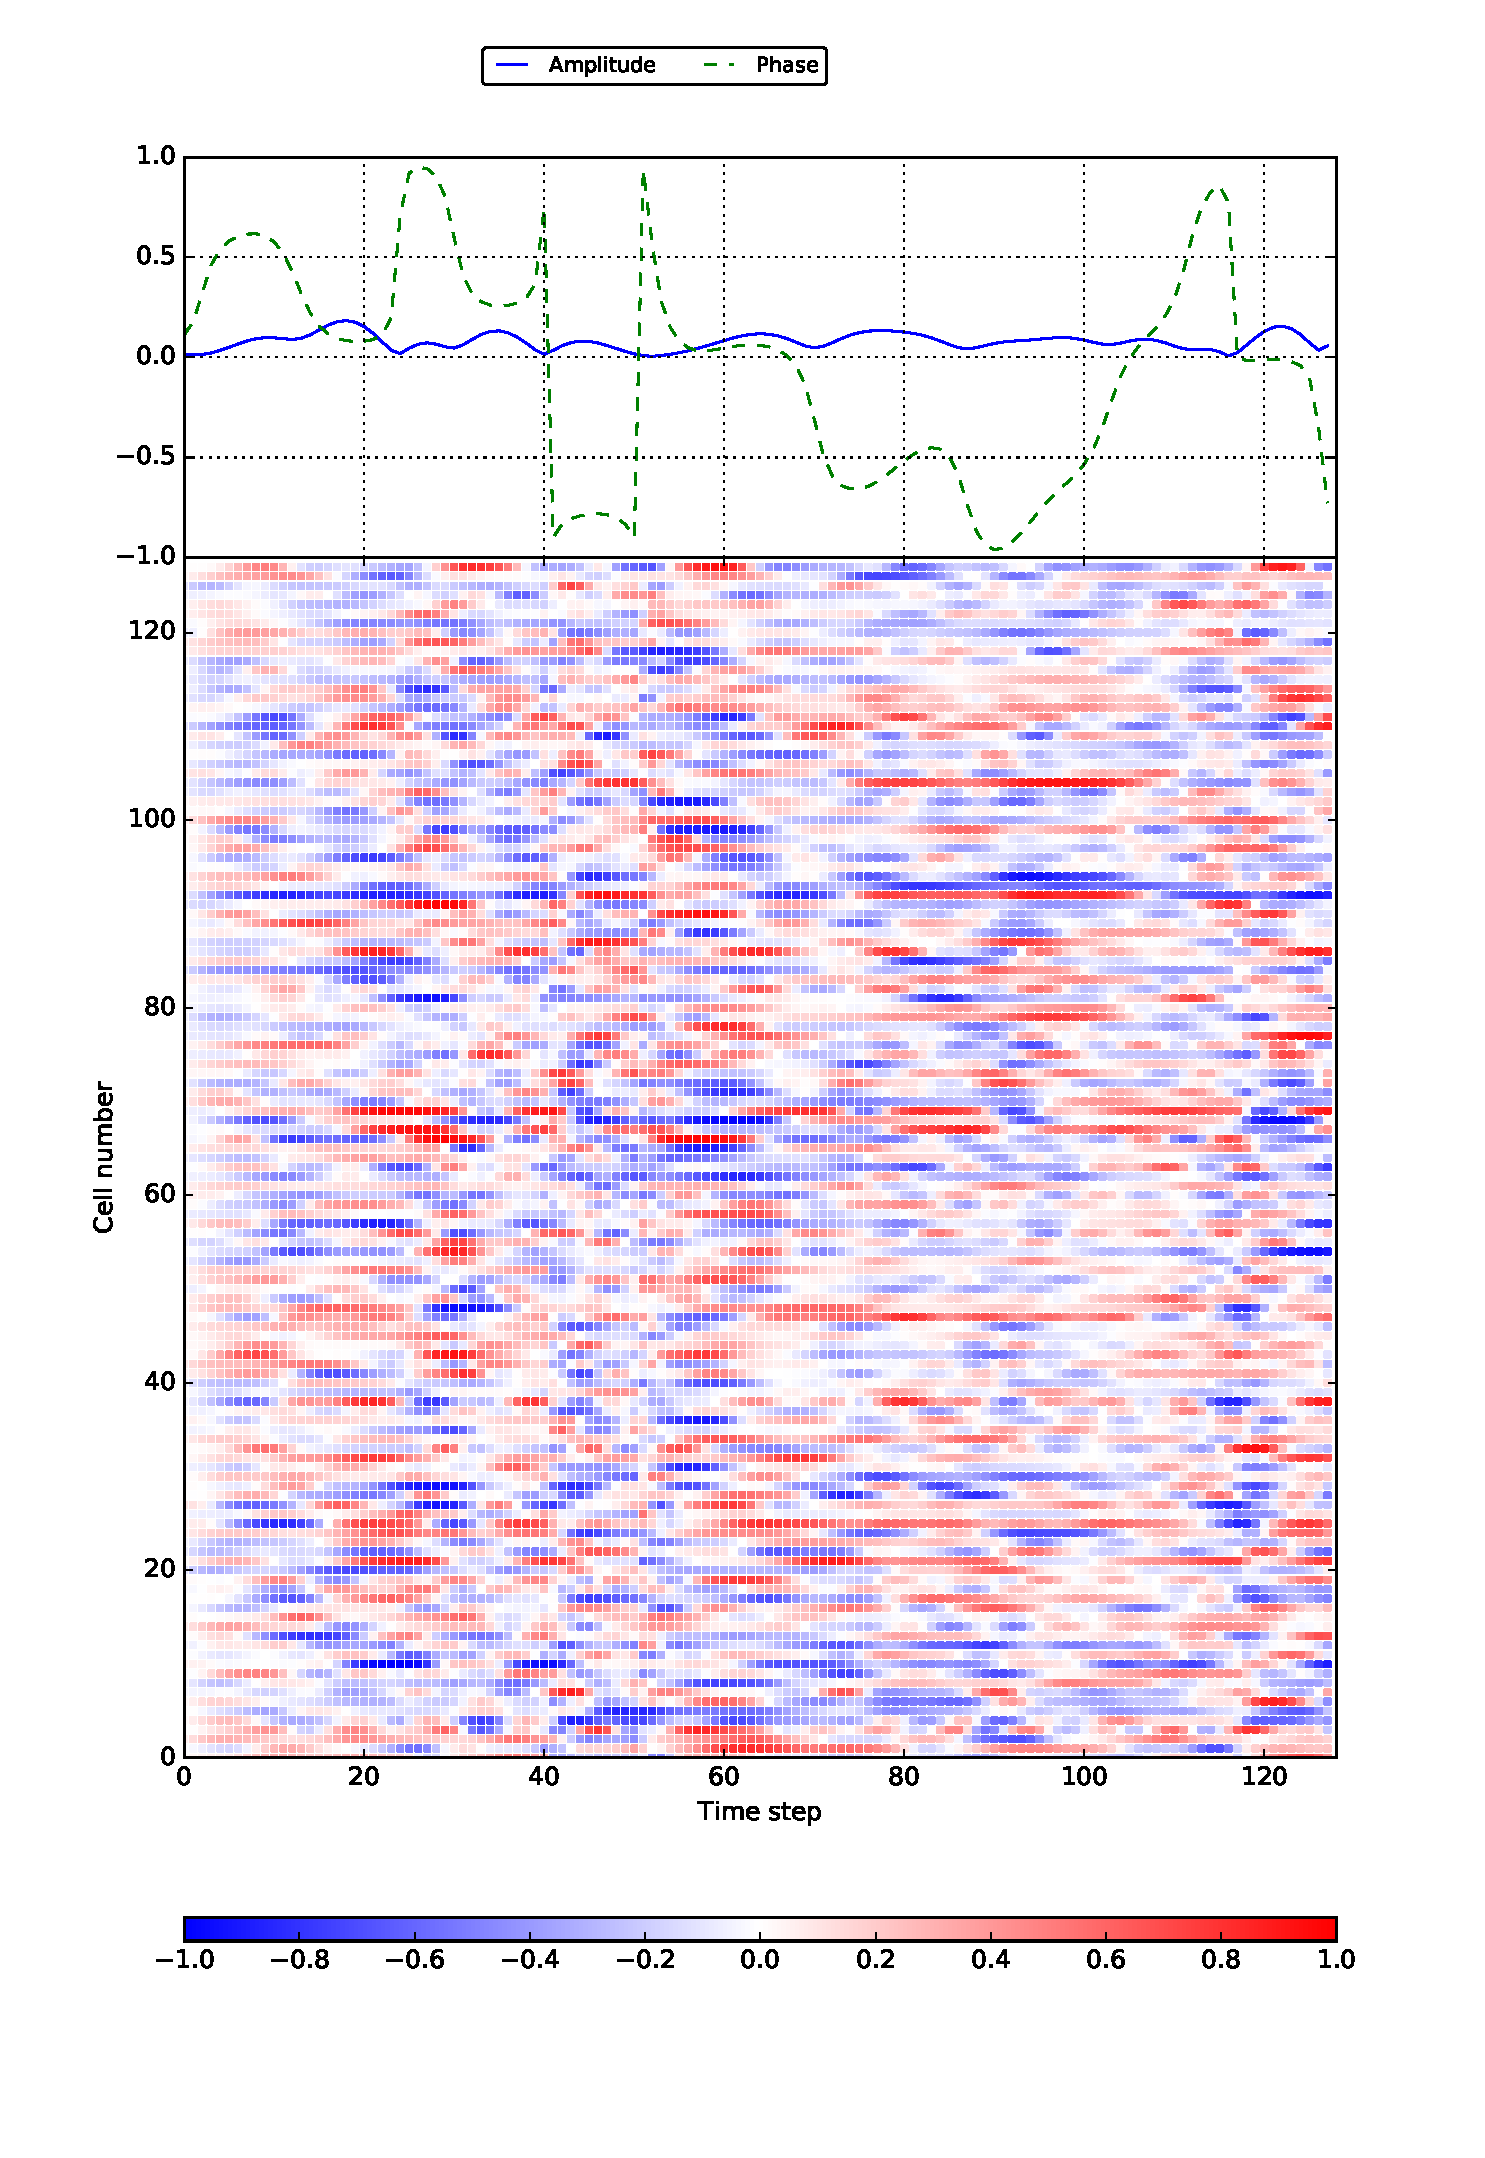
\includegraphics[width=1\columnwidth]{figures/layer_1_new1.pdf}
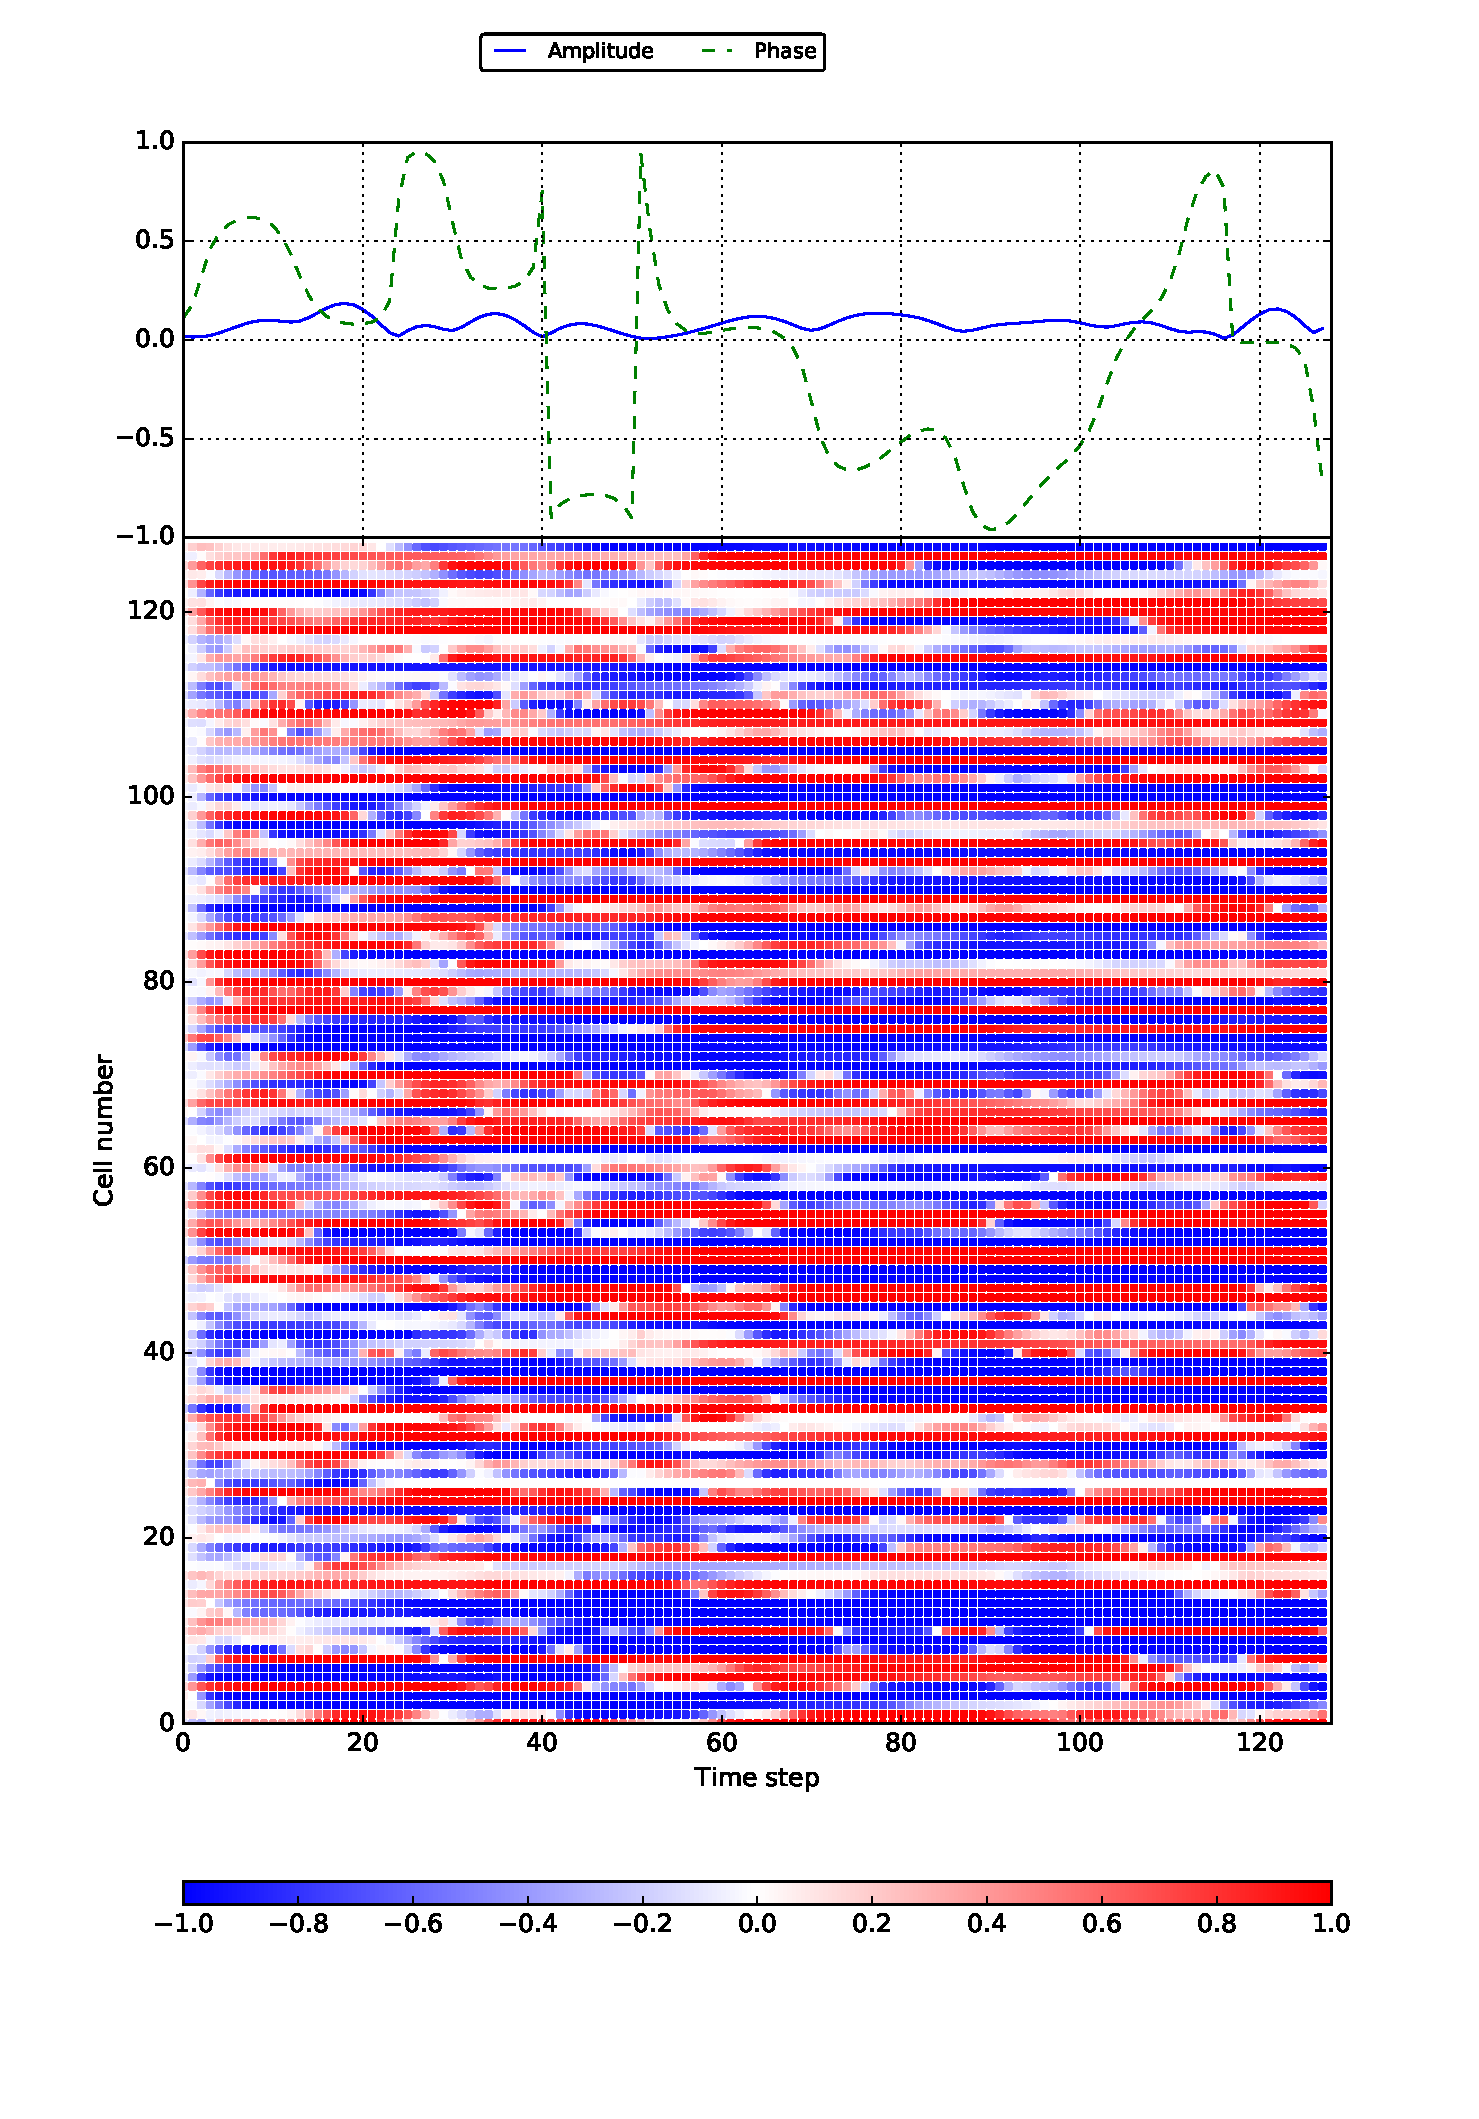
\includegraphics[width=1\columnwidth]{figures/layer_2_new1.pdf}
\caption{Layer-1 (left) and layer-2 (right) LSTM temporal activations for a QAM64 input vector. On the top the amplitude and phase of the input signal (y-axis) is plotted at each time step (x-axis). Below the amplitude and phase of the signal, temporal activations for all cells in the \ac{lstm} model for each time step are shown. Blue denotes \textit{tanh(c)} activations of value -1 and red denotes a value of +1.} 
\label{fig_activations}
\end{figure*}

\begin{figure*}[!t]
\centering
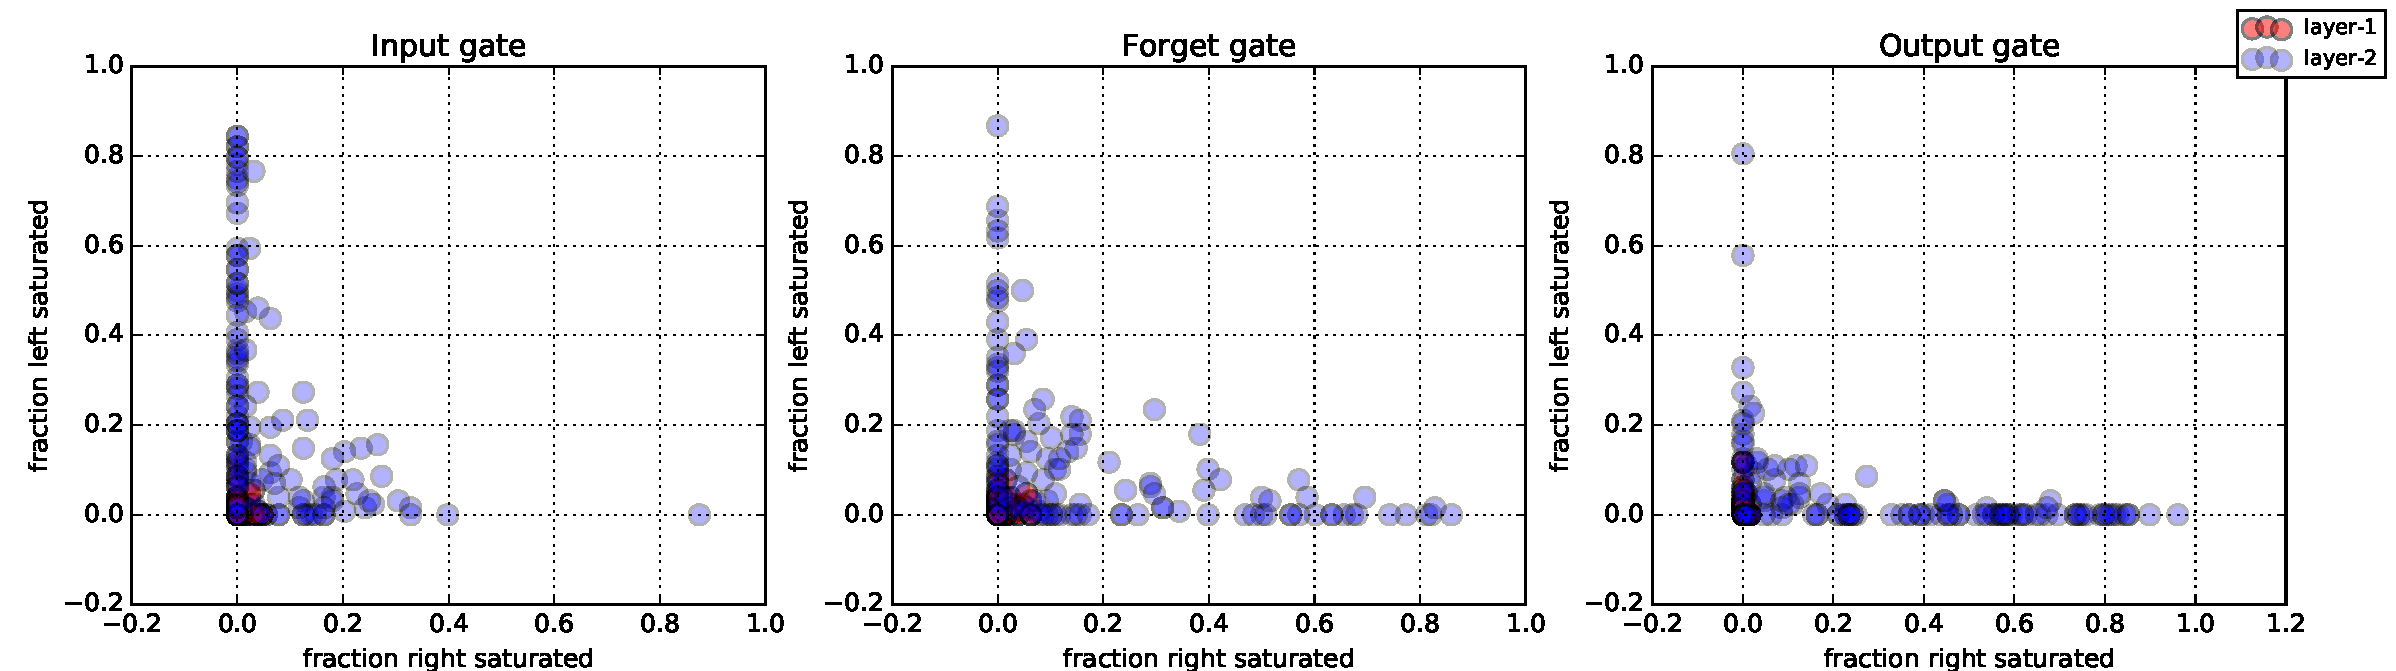
\includegraphics[width=2\columnwidth]{figures/gate_sat.pdf}
\caption{Gate saturation plots for LSTM for the same a QAM64 input vector. A circle represents a gate in a particular LSTM cell.} 
\label{fig_gatesat}
\end{figure*}



\subsection{Classification accuracy on RadioML dataset}
%\vincent{At the end of Section V.A, you mention how your normalize the amplitude and phase for the input to the model. This information should already be provided in Section IV as it seems an important design decision.}
The two layer amplitude-phase \ac{lstm} model, shown in Figure~\ref{fig_iq_lstm_model}, is trained on SNR ranges from -10dB to 20dB. Training vectors with SNR ranges below -10dB were not used as the model was converging slowly when those vectors were used. Alternate models with varying \ac{lstm} layer depths are also trained to understand the performance improvements provided by the different layer depths. The classification accuracy of all the four models are presented in Figure~\ref{fig_lstm_rml_acc}. The two layer \ac{lstm} model gave an average accuracy of 90\% in \ac{snr} ranges from 0dB to 20dB. It can be noticed that the single layer \ac{lstm} also reaches a high accuracy at high \ac{snr}s, 6\% less than the two layer model. It was also noticed that the classification accuracy saturates for layer depths of two. Hence, layer depth of two is selected for the final model and its parameters are fine tuned (dropout = 0.8 and learning rate = 0.001) to achieve the best test performance as shown in Figure~\ref{fig_lstm_rml_acc}. Rigorous fine tuning was not performed on layer depths other than two accounting for a slightly lower accuracy levels, for instance the accuracy level for layer depth 3 is slightly lower than layer depth two.  The performance of the baseline \ac{cnn} model was shown to be much better on the low \ac{snr} regions in \cite{baseline}. We were not able to reproduce the reported results on the low \ac{snr} regions after various attempts, which may be because of the difference in hyper-parameter tuning. Though, the high \ac{snr} results of the baseline model matches with that of the reported ones in the paper. Detailed discussions on the effect of layer depth and number of \ac{lstm} cells are presented in Section~\ref{sec_hyperparams}.

Classification performance of other standard machine learning models such as \ac{svm}, random forest, k-nearest neighbors and Gaussian Naive Bayes are also summarized in Figure~\ref{fig_lstm_rml_acc}. All models are fed with the same amplitude-phase training and test data for this comparison. Random forest with 150 decision trees is able to provide close to 70\% of accuracy at very high \ac{snr} conditions while others could reach only around 26\%. It could be clearly noticed that the deep learning models perform superior to the other standard techniques when fed with the raw sensed data. The deep learning models can classify signals very efficiently with a very low number of symbols, usually with hundreds of samples (tens of modulated symbols) when compared to the classical cyclostationary based expert feature models which requires samples in thousands range (hundreds of modulated symbols) for averaging. Similarly extracting expert cyclostationary features using tens of symbols is very suboptimal, which substantiate the use of deep learning models.

To understand the results better confusion matrices for the two layer \ac{lstm} model for various \ac{snr}s are also included. It can be seen in Figure~\ref{fig_confmat_18} that at a high \ac{snr} of 18dB the diagonal is much more sharp even though there are difficulties in separating AM-DSB and WBFM signals. This is mainly due to the silence periods of audio as the modulated signals are generated from real audio streams.  Similarly in Figure~\ref{fig_confmat_0}, at 0dB \ac{snr} it is noticed that there is some level of confusion regarding QAM16 and QAM64 as the former is a subset of the the latter. The confusion increases further at low \ac{snr}s as shown in Figure~\ref{fig_confmat_-8}. From these basic analysis it is clear that deep complex structures as mentioned in \cite{baseline} are not required to achieved good \ac{soa} classification accuracy at high \ac{snr}s. However, use of convolutional layers might turn useful at low \ac{snr}s as reported in \cite{baseline}. In our experiments we also noticed that simply providing \ac{iq} samples to the \ac{lstm} model yielded poor results while normalized amplitude and phase interpretation provided good results. The models even failed to reduce the training loss when fed with time domain \ac{iq} samples, giving a constant accuracy of 9\% on the radioML dataset, as the \ac{lstm}s were not able to extract any meaningful representations. Similarly feeding amplitude-phase information to the \ac{cnn} model did not provide any accuracy improvements over the \ac{iq}-\ac{cnn} model. The classification accuracy improvement is achieved from the combined benefits of using amplitude-phase information along with 2-layer \ac{lstm} model.

\subsection{Classification accuracy on modified RadioML dataset}
The same two layer \ac{lstm} model is trained on SNRs ranging from -20dB to 20dB and input sample lengths from 128 to 512 samples. The accuracy of the model is tested on the full range of SNRs and also on input sample length that is smaller than the training set (e.g, 64). It is evident from the results in Figures~\ref{fig_lstm_modrml_acc_8sps} and \ref{fig_lstm_modrml_acc_4sps} that the classification accuracy improves as the model sees more modulated symbols. Even though the model is trained on varying data lengths from 128 to 512 samples, it gives an average accuracy of 75\% with 64 samples and 4 samples per symbol scenario for which it was not trained, which confirms the model's generalization capabilities. To further analyze the generalization capabilities of the model on unseen sample lengths, four balanced folds of data each containing sequences with sample lengths of 64, 128, 256 and 512 are created. The model is then trained only on three folds, and the left-out fold is used to test generalization to the unseen length. This process is repeated for all four sample lengths and the results are presented in Figure~\ref{fig_lstm_modrml_generalization}. The model consistently gives an average accuracy above 70\% for high SNR conditions. 

\begin{figure}[htb]
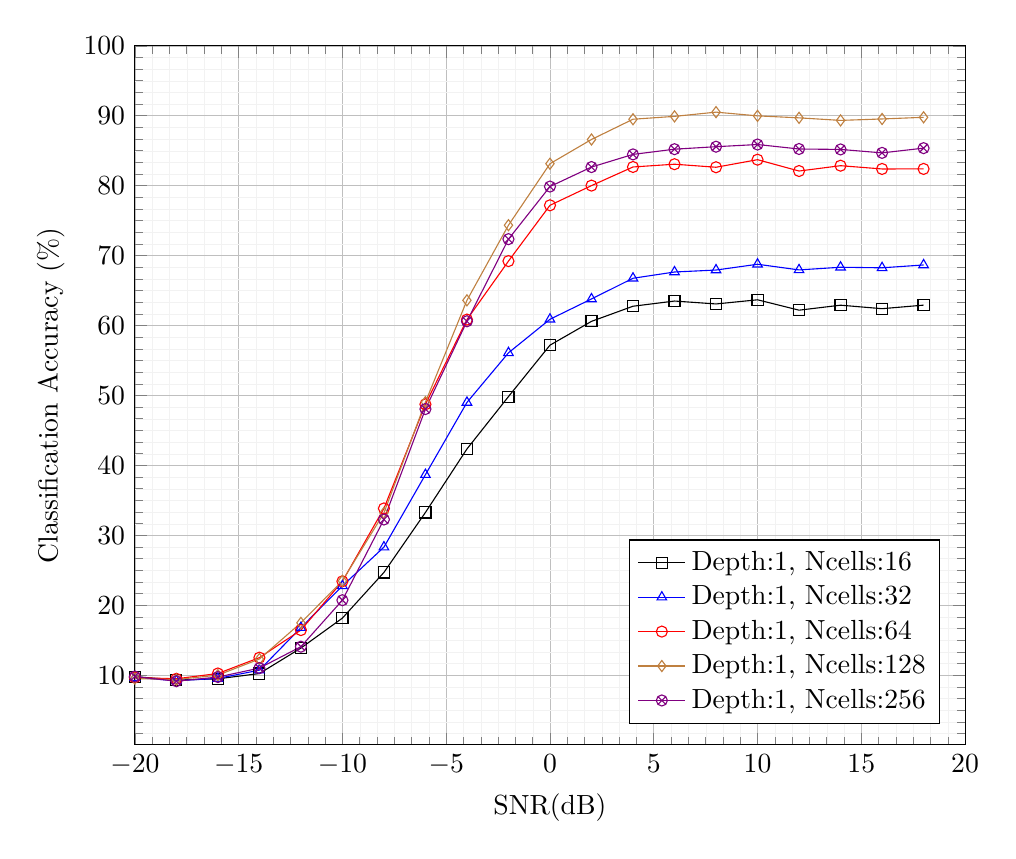
\begin{tikzpicture} \begin{axis}[legend pos=south east,
 width=\columnwidth,
 grid=both,
 ylabel=Classification Accuracy (\%),
  xlabel=SNR(dB),
 grid style={line width=.1pt, draw=gray!10},
 major grid style={line width=.2pt,draw=gray!50},
 minor tick num=5,
 xmin=-20,
 xmax=20,
 ymax=100,
 legend cell align={left},
]

\addplot[mark=square, color=black] coordinates { 
( -20 , 9.78956999085 )  ( -18 , 9.30063578565 )  ( -16 , 9.47901591896 )  ( -14 , 10.2309635511 )  ( -12 , 13.8742023701 )  ( -10 , 18.1624311356 )  ( -8 , 24.6922652949 )  ( -6 , 33.2661290323 )  ( -4 , 42.3475046211 )  ( -2 , 49.8367198839 )  ( 0 , 57.1897810219 )  ( 2 , 60.5961468557 )  ( 4 , 62.7569750367 )  ( 6 , 63.5018050542 )  ( 8 , 63.0838593327 )  ( 10 , 63.679417122 )  ( 12 , 62.1944595329 )  ( 14 , 62.9082856616 )  ( 16 , 62.407239819 )  ( 18 , 62.9162916292 )
};
\addlegendentry{Depth:1, Ncells:16}
\addplot[mark=triangle, color=blue] coordinates { 
( -20 , 9.66148215919 )  ( -18 , 9.20980926431 )  ( -16 , 9.53328509407 )  ( -14 , 10.7181522916 )  ( -12 , 16.7912488605 )  ( -10 , 22.7652390261 )  ( -8 , 28.3115928716 )  ( -6 , 38.6730205279 )  ( -4 , 49.0018484288 )  ( -2 , 56.0957910015 )  ( 0 , 60.8941605839 )  ( 2 , 63.7949836423 )  ( 4 , 66.7584434655 )  ( 6 , 67.6534296029 )  ( 8 , 67.9350766456 )  ( 10 , 68.7613843352 )  ( 12 , 67.9521998914 )  ( 14 , 68.3336408932 )  ( 16 , 68.2533936652 )  ( 18 , 68.6588658866 ) 
};
\addlegendentry{Depth:1, Ncells:32}
\addplot[mark=o, color=red] coordinates { 
( -20 , 9.66148215919 )  ( -18 , 9.48228882834 )  ( -16 , 10.2387843705 )  ( -14 , 12.5045110069 )  ( -12 , 16.4448495898 )  ( -10 , 23.4227830105 )  ( -8 , 33.8416314532 )  ( -6 , 48.7353372434 )  ( -4 , 60.8502772643 )  ( -2 , 69.2126269956 )  ( 0 , 77.1897810219 )  ( 2 , 80.0072700836 )  ( 4 , 82.6725403818 )  ( 6 , 83.0685920578 )  ( 8 , 82.6330027051 )  ( 10 , 83.7158469945 )  ( 12 , 82.093065363 )  ( 14 , 82.8566156117 )  ( 16 , 82.3891402715 )  ( 18 , 82.3942394239 ) 
};
\addlegendentry{Depth:1, Ncells:64}
\addplot[mark=diamond, color=brown] coordinates { 
( -20 , 9.51509606587 )  ( -18 , 9.37329700272 )  ( -16 , 10.003617945 )  ( -14 , 12.3060267052 )  ( -12 , 17.484047402 )  ( -10 , 23.4938688466 )  ( -8 , 33.1986037112 )  ( -6 , 49.0469208211 )  ( -4 , 63.6044362292 )  ( -2 , 74.3468795356 )  ( 0 , 83.1386861314 )  ( 2 , 86.604870956 )  ( 4 , 89.5007342144 )  ( 6 , 89.9097472924 )  ( 8 , 90.5139765555 )  ( 10 , 89.9817850638 )  ( 12 , 89.6976281007 )  ( 14 , 89.333825429 )  ( 16 , 89.5384615385 )  ( 18 , 89.7749774977 ) 
};
\addlegendentry{Depth:1, Ncells:128}
\addplot[mark=otimes, color=violet] coordinates { 
( -20 , 9.80786825252 )  ( -18 , 9.13714804723 )  ( -16 , 9.73227206946 )  ( -14 , 11.0068567304 )  ( -12 , 14.0747493163 )  ( -10 , 20.7215212369 )  ( -8 , 32.2616204299 )  ( -6 , 48.0571847507 )  ( -4 , 60.6099815157 )  ( -2 , 72.351233672 )  ( 0 , 79.8722627737 )  ( 2 , 82.6608505998 )  ( 4 , 84.4713656388 )  ( 6 , 85.2166064982 )  ( 8 , 85.572587917 )  ( 10 , 85.883424408 )  ( 12 , 85.2435270686 )  ( 14 , 85.1817678538 )  ( 16 , 84.6877828054 )  ( 18 , 85.3645364536 ) 
};
\addlegendentry{Depth:1, Ncells:256}
\end{axis}
\end{tikzpicture}
\caption{Classification accuracy of single layer amplitude-phase \ac{lstm} model for different cell size on RadioML dataset.}
\label{fig_depth_1}
\end{figure}

\subsection{Learned representations}

The inherent non-linearity and deep structures makes understanding the representations learned by \ac{lstm}s difficult. In order to obtain some good insights we use visualization techniques similar to the ones presented in \cite{vis_karpathy}. These visualizations can help to understand how \ac{lstm} cells behave for an input signal, for instance which cells gets activated at each time step and how long each gate remains open. Figures~\ref{fig_activations} and \ref{fig_gatesat} presents the gate activation and saturation of the trained two layer \ac{lstm} model for a QAM64 input signal with 18dB \ac{snr}. As explained in Section~\ref{lstm_primer} the gates of \ac{lstm} cells have sigmoid activation functions, giving an output value between 0 and 1. A gate is said to be left saturated if its activation is less than 0.1 and right saturated if the activation is greater than 0.9. The fraction of time for which the gate is in left or right saturated mode in the entire 128 samples time is plotted in Figure~\ref{fig_gatesat}. On the first layer, it can be noticed that all the three gates are confined close to the origin showing that they are not highly left or right saturated. The absence of right saturation in the first layer forget gates, confirms that the cells do not store information for long term. There are no cells in the first layer that function in purely feed-forward fashion, since their forget gates would show up as consistently left-saturated. The output gate plots in the first layer also show that there are no cells that are revealed or blocked to the hidden state. This is also visible in the activation plots of the first layer in Figure~\ref{fig_activations}. The activations are short when compared to the second layer and it can be noticed in Figure~\ref{fig_activations} that many cell activations follow the input amplitude and phase changes in the input waveform. The second layer stores much long term dependencies from the fine grained representations generated from the first layer. 


% \begin{figure*}
% \begin{minipage}[c][20cm][t]{.3\textwidth}
%   \vspace*{\fill}
%   \centering
%   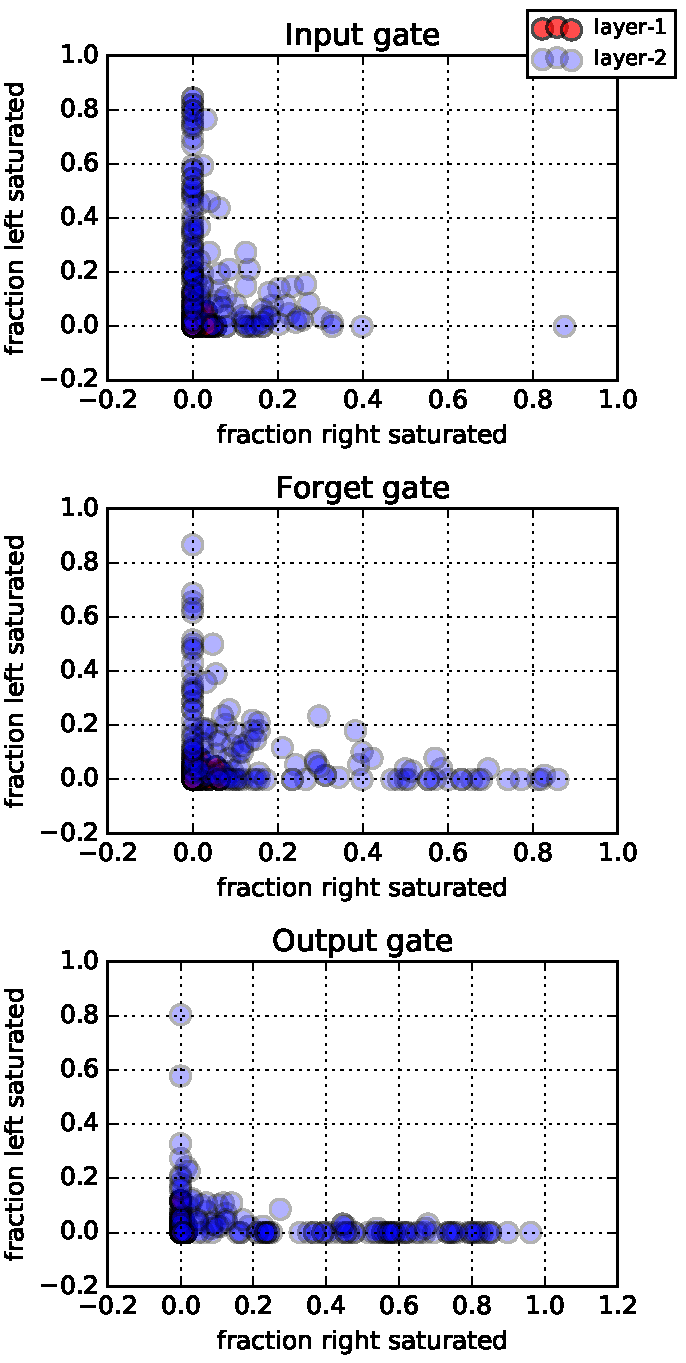
\includegraphics[width=\columnwidth,height=10cm]{figures/gate_sat_vert.pdf}
%   \caption{test figure one}
%   \label{fig:test1}
% \end{minipage}%
% \begin{minipage}[c][20cm][t]{.7\textwidth}
%   \vspace*{\fill}
%   \centering
%   \includegraphics[width=\columnwidth,height=10cm]{figures/layer_1.pdf}
%   \caption{test figure two}
%   \label{fig:test2}\par\vfill
%   \includegraphics[width=\columnwidth,height=10cm]{figures/layer_2.pdf}
%   \caption{test figure three}
%   \label{fig:test3}
% \end{minipage}
% \end{figure*}



% \begin{figure}[!t]
% \centering
% \squeezeup
% 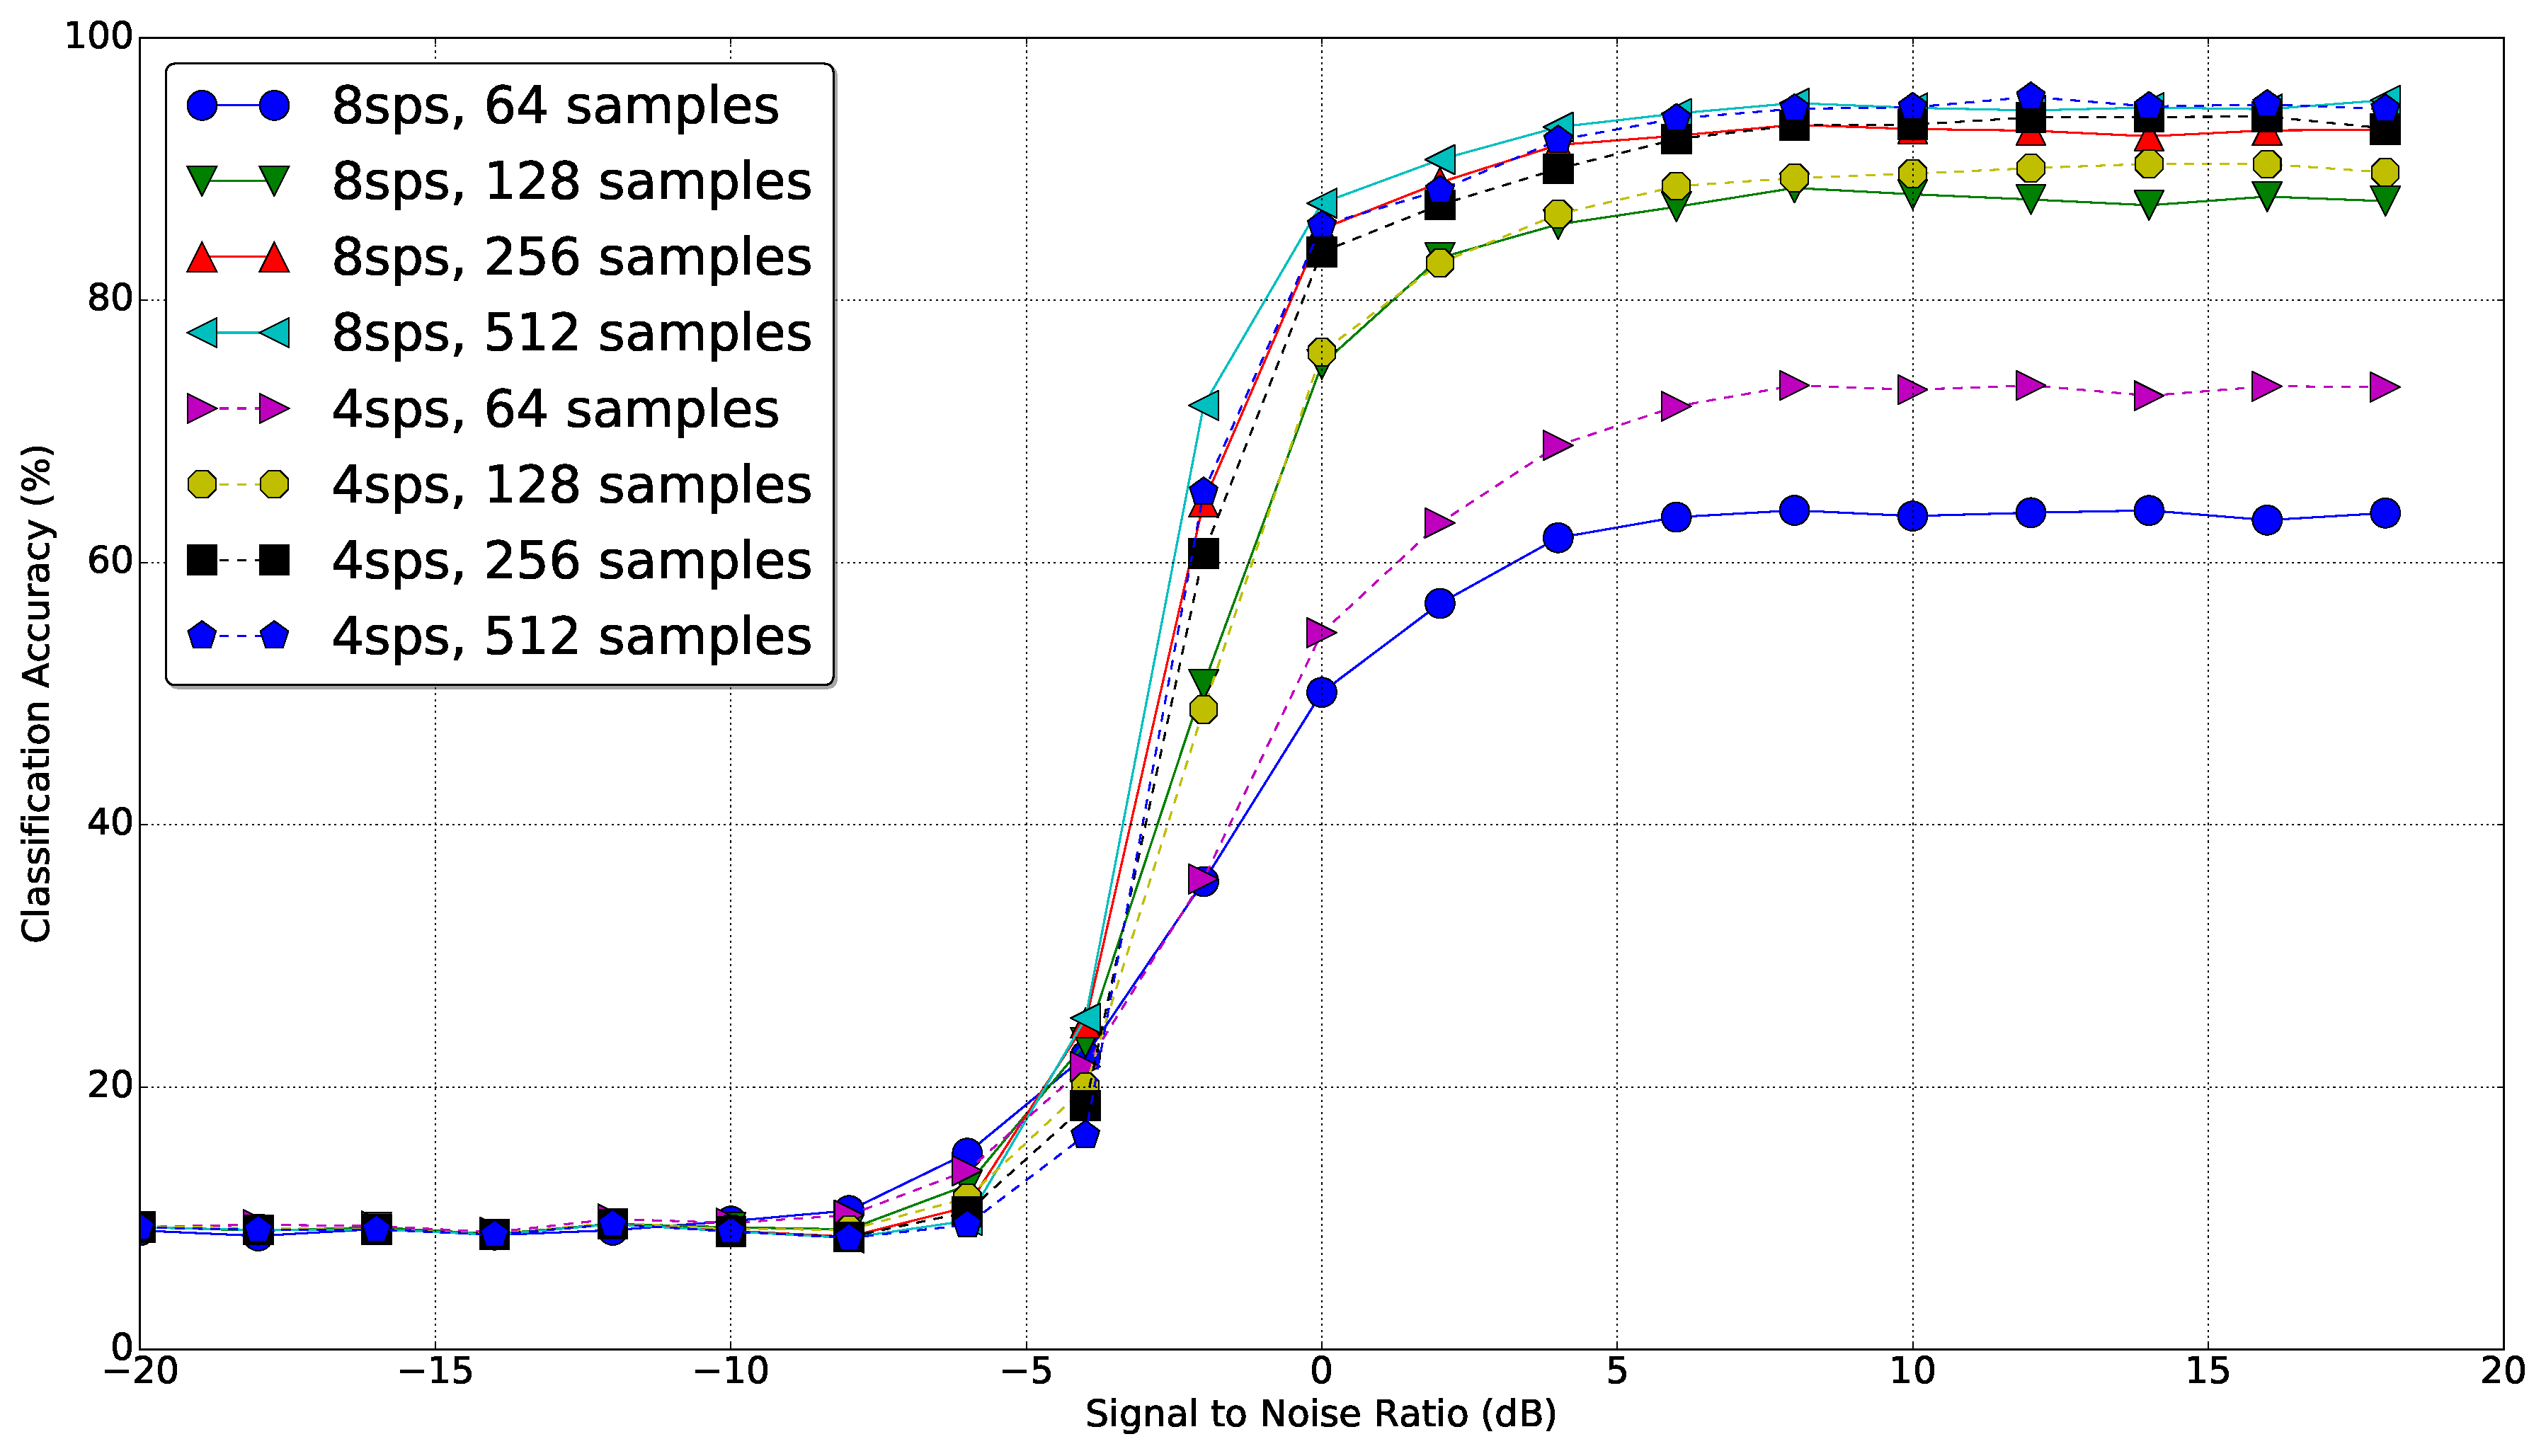
\includegraphics[width=\columnwidth]{sections/lstm_accuracy.pdf}
% \caption{Classification accuracy for a model trained only on high SNR signals.}
% \label{fig_high_snr}
% \end{figure}

% \begin{figure}[!t]
% \centering
% \squeezeup
% %\resizebox{\columnwidth}{!}{\input{lstm_accuracy_lowsnr.pgf}}
% 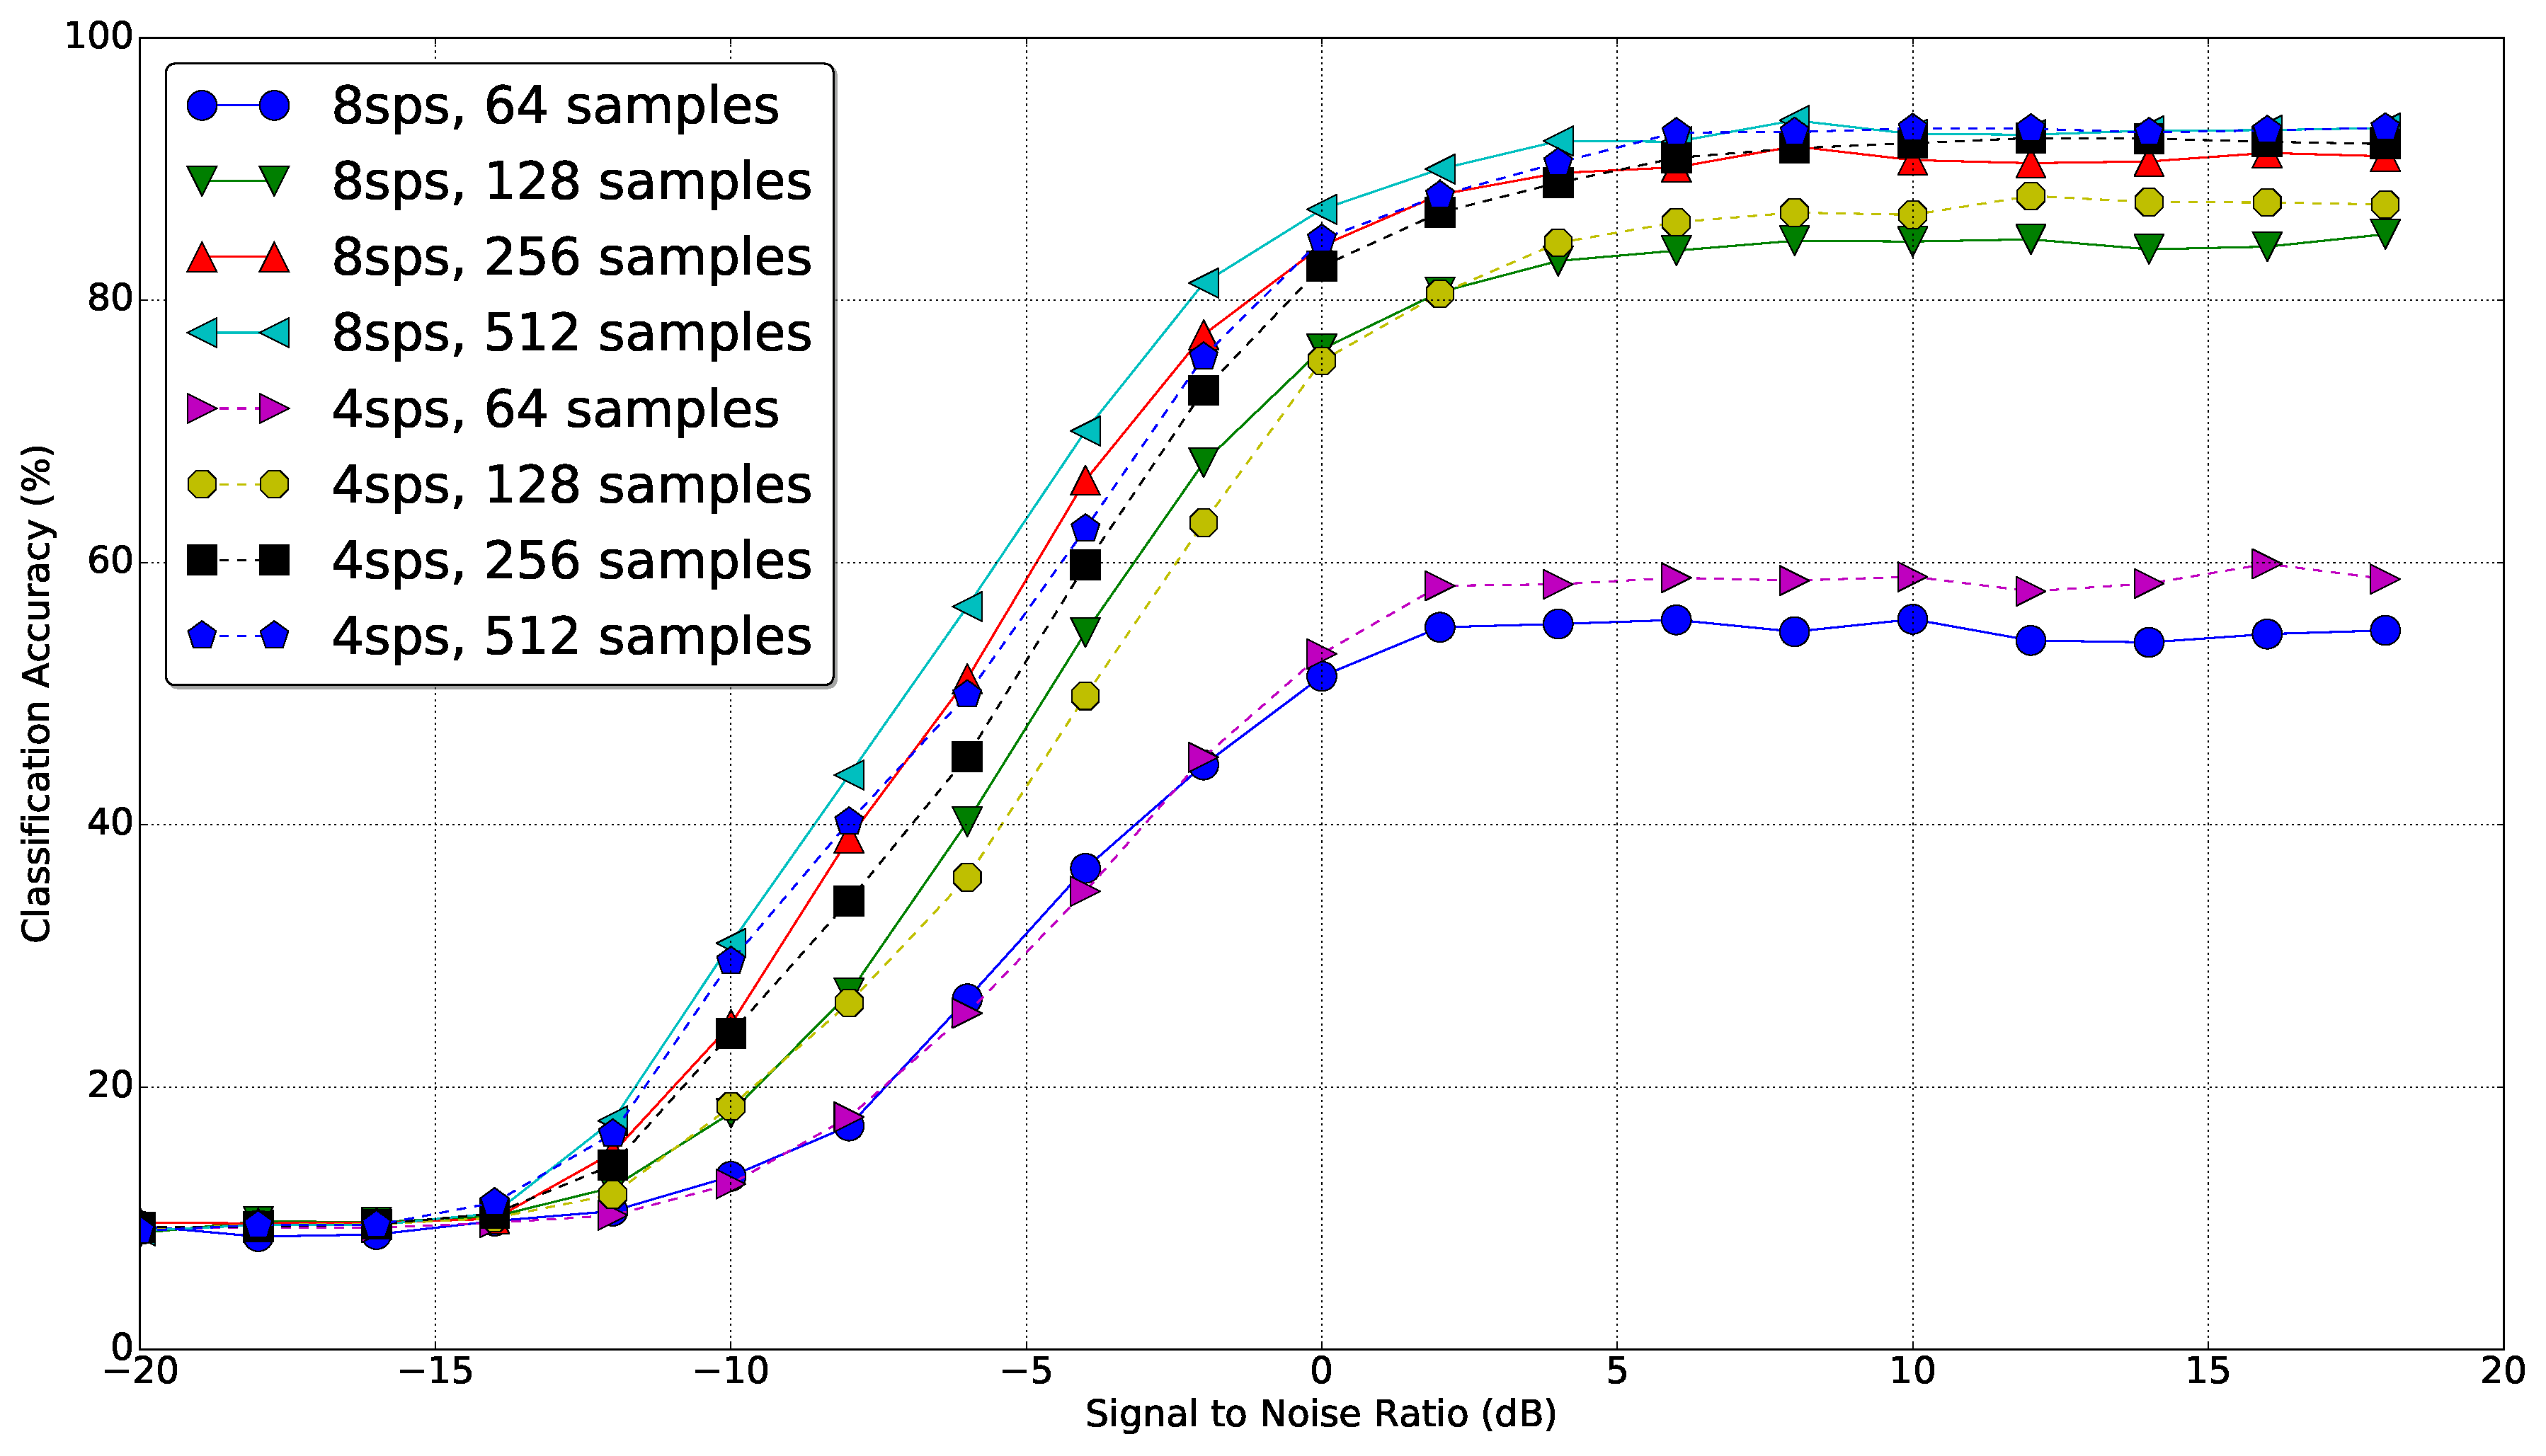
\includegraphics[width=\columnwidth]{sections/lstm_accuracy_lowsnr.pdf}
% \caption{Classification accuracy for a model trained on signals of all SNRs.}
% \label{fig_low_snr}
% \end{figure}



% \subsection{Performance comparison with CNN, and Cyclostationary models on RadioML dataset}
% \begin{itemize}
% \item Cyclostationary moments should be generated and we need to make sure that the selected moments/cumulants make sense. Please see Chad's analysis in his \href{https://cyclostationary.blog/2017/01/31/machine-learning-and-modulation-recognition-comments-on-convolutional-radio-modulation-recognition-networks-by-t-oshea-j-corgan-and-t-clancy/}{blog}.
% \item A little bit time consuming
% \end{itemize}

\subsection{Effect of cell size and layer depth}
\label{sec_hyperparams}


\begin{figure}[htb]
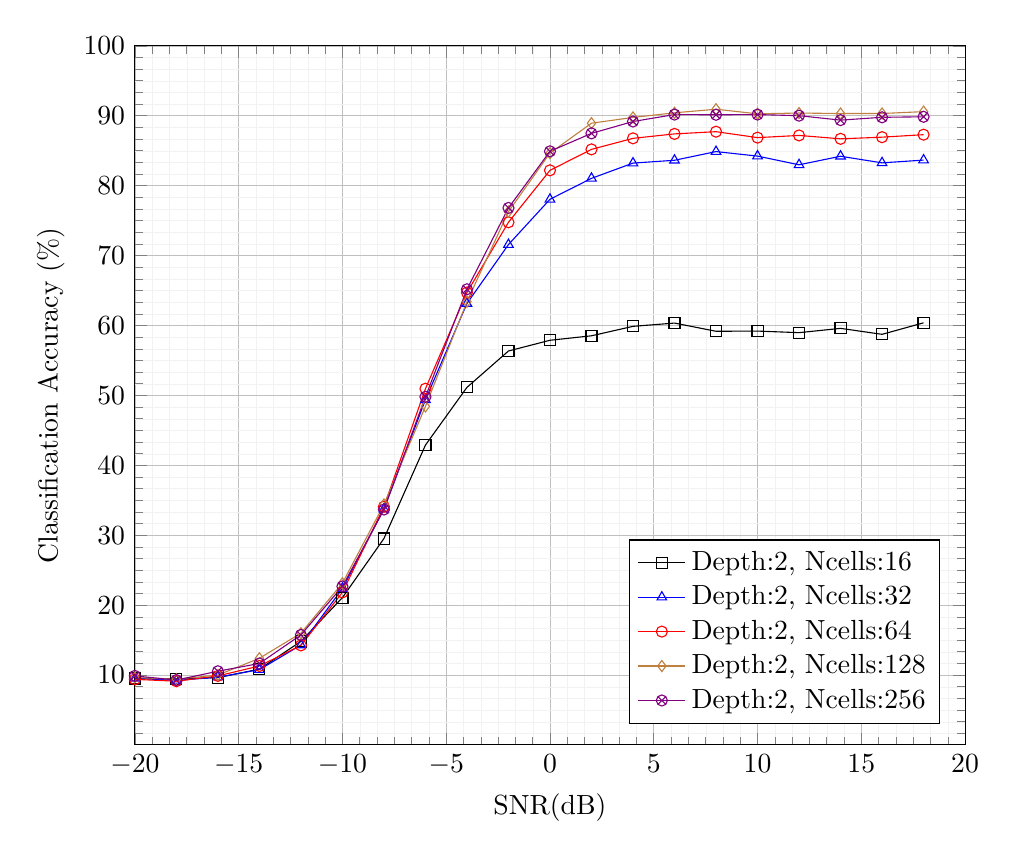
\begin{tikzpicture} \begin{axis}[legend pos=south east,
 width=\columnwidth,
 grid=both,
 ylabel=Classification Accuracy (\%),
  xlabel=SNR(dB),
 grid style={line width=.1pt, draw=gray!10},
 major grid style={line width=.2pt,draw=gray!50},
 minor tick num=5,
 xmin=-20,
 xmax=20,
 ymax=100,
 legend cell align={left},
]

\addplot[mark=square, color=black] coordinates { 
( -20 , 9.51509606587 )  ( -18 , 9.46412352407 )  ( -16 , 9.62373371925 )  ( -14 , 10.8444604836 )  ( -12 , 14.8040109389 )  ( -10 , 21.0769504176 )  ( -8 , 29.5241594709 )  ( -6 , 42.8885630499 )  ( -4 , 51.146025878 )  ( -2 , 56.3497822932 )  ( 0 , 57.8832116788 )  ( 2 , 58.524173028 )  ( 4 , 59.8751835536 )  ( 6 , 60.3429602888 )  ( 8 , 59.1704238052 )  ( 10 , 59.1985428051 )  ( 12 , 58.9715734202 )  ( 14 , 59.5866396014 )  ( 16 , 58.7330316742 )  ( 18 , 60.3780378038 ) 
};
\addlegendentry{Depth:2, Ncells:16}
\addplot[mark=triangle, color=blue] coordinates { 
( -20 , 9.53339432754 )  ( -18 , 9.22797456857 )  ( -16 , 9.69609261939 )  ( -14 , 10.7722843739 )  ( -12 , 14.2935278031 )  ( -10 , 22.3742669273 )  ( -8 , 33.731398126 )  ( -6 , 49.3768328446 )  ( -4 , 63.1423290203 )  ( -2 , 71.5711175617 )  ( 0 , 78.0474452555 )  ( 2 , 81.0432569975 )  ( 4 , 83.2232011747 )  ( 6 , 83.6281588448 )  ( 8 , 84.869251578 )  ( 10 , 84.2258652095 )  ( 12 , 82.9802643491 )  ( 14 , 84.203727625 )  ( 16 , 83.257918552 )  ( 18 , 83.6543654365 ) 
};
\addlegendentry{Depth:2, Ncells:32}
\addplot[mark=o, color=red] coordinates { 
( -20 , 9.38700823422 )  ( -18 , 9.11898274296 )  ( -16 , 9.87698986975 )  ( -14 , 11.2955611693 )  ( -12 , 14.2388331814 )  ( -10 , 21.8233516972 )  ( -8 , 34.0804703289 )  ( -6 , 50.9530791789 )  ( -4 , 64.7134935305 )  ( -2 , 74.7641509434 )  ( 0 , 82.1897810219 )  ( 2 , 85.1872046529 )  ( 4 , 86.7657856094 )  ( 6 , 87.4007220217 )  ( 8 , 87.7186654644 )  ( 10 , 86.8670309654 )  ( 12 , 87.1808799565 )  ( 14 , 86.6949621701 )  ( 16 , 86.9321266968 )  ( 18 , 87.2907290729 ) 
};
\addlegendentry{Depth:2, Ncells:64}
\addplot[mark=diamond, color=brown] coordinates {
( -20 , 9.64318389753 )  ( -18 , 9.40962761126 )  ( -16 , 10.003617945 )  ( -14 , 12.3962468423 )  ( -12 , 15.9890610757 )  ( -10 , 23.1384396659 )  ( -8 , 34.3927980893 )  ( -6 , 48.4237536657 )  ( -4 , 63.4011090573 )  ( -2 , 76.2880986938 )  ( 0 , 84.6532846715 )  ( 2 , 88.9312977099 )  ( 4 , 89.7577092511 )  ( 6 , 90.4151624549 )  ( 8 , 90.9287646528 )  ( 10 , 90.2732240437 )  ( 12 , 90.3856599674 )  ( 14 , 90.3118656579 )  ( 16 , 90.3167420814 )  ( 18 , 90.5850585059 ) 
};
\addlegendentry{Depth:2, Ncells:128}
\addplot[mark=otimes, color=violet] coordinates { 
( -20 , 9.88106129918 )  ( -18 , 9.28247048138 )  ( -16 , 10.5463096961 )  ( -14 , 11.6564417178 )  ( -12 , 15.7338195077 )  ( -10 , 22.6763817309 )  ( -8 , 33.6762814624 )  ( -6 , 49.7983870968 )  ( -4 , 65.1756007394 )  ( -2 , 76.8142235123 )  ( 0 , 84.9087591241 )  ( 2 , 87.4772809887 )  ( 4 , 89.1703377386 )  ( 6 , 90.1624548736 )  ( 8 , 90.1352569883 )  ( 10 , 90.1639344262 )  ( 12 , 90.0054318305 )  ( 14 , 89.3707326075 )  ( 16 , 89.7737556561 )  ( 18 , 89.8469846985 ) 
};
\addlegendentry{Depth:2, Ncells:256}
\end{axis}
\end{tikzpicture}
\caption{Classification accuracy of two layer amplitude-phase \ac{lstm} model for different cell sizes on RadioML dataset.}
\label{fig_depth_2}
\end{figure}



\begin{figure}[htb]
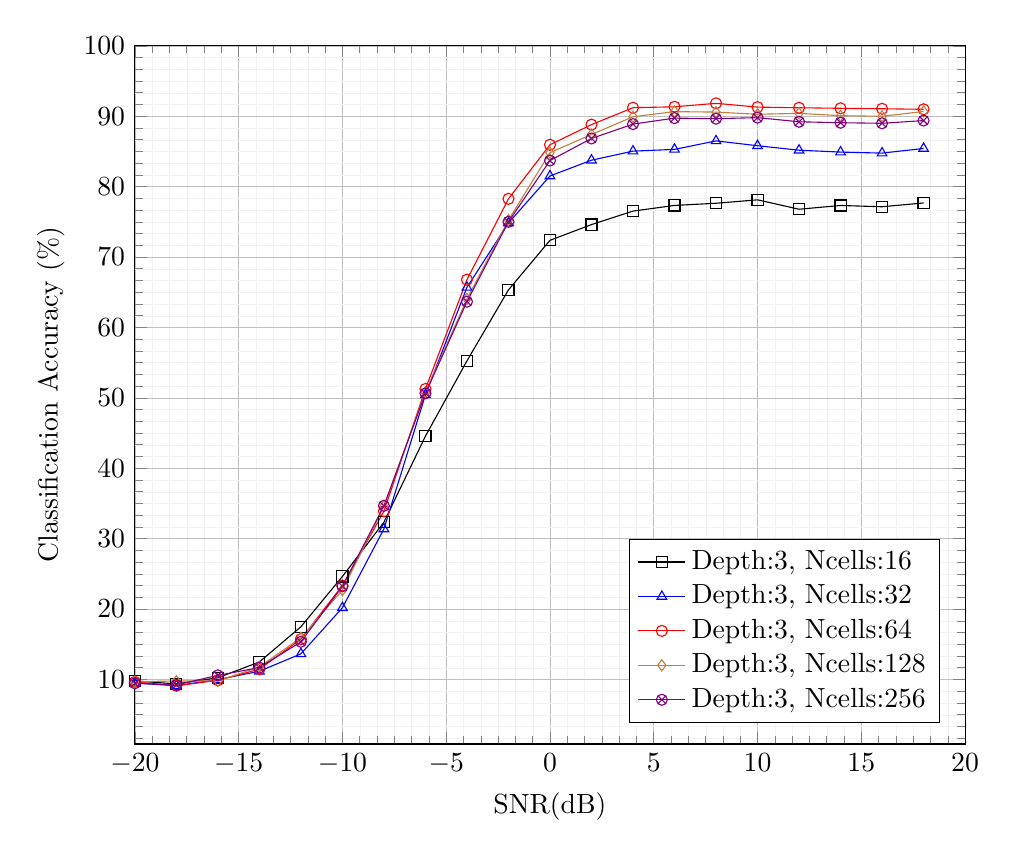
\begin{tikzpicture} \begin{axis}[legend pos=south east,
 width=\columnwidth,
 grid=both,
 ylabel=Classification Accuracy (\%),
  xlabel=SNR(dB),
 grid style={line width=.1pt, draw=gray!10},
 major grid style={line width=.2pt,draw=gray!50},
 minor tick num=5,
 xmin=-20,
 xmax=20,
 legend cell align={left},
]

\addplot[mark=square, color=black] coordinates { 
( -20 , 9.78956999085 )  ( -18 , 9.37329700272 )  ( -16 , 10.2387843705 )  ( -14 , 12.4864669794 )  ( -12 , 17.484047402 )  ( -10 , 24.631242225 )  ( -8 , 32.3351093147 )  ( -6 , 44.5564516129 )  ( -4 , 55.2495378928 )  ( -2 , 65.3301886792 )  ( 0 , 72.3722627737 )  ( 2 , 74.6092330062 )  ( 4 , 76.5234948605 )  ( 6 , 77.3285198556 )  ( 8 , 77.6375112714 )  ( 10 , 78.1238615665 )  ( 12 , 76.7879775484 )  ( 14 , 77.3205388448 )  ( 16 , 77.1402714932 )  ( 18 , 77.6777677768 ) 
};
\addlegendentry{Depth:3, Ncells:16}
\addplot[mark=triangle, color=blue] coordinates { 
( -20 , 9.47849954254 )  ( -18 , 9.11898274296 )  ( -16 , 9.98552821997 )  ( -14 , 11.1692529773 )  ( -12 , 13.6371923428 )  ( -10 , 20.1883774658 )  ( -8 , 31.3797538122 )  ( -6 , 50.4215542522 )  ( -4 , 65.6931608133 )  ( -2 , 74.8367198839 )  ( 0 , 81.5145985401 )  ( 2 , 83.7513631407 )  ( 4 , 85.0403817915 )  ( 6 , 85.2888086643 )  ( 8 , 86.4923354373 )  ( 10 , 85.810564663 )  ( 12 , 85.1711026616 )  ( 14 , 84.9049640155 )  ( 16 , 84.7601809955 )  ( 18 , 85.4185418542 ) 
};
\addlegendentry{Depth:3, Ncells:32}
\addplot[mark=o, color=red] coordinates { 
( -20 , 9.66148215919 )  ( -18 , 9.10081743869 )  ( -16 , 9.87698986975 )  ( -14 , 11.4579574161 )  ( -12 , 15.7338195077 )  ( -10 , 23.3339257153 )  ( -8 , 33.8967481168 )  ( -6 , 51.2646627566 )  ( -4 , 66.7837338262 )  ( -2 , 78.2656023222 )  ( 0 , 85.9489051095 )  ( 2 , 88.8040712468 )  ( 4 , 91.2077826725 )  ( 6 , 91.3357400722 )  ( 8 , 91.830477908 )  ( 10 , 91.2932604736 )  ( 12 , 91.2004345464 )  ( 14 , 91.1238235837 )  ( 16 , 91.0588235294 )  ( 18 , 90.9810981098 ) 
};
\addlegendentry{Depth:3, Ncells:64}
\addplot[mark=diamond, color=brown] coordinates { 
( -20 , 9.69807868253 )  ( -18 , 9.77293369664 )  ( -16 , 9.80463096961 )  ( -14 , 11.7827499098 )  ( -12 , 15.934366454 )  ( -10 , 22.69415319 )  ( -8 , 34.5948925225 )  ( -6 , 50.7881231672 )  ( -4 , 64.0480591497 )  ( -2 , 75.2539912917 )  ( 0 , 84.8175182482 )  ( 2 , 87.4045801527 )  ( 4 , 89.922907489 )  ( 6 , 90.6498194946 )  ( 8 , 90.5861136159 )  ( 10 , 90.2732240437 )  ( 12 , 90.4037660692 )  ( 14 , 90.071968998 )  ( 16 , 89.9909502262 )  ( 18 , 90.6750675068 )
};
\addlegendentry{Depth:3, Ncells:128}
\addplot[mark=otimes, color=violet] coordinates { 
( -20 , 9.46020128088 )  ( -18 , 9.22797456857 )  ( -16 , 10.5824891462 )  ( -14 , 11.6925297726 )  ( -12 , 15.3509571559 )  ( -10 , 23.2272969611 )  ( -8 , 34.6683814073 )  ( -6 , 50.6414956012 )  ( -4 , 63.6598890943 )  ( -2 , 75.0 )  ( 0 , 83.704379562 )  ( 2 , 86.8411486732 )  ( 4 , 88.8766519824 )  ( 6 , 89.7292418773 )  ( 8 , 89.6483318305 )  ( 10 , 89.7996357013 )  ( 12 , 89.2087633533 )  ( 14 , 89.0754751799 )  ( 16 , 88.9954751131 )  ( 18 , 89.3789378938 )
};
\addlegendentry{Depth:3, Ncells:256}
\end{axis}
\end{tikzpicture}
\caption{Classification accuracy of three layer amplitude-phase \ac{lstm} model for different cell sizes on RadioML dataset.}
\label{fig_depth_3}
\end{figure}

A comprehensive study is also performed to understand the effect of the number cells and layer depth on the model performance. The number of \ac{lstm} cells and layer depth are varied from 16 to 256 and  1 to 3 respectively. The models are trained on RadioML dataset on all \ac{snr}s. The accuracy levels for various layer depths are presented in Figures~\ref{fig_depth_1}, \ref{fig_depth_2} and \ref{fig_depth_3}. An initial analysis clearly shows that the model accuracy increases with increasing layer depth for mostly all cell sizes. It can be also noted that as the depth of the model increases, increasing the number of cells doesn't give much performance improvements. For instance, at depths 2 and 3 increasing the cell numbers from 128 to 256 doesn't provide any performance improvements.




% \subsection{Classification accuracy on real-life data}
% Add over the air results



\section{Conclusion and Future work}
\label{conclusion}
Wireless spectrum monitoring and signal classification over frequency, time and space dimensions is still an active research problem. In this paper we proposed a new \ac{lstm} based model which can classify signals with time domain amplitude and phase as input. \ac{soa} results on high \ac{snr}s (0 to 20dB) is achieved without using complex \ac{cnn}-\ac{lstm} models as mentioned in \cite{baseline}. Being a recurrent model we showed that the model can handle variable length inputs thus can capture sample rate variations effectively.



 %However, as there are various modulation schemes that exhibit same power spectral characteristics, which is well known in the research community, a detailed study is conducted on the complex \ac{iq} model variants. To also be able to handle such complex signals, a new \ac{lstm} based modulation classifier is proposed. 

%\sofie{I understand why you put magnitude FFT first: it is compliant with Electrosense. The full IQ study motivation is not that well introduced. Would it be useful to have also average phase FFT information? And compare then time versus frequency, phase verus amplitude, averaging versus full? Nowit is all a bit confusing...}

Though neural networks are good at function approximation, our experiments emphasize the fact that \emph{data preprocessing} and \emph{proper representation} are equally important. This claim is substantiated from our experiments with the \ac{lstm} model where the model gave poor results when fed with time domain \ac{iq} samples while it gave accuracies close to 90\% for high \ac{snr}s when provided with time domain amplitude and phase information. %\sofie{What about frequency domaing amplitude and phase?} 
 As shown by various \ac{soa} models in speech and image domains, performance improvements are seen with increasing layer depth which saturates after a few levels. In addition, we showed that basic technology classification is achievable by only using averaged magnitude \ac{fft} information over a distributed set of sensors complying with the uplink bandwidth resource constraints. Furthermore, experiments showed that quantized \ac{lstm} models can achieve good classification results thus reducing the processing power requirements at the cost of 10\% accuracy loss. This allows the deployment of these models on low cost sensors networks such as Electrosense enabling a wide area deployment. It is also remarkable that these deep learning models can classify signals with a fewer number of samples when compared to the expert feature variants, such as cyclic frequency estimators, enabling faster classification. Furthermore, deep learning allows for incremental learning, thus it would not be required to retrain the entire network from scratch for the new wireless non-idealities like antenna patterns and sensitivity. In addition, dedicated hardware is gaining popularity to reduce the deep learning model's energy and memory footprints which demands quantized versions of the models.

Although the \ac{lstm} models perform very well at high \ac{snr} conditions, CNN models seems to provide an additional 5-10\% accuracy on the low \ac{snr} conditions (SNRs below -2dB) as shown in \cite{baseline}. Even though we are not able to replicate the results in \cite{baseline} (%might be 
because of hyperparameter tuning), it is reasonable to conclude that the learned filters in CNN for a fixed sample rate might give performance improvements for low SNR values. Furthermore, all the implemented code for the proposed models are made publicly available for reproducing and verifying the results presented in this paper and for supporting future research.

Low \ac{snr} performance of these \ac{soa} deep learning models could be further improved with the help of efficient blind denoising models. Models which can perform automated channel equalization and compensate receiver imperfections such as frequency offset can further improve the classification performance. The current radio deep learning models make use of layers which basically applies non-linearity after simple multiply-accumulate-add operations while it is well established in the research community that cyclic cumulants, which are generated by time-shifted multiplication and averaging of the input itself, performs well in the expert feature space. Deep learning models which can extract features similar to cyclic cumulants might improve the performance metrics.

The analysis would not be complete without emphasizing the limitations of the \ac{soa} deep learning models. First, the current complex models are tested on a dataset with normalized bandwidth parameters. Real life transmitted signals generally have varying symbol rates and bandwidths. Even though the variable length \ac{lstm} model is shown to be capable of adapting to these scenarios, further analysis is required to validate the claim. %In addition, new datasets with more difficult modulation schemes like frequency-hopping and direct-sequence spread spectrum should be also tested. 
In future, models that can handle all possible spread spectrum modulations should be also tested. Second, the generalization capabilities of these models should be further investigated, in terms of performance of these models in unknown channel conditions and modulation parameters. Finally, most of the successful \ac{soa} models are supervised models which requires labeled training data. Labeling is a very tedious task which projects the importance of semi-supervised models for classification tasks. Published studies \cite{mlresource} on semi-supervised machine learning models for cellular network resource management validates the need for more semi-supervised models, which is also an active direction for future research. We believe deep learning models adapted to radio domain can help in understanding, analyzing and decision making in future complex radio environments.

% \section{Comments}
% \domenico{
\begin{itemize}
\item It is unclear why you need one layer for FFT magnitude and two layers for I/Q samples. What's the intuition? Can you use more layers also for FFT magnitude? Some discussion on the number of layers is done later, by it is not referenced while you introduce Fig1 and Fig2. 
\sreeraj{Added classification accuracy details for varying layer-depths and cell numbers for mag-FFT model too.}
\sofie{But this it is still confusing that you introduce a 1-layer for mag-FFT and 2-layer for IQ...}

\item A short intro to Sec III is also necessary. 
\sreeraj{Added a single line introduction.}
\item You present Fig. 3 and say that you cannot differentiate between LTE and DVB-T. As you said, this is expected, but I would also mention that this is expected because both are based on OFDM modulations. Right?
\sreeraj{Yes. Updated the argument in that section.}

\item In addition to that, it seems that you just give up and don't find a why to differentiate these technologies. One option is to switch and request IQ samples, the second could be to request smaller averaging time. But, in summary, I think you should propose a solution to differentiate the above technologies.
\sreeraj{Added switching to IQ pipeline as a solution. Averaging cannot help in the case of technologies with same PSD.}

\item Can you somehow unify Fig.1 and Fig.2 ? There are of components which are the same, and based on the input data, the number of layers is selected. It would give a more unified approach to the solution you propose.
\sreeraj{I can do that, but I it might complicate the input stream representation. Suggestions?}
\sofie{I agree you should combine. I also think you need a good notation for at or af, and relate it to the r(t) in the Eqs. 2 and 3. Can you come up with a generic model, where you enable both time and frequency domain representation (can you compare both) and averaging, and amplitude versus phase. For Mag-FFT, you throw away phase and also average, for compression reasons. }

\item The best would be of course to have a new section where all the components are put together in Electrosense, with the parameters such as number of layers and cell size that provide the right trade-off in performance in Electrosense network using ternary weights for IQ samples (when these are needed), and tested again. Most likely there will be new insights from the experimental evaluation (delays to make a decisions, reconfigure the nodes to switch to IQ samples, total amount of bandwidth requested before having a high confidence in your results, etc). This is probably quite some work.
\sreeraj{Indeed it is quite some work. We need to develop optimized implementations and the look into the processing and memory trade-offs. This is close to Vincent's second last comment. I will try to do an initial analysis at a theoretical level.}
\item In Conclusion section, I wouldn't say that frequency hopping and DSSS are more difficult. I would say that a methodology that can handle all possible spread spectrum modulations should be used.
\sreeraj{Done}
\end{itemize}
}

\vincent{
\begin{itemize}
\item You mention in the intro that spectrum monitoring is "extremely" challenging and that it is "multidisciplinary". You should give some arguments to back up these claims as it is not clear given the paper content.
\sreeraj{Done}
\item In the Intro, you say: we designed Electrosense. I would not write it like this as not all people that designed Electrosense are authors of this paper. You can rather say: "Electrosense was designed to address these challenges..."
\sreeraj{Done}
\item In Section II.A, you should better describe the Electrosense dataset. For example with information such as the sampling rate, dynamic range, averaging factors, sampling bandwidth, sweeping stratefy etc. Please also mention if the sensors were indoor/outdoor and that the captured signals were real signals captured over the air with an omnidirectional/discone? antenna.
\sreeraj{Done}
\item In section II.A: 60 seconds is not the time averaging but the time resolution. You should mention the averaging as well (I think 5 or 10 by default?). It is further not clear how you combine the averaged magnitude FFT from different bands as the sensor is constantly sweeping. I guess you combined different FFT scans since the technologies you analyze have a larger bandwidth than the sampling bandwidth of 2.4 MHz.
\sreeraj{Yes. Added more details on the dataset section to explain the combining too. Done.}
\item In Section II.B please explain how the RadioML2016 signals have been generated and captured (through a real radio frontend? If yes, please describe this acquisition setup.
\sreeraj{Added. Done.}
\item You never explicitly mention the classification problems you are trying to solve. I would introduce a new Section just before Section III to formalize the technology classification problem with averaged magnitude FFT data and the signal modulation classification problem with raw IQ data.
\sreeraj{Added a new section with problem formulation.}
\item Section III.A: It is not clear why you use only a single layer model for technology classification and higher layer models for complex signals:
\sreeraj{Included classification results for varying mag-FFT model layer depth and cell numbers. Added more details in the text.}
\item In Section III.B: You should mention here that you investigate 1, 2, and 3 layer models in this work (and not only 2 layers as stated here)
\sreeraj{Added. Done.}
\item In Section III.B: You should mention the option of using IQ samples instead of amplitude and phase as input and why IQ samples is expected to be worse. If you have the classification performance results with IQ samples, I would include them as well in the evaluation to show the impact of this design choice.
\sreeraj{Our standard 2 layer lstm model doesn't even converge during training when fed  with IQ data, giving a constant accuracy close to 9\% for 11 modulation schemes. Ran the models again on IQ data without any success. Updated this 9\% figure in the text. Not worth adding to the plots.}
\item In Figure 3: The dvb classification performance does not add to 1? Is this possible that the outcome is "not classified". All other classifications add up to 1!
\sreeraj{Nice catch. There was a bug in the confusion matrix plotting code for mag-FFT case. Fixed.}
\item In Section IV, first paragraph, you mention that in Electrosense the spectrum is averaged for a period of 60 seconds. This is not entirely true since the sensor is inspecting a specific band only every ~50 seconds. At time resolution of 60 seconds, the spectrum should be averaged over only two sensor scans and not the entire 60 seconds.
\sreeraj{True. Corrected it.}
\item In Section IV, second paragraph, Please explain in more details why the classification with magnitude FFT does not work for modulation classification.
\sreeraj{Added some more details. I can also add one figure showing same PSDs for multiple modulation schemes if it is required. Suggestions?}
\item I would put subsection IV.A in section III.
\sreeraj{Moved.}
\item Section IV.B, last sentence: Explain how you "normalize" amplitude and phase.
\sreeraj{Added normalization details.}
\item Figure 7: I would put here the performance of the 3-layer model since you have the results.
\sreeraj{Added.}
\item Section IV.F: I am missing here a result on computation efficiency. Can you provide results on CPU load of the different models? Currently, you do not really show that the quantized model is less resource intensive and that it works on a RPi platform.
\sreeraj{Evaluated binarized CNN model and gave some more insights how the performance improvements can be achieved on general/special purpose hardware. Proper resource reduction requires proper optimized implementation on RPi and benchmarking which can easily consume close to three weeks.}
\item The title is a little bit complex and not very self-explanatory. I will think of another candidate
\sreeraj{suggestions?}
\end{itemize}
}


% needed in second column of first page if using \IEEEpubid
%\IEEEpubidadjcol

% An example of a floating figure using the graphicx package.
% Note that \label must occur AFTER (or within) \caption.
% For figures, \caption should occur after the \includegraphics.
% Note that IEEEtran v1.7 and later has special internal code that
% is designed to preserve the operation of \label within \caption
% even when the captionsoff option is in effect. However, because
% of issues like this, it may be the safest practice to put all your
% \label just after \caption rather than within \caption{}.
%
% Reminder: the "draftcls" or "draftclsnofoot", not "draft", class
% option should be used if it is desired that the figures are to be
% displayed while in draft mode.
%
%\begin{figure}[!t]
%\centering
%\includegraphics[width=2.5in]{myfigure}
% where an .eps filename suffix will be assumed under latex, 
% and a .pdf suffix will be assumed for pdflatex; or what has been declared
% via \DeclareGraphicsExtensions.
%\caption{Simulation results for the network.}
%\label{fig_sim}
%\end{figure}

% Note that the IEEE typically puts floats only at the top, even when this
% results in a large percentage of a column being occupied by floats.


% An example of a double column floating figure using two subfigures.
% (The subfig.sty package must be loaded for this to work.)
% The subfigure \label commands are set within each subfloat command,
% and the \label for the overall figure must come after \caption.
% \hfil is used as a separator to get equal spacing.
% Watch out that the combined width of all the subfigures on a 
% line do not exceed the text width or a line break will occur.
%
%\begin{figure*}[!t]
%\centering
%\subfloat[Case I]{\includegraphics[width=2.5in]{box}%
%\label{fig_first_case}}
%\hfil
%\subfloat[Case II]{\includegraphics[width=2.5in]{box}%
%\label{fig_second_case}}
%\caption{Simulation results for the network.}
%\label{fig_sim}
%\end{figure*}
%
% Note that often IEEE papers with subfigures do not employ subfigure
% captions (using the optional argument to \subfloat[]), but instead will
% reference/describe all of them (a), (b), etc., within the main caption.
% Be aware that for subfig.sty to generate the (a), (b), etc., subfigure
% labels, the optional argument to \subfloat must be present. If a
% subcaption is not desired, just leave its contents blank,
% e.g., \subfloat[].


% An example of a floating table. Note that, for IEEE style tables, the
% \caption command should come BEFORE the table and, given that table
% captions serve much like titles, are usually capitalized except for words
% such as a, an, and, as, at, but, by, for, in, nor, of, on, or, the, to
% and up, which are usually not capitalized unless they are the first or
% last word of the caption. Table text will default to \footnotesize as
% the IEEE normally uses this smaller font for tables.
% The \label must come after \caption as always.
%
%\begin{table}[!t]
%% increase table row spacing, adjust to taste
%\renewcommand{\arraystretch}{1.3}
% if using array.sty, it might be a good idea to tweak the value of
% \extrarowheight as needed to properly center the text within the cells
%\caption{An Example of a Table}
%\label{table_example}
%\centering
%% Some packages, such as MDW tools, offer better commands for making tables
%% than the plain LaTeX2e tabular which is used here.
%\begin{tabular}{|c||c|}
%\hline
%One & Two\\
%\hline
%Three & Four\\
%\hline
%\end{tabular}
%\end{table}


% Note that the IEEE does not put floats in the very first column
% - or typically anywhere on the first page for that matter. Also,
% in-text middle ("here") positioning is typically not used, but it
% is allowed and encouraged for Computer Society conferences (but
% not Computer Society journals). Most IEEE journals/conferences use
% top floats exclusively. 
% Note that, LaTeX2e, unlike IEEE journals/conferences, places
% footnotes above bottom floats. This can be corrected via the
% \fnbelowfloat command of the stfloats package.


% if have a single appendix:
%\appendix[Proof of the Zonklar Equations]
% or
%\appendix  % for no appendix heading
% do not use \section anymore after \appendix, only \section*
% is possibly needed

% use appendices with more than one appendix
% then use \section to start each appendix
% you must declare a \section before using any
% \subsection or using \label (\appendices by itself
% starts a section numbered zero.)
%


\appendices
%\section{Proof of the First Zonklar Equation}
%Appendix one text goes here.

% you can choose not to have a title for an appendix
% if you want by leaving the argument blank
%\section{}
%Appendix two text goes here.


% use section* for acknowledgment
% \section*{Acknowledgment}


% The authors would like to thank...


% Can use something like this to put references on a page
% by themselves when using endfloat and the captionsoff option.
\ifCLASSOPTIONcaptionsoff
  \newpage
\fi



% trigger a \newpage just before the given reference
% number - used to balance the columns on the last page
% adjust value as needed - may need to be readjusted if
% the document is modified later
%\IEEEtriggeratref{8}
% The "triggered" command can be changed if desired:
%\IEEEtriggercmd{\enlargethispage{-5in}}

% references section

% can use a bibliography generated by BibTeX as a .bbl file
% BibTeX documentation can be easily obtained at:
% http://mirror.ctan.org/biblio/bibtex/contrib/doc/
% The IEEEtran BibTeX style support page is at:
% http://www.michaelshell.org/tex/ieeetran/bibtex/
%\bibliographystyle{IEEEtran}
% argument is your BibTeX string definitions and bibliography database(s)
%\bibliography{IEEEabrv,../bib/paper}
%
% <OR> manually copy in the resultant .bbl file
% set second argument of \begin to the number of references
% (used to reserve space for the reference number labels box)
%\balance
\bibliographystyle{IEEEtran}
\bibliography{sections/bibliography}

% \begin{IEEEbiography}[{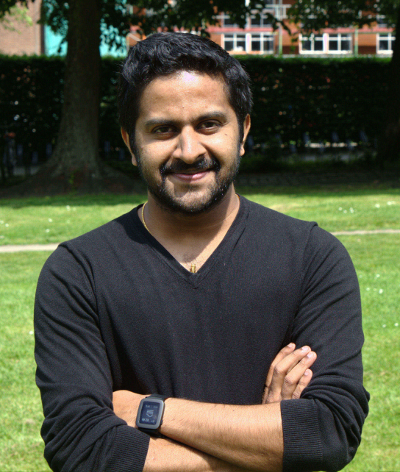
\includegraphics[width=1in,height=1.25in,clip,keepaspectratio]{figures/sreeraj}}]
    {Sreeraj Rajendran}
received his Masters degree in communication and signal processing from the Indian Institute of Technology, Bombay, in 2013. He is currently pursuing the PhD degree in the Department of Electrical Engineering, KU Leuven, Belgium. Before joining KU Leuven, he worked as a senior design engineer in the baseband team of Cadence and as an ASIC verification engineer in Wipro Technologies. His main research interests include machine learning algorithms for wireless and low power wireless sensor networks.
\end{IEEEbiography}


\begin{IEEEbiography}[{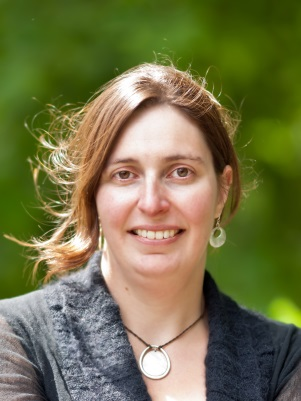
\includegraphics[width=1in,height=1.25in,clip,keepaspectratio]{figures/sofie}}]
    {Sofie Pollin}
obtained her PhD degree at KU Leuven with honors in 2006. From 2006-2008 she continued her research on wireless communication, energy-efficient networks, cross-layer design, coexistence and cognitive radio at UC Berkeley.  In November 2008 she returned to imec to become a principal scientist in the green radio team. Since 2012, she is tenure track assistant professor at the electrical engineering department at KU Leuven. Her research centers around Networked Systems that require networks that are ever more dense, heterogeneous, battery powered and spectrum constrained. Prof. Pollin is BAEF and Marie Curie fellow, and IEEE senior member. 
\end{IEEEbiography}
% biography section
% 
% If you have an EPS/PDF photo (graphicx package needed) extra braces are
% needed around the contents of the optional argument to biography to prevent
% the LaTeX parser from getting confused when it sees the complicated
% \includegraphics command within an optional argument. (You could create
% your own custom macro containing the \includegraphics command to make things
% simpler here.)
%\begin{IEEEbiography}[{\includegraphics[width=1in,height=1.25in,clip,keepaspectratio]{mshell}}]{Michael Shell}
% or if you just want to reserve a space for a photo:

% \begin{IEEEbiography}{Sreeraj Rajendran}
% Biography text here.
% \end{IEEEbiography}

% % if you will not have a photo at all:
% \begin{IEEEbiographynophoto}{Wannes Meert}
% Biography text here.
% \end{IEEEbiographynophoto}

% insert where needed to balance the two columns on the last page with
% biographies
%\newpage

% \begin{IEEEbiographynophoto}{Sofie Pollin}
% Biography text here.
% \end{IEEEbiographynophoto}

% You can push biographies down or up by placing
% a \vfill before or after them. The appropriate
% use of \vfill depends on what kind of text is
% on the last page and whether or not the columns
% are being equalized.

%\vfill

% Can be used to pull up biographies so that the bottom of the last one
% is flush with the other column.
%\enlargethispage{-5in}



% that's all folks
\end{document}


